%%%%%%%%%%%%%%%%%%%%%%%%%%%%%%%%%%%%%%%%%%%%%%%%%%%%%%%%%%%%%%%%%%%%%%%%%%%%%%
% ASU Dissertation Template
%%%%%%%%%%%%%%%%%%%%%%%%%%%%%%%%%%%%%%%%%%%%%%%%%%%%%%%%%%%%%%%%%%%%%%%%%%%%%%
% Copyright 2021 Robert W. Kutter (robert@kutterconsulting.com)
%
%   See also: http://kutterconsulting.com
%
% For guidance on using this file, see the README.
%
%%%%%%%%%%%%%%%%%%%%%%%%%%%%%%%%%%%%%%%%%%%%%%%%%%%%%%%%%%%%%%%%%%%%%%%%%%%%%%
% Preamble
%%%%%%%%%%%%%%%%%%%%%%%%%%%%%%%%%%%%%%%%%%%%%%%%%%%%%%%%%%%%%%%%%%%%%%%%%%%%%%
\newcommand*{\pointsize}{12pt}          %<Set the font size; make sure the size is correct
                                        %   for the font you will use
\documentclass[letterpaper,             % Use US letter-size paper
               oneside,                 % No verso and recto differences
               \pointsize]              % Uses the font size defined above
               {memoir}
\renewcommand{\cleardoublepage}%        % \cleardoublepage will create entirely blank
  {\clearpage}%                         %   pages depending on settings (e.g., usually
                                        %   before start of \mainmatter); redefine it here
                                        %   so that no entirely blank pages are created
                                        %   automatically
%%%%%%%%%%%%%%%%%%%%%%%%%%%%%%%%%%%%%%%
% (Some) Packages
%%%%%%%%%%%%%%%%%%%%%%%%%%%%%%%%%%%%%%%
\usepackage{graphicx}                   % For importing image files
\usepackage{etoolbox}                   % For advanced commands throughout preamble
\usepackage{microtype}                  %~Improves kerning and protrusion (optional);
                                        %   See here for an introduction:
                                        %   http://www.khirevich.com/latex/microtype/

\providetoggle{usemicrotype}            % TRUE = microtype is being used
\makeatletter                           %   (Used to turn of microtype protrusion in the
\@ifpackageloaded{microtype}%           %   table of contents.)
  {\settoggle{usemicrotype}{true}}%
  {\settoggle{usemicrotype}{false}}
\makeatother
\usepackage{changepage}                 % For changing page layout (e.g., margins) in the
                                        %   middle of the document
\usepackage{calc}					              % Calculate text widths; used in page layout
                                        %   changes
\usepackage{multirow,array}             % Adds multi row tables

%%%%%%%%%%%%%%%%%%%%%%%%%%%%%%%%%%%%%%%
% Title page, input
%%%%%%%%%%%%%%%%%%%%%%%%%%%%%%%%%%%%%%%
\listadd{\titlelines}%
  {Development, Implementation, and Impacts of}             %<Enter the title of the dissertation
\listadd{\titlelines}%
  {Novelty Detection Systems for Mission Operations}            % If you want to
                                        %   split the title across lines,
                                        %   use another \listadd command for the
                                        %   second line
\newcommand*\Author{Paul Alexander Horton}          %<Enter your name; must match official transcript
\newcommand*{\documentname}%
  {Dissertation}                        %<Enter the type of document (capitalized)
\newcommand*{\degreename}
  {Doctor of Philosophy}                %<Enter the type of degree (capitalized)
\newcommand*\defdate{June 2024}        %<Give month (written out fully) and year of
                                        %   the oral defense
\listadd{\committeechair}{Chris Groppi}   %<Enter committee chair name; use \listadd for
\listadd{\committeechair}{Jim Bell}%   for additional names
\newcommand*{\chairlabel}{Co-Chair}        %<If you have co-chairs, replace this text with
                                        %   'Co-Chair'
\listadd{\committeemember}{Hannah Kerner} %<Enter committee member names; use \listadd for
\listadd{\committeemember}{Philip Mauskopf} %   additional names
\listadd{\committeemember}{Nargess Memarsadeghi} %   additional names

\newcommand*{\gradmonth}{August}         %<Enter the graduation date; month can only be:
                                        %  May, August, or December
\newcommand*{\gradyear}{2024}           %<Enter the graduation year, e.g. 2014

\listadd{\keywords}{keyword 1}          %<Enter keywords; use \listadd for
\listadd{\keywords}{keyword 2}          %   additional names (up to 6)
\newcommand*{\graddate}{\gradmonth%     % Compose full graduation date
  \space\gradyear}

%%%%%%%%%%%%%%%%%%%%%%%%%%%%%%%%%%%%%%%
% Page layout
%%%%%%%%%%%%%%%%%%%%%%%%%%%%%%%%%%%%%%%
\settrimmedsize{\stockheight}%          % Specifies \paperheight and \paperwidth
  {\stockwidth}{*}
\settrims{0pt}{0pt}                     % Set location of page in relation to the stock.
                                        % Paper and stock size are equivalent,
                                        % so both \trimtop and \trimedge are set to 0pt
\newlength{\forfootskip}
\setlength{\forfootskip}%
  {3\baselineskip}
\newlength{\textblockheight}            % Calculate height of text block to leave room
\setlength{\textblockheight}{9.0in}     %   for footers, keeping page numbers outside
\addtolength{\textblockheight}%         %   the 1in vertical margins
  {-\forfootskip}
\settypeblocksize{\textblockheight}%    % Calculated by 1.0in vertical margins and
  {*}{*}                                %   letting margins set the width of the typeblock
\setulmargins{1.0in}{*}{*}              % Set upper margin (\uppermargin, not \topmargin);
                                        %   calculate the bottom margin
\setlrmarginsandblock{1.25in}{1.25in}{*}%~Set margins and calculate width of typeblock
\setheaderspaces{*}{0.5\baselineskip}{*}% Arguments: '\headdrop', '\headsep', and/or ratio
                                        %   Note: This is only used in the list of
                                        %   contents sections
\setheadfoot{\baselineskip}%            % Set '\headheight' and '\footskip'
  {\forfootskip}
\checkandfixthelayout                   % Required by memoir package after setting layout
\settypeoutlayoutunit{in}               % Write layout dimensions to log file in inches

%%%%%%%%%%%%%%%%%%%%%%%%%%%%%%%%%%%%%%%
% Fonts
%%%%%%%%%%%%%%%%%%%%%%%%%%%%%%%%%%%%%%%
\usepackage[T1]{fontenc}                % Standard option to handle, e.g., accented
                                        %   characters like 'ö' better
                                        
\usepackage{amssymb,mathtools}          % For AMS-LaTeX, see here for more:
                                        %     http://www.ams.org/publications/authors/tex/amslatex
                                        % ('mathtools' loads and extends 'amsmath')
\usepackage{ifxetex,ifluatex}           % Can check if XeTeX or LuaTeX was used to typeset
\usepackage{fixltx2e}                   % Provides \textsubscript
\IfFileExists{upquote.sty}%             % Use upquote if available, for
  {\usepackage{upquote}}{}              %   straight quotes in verbatim environments

% Load fonts depending on the
%   typesetting engine
\ifnum 0\ifxetex 1\fi\ifluatex 1\fi=0   % If pdftex
  \usepackage[utf8]{inputenc}           %   'utf8' should match the encoding of this file
                                        %
                                        %~Set up your font in pdftex here
                                        %
\else 									                % If xetex or luatex
  \ifxetex                              % If xetex
    \usepackage{mathspec}               % Matches non-math open-type font to math
                                        %   open-type font (use 'mathspec' if you want to
                                        %   write math in unicode)
    \usepackage{xunicode}               % Convert LaTeX character macros to unicode
  \else                                 % If luatex\usepackage{fontspec}
    \usepackage{fontspec}               % Use fontspec for (open type) font selection
  \fi
  \defaultfontfeatures{Mapping=tex-text,% Font spec setting
    Scale=MatchLowercase}
  \newcommand*{\euro}{€}

  % Using fonts in XeLaTeX can be complicated; the following settings
  % work when this file is compiled inside the Docker container produced
  % by the `build.sh` script.
  %
  % Sometimes something simple like the following will work:
  %
  % \setmainfont{Times12}
  %
  % But often the easiest solution is to move font files (*.otf or *.ttf) into
  % a sub-directory and provide the direct path to them here.
  %
  % See `fontspec` documentation for more on using local font files.
  %
  % \setmainfont{EBGaramond12}[           %<Set the main font; make sure the font is correct
  %                                       %   for the font size (See ASU Style Guide)
  %   Path          = /usr/share/fonts/opentype/ebgaramond/,
  %   Extension     = .otf ,
  %   UprightFont   = *-Regular ,
  %   ItalicFont    = *-Italic ,
  %   % Notice that bold is missing here because the Docker image does not have
  %   % a bold typeface for Garamond; it would probably be possible to find
  %   % one on your local system or online.
  % ]

%  \setmathfont(Digits,Latin,Greek)%     %~Uncomment two lines to set a font for math%
%    {MATHFONT}
\fi

%%%%%%%%%%%%%%%%%%%%%%%%%%%%%%%%%%%%%%%
% Line spacing
%%%%%%%%%%%%%%%%%%%%%%%%%%%%%%%%%%%%%%%
\DoubleSpacing                          % True double spacing
\BeforeBeginEnvironment{quote}          % Memoir leaves most special material
  {\par\SingleSpacing}                  %   single spaced, but makes block quotes
\AfterEndEnvironment{quote}%            %   double-spaced; fix to follow ASU style guide
  {\vspace{-\baselineskip} %
  \DoubleSpacing}
\BeforeBeginEnvironment{quotation}%
  {\par\SingleSpacing}
\AfterEndEnvironment{quotation}%
  {\vspace{-\baselineskip} %
  \DoubleSpacing}

\setlength{\footnotesep}{\baselineskip} % Double space *between* footnotes
\renewcommand*{\footnoterule}{%         % Redefine footnoterule so that initial footnote
  \kern-3pt%                            %   still appears right under the rule (changing
  \hrule width 0.4\columnwidth          %   \footnotesep also changes the space between the
  \kern 2.6pt                           %   rule and the first footnote
  \vspace{-0.5\baselineskip}            % (Here is the vertical space adjustment)
  }

\usepackage{enumitem}                   % Control spacing in enumerate environment
\setlist{noitemsep}                     % Remove extra vertical spacing between items in lists
                                        % \setlist{nosep} to leave no space around whole list

%%%%%%%%%%%%%%%%%%%%%%%%%%%%%%%%%%%%%%%
% Page numbering
%%%%%%%%%%%%%%%%%%%%%%%%%%%%%%%%%%%%%%%
\makepagestyle{ASU}
  \makeevenfoot{ASU}{}{\thepage}{}
  \makeoddfoot{ASU}{}{\thepage}{}

%%%%%%%%%%%%%%%%%%%%%%%%%%%%%%%%%%%%%%%
% Title page, formatting
%%%%%%%%%%%%%%%%%%%%%%%%%%%%%%%%%%%%%%%
\newlength{\savedfootskip}
\setlength{\savedfootskip}{\footskip}
\newcommand{\titlepagesetup}{%          % Page layout for title page
  \changepage%                          % Adjustment to page dimensions:
    {\savedfootskip}%                   %   text height
    {}%                                 %   text width
    {}%                                 %   even-side margin
    {}%                                 %   odd-side margin
    {}%                                 %   column sep.
    {}%                                 %   topmargin
    {}%                                 %   headheight
    {}%                                 %   headsep
    {-\savedfootskip}%                  %   footskip
}

\newcommand{\closetitlepagesetup}{%     % Undo set up for title page
  \changepage{-\savedfootskip}{}{}{}{}%
    {}{}{}{\savedfootskip}%
}

\makeatletter                           % Do not modify this section; Enter info above
\newcommand*{\titlepageASU}{
  \titlepagesetup
  \clearpage
  \begin{center}
  \SingleSpacing
  \thispagestyle{empty}
    \renewcommand*{\do}[1]{##1 \\[\baselineskip]}
    \dolistloop{\titlelines}
    by \\[\baselineskip]
    \Author \\[5\baselineskip]
    A \documentname~Presented in Partial Fulfillment \\
    of the Requirements for the Degree \\
    \degreename \\
    \vfill                              % Vertically center the portion below
    Approved \defdate~by the \\
    Graduate Supervisory Committee: \\[\baselineskip]
    \renewcommand*{\do}[1]{##1, \chairlabel \\}
    \dolistloop{\committeechair}
    \renewcommand*{\do}[1]{##1 \\}
    \dolistloop{\committeemember}
    \vfill                              % Vertically center the portion above
    ARIZONA STATE UNIVERSITY \\[\baselineskip]
    \graddate
  \end{center}
  \clearpage
  \closetitlepagesetup
}
\makeatother

%%%%%%%%%%%%%%%%%%%%%%%%%%%%%%%%%%%%%%%
% Heading styles
%%%%%%%%%%%%%%%%%%%%%%%%%%%%%%%%%%%%%%%
% Note: memoir also has \book and \part commands; do not use these
\makechapterstyle{ASU}{%                % Define chapter heading style
  \renewcommand*{\chapterheadstart}{}   % Chapter title flush with top margin
  \renewcommand*{\chapnamefont}%        % Set font for 'Chapter' or 'Appendix'
    {\normalfont}
  \renewcommand*{\chapnumfont}%         % Set font for number in chapter headings
    {\normalfont}
  \renewcommand*{\afterchapternum}%     % Insert a double line break after
    {\\[\baselineskip]}                 %   chapter number
  \renewcommand*{\chaptitlefont}%       % Set font for chapter title name
    {\normalfont}
  \setlength{\afterchapskip}{0pt}       % Set vertical space between chapter title and
                                        %   first paragraph; equivalent to one line break
                                        %   (vertical space = \afterchapskip + \baselineskip)
                                        % Note: This \afterchapskip value is only used in
                                        %   front matter
  \renewcommand*{\printchapternum}{%    % Center justify chapter number
    \centering \chapnumfont %
    \thechapter}
  \renewcommand*{\printchaptertitle}[1]%% Center justify
    {\expandafter\centering %           %   \MakeUppercase has issues; see here for some
    \expandafter\chaptitlefont %        %   details: https://tex.stackexchange.com/questions/35680/uppercase-in-newcommand
    \expandafter\MakeUppercase %        %   Accented characters and some fonts may not
    \expandafter{##1}}                  %   uppercase correctly; if that happens, just
                                        %   type the chapter title in uppercase
}

\setsecnumdepth{all}                    %~Enter the levels that you want to have numbered
                                        %   (Default is to number all [5 levels deep].)

\newcommand{\divisionbeforeskip}%       % Create default formatting for headings
  {\baselineskip}
\newcommand{\divisionindent}%
  {0.5em}
\newcommand{\divisionfont}{\normalfont} % Font must be \normalfont
\newcommand{\divisionafterskip}%
  {\baselineskip}

\setbeforesecskip{\divisionbeforeskip}  % Apply default formatting to all heading levels
\setsecindent{\divisionindent}          % Note: If you change \setsecnumdepth above, you
\setsecheadstyle{\divisionfont}         %   will need to set the indent for all lower
\setaftersecskip{\divisionafterskip}    %   levels to '0pt'; otherwise, they will be
                                        %   preceded by unnecessary space
\setbeforesubsecskip{\divisionbeforeskip}
\setsubsecindent{\divisionindent}
\setsubsecheadstyle{\divisionfont}
\setaftersubsecskip{\divisionafterskip}

\setbeforesubsubsecskip{\divisionbeforeskip}
\setsubsubsecindent{\divisionindent}
\setsubsubsecheadstyle{\divisionfont}
\setaftersubsubsecskip{\divisionafterskip}

\setbeforeparaskip{\divisionbeforeskip}
\setparaindent{\divisionindent}
\setparaheadstyle{\divisionfont}
\setafterparaskip{\divisionafterskip}

\setbeforesubparaskip{\divisionbeforeskip}
\setsubparaindent{\divisionindent}
\setsubparaheadstyle{\divisionfont}
\setaftersubparaskip{\divisionafterskip}

%%%%%%%%%%%%%%%%%%%%%%%%%%%%%%%%%%%%%%%
% Paragraph formatting
%%%%%%%%%%%%%%%%%%%%%%%%%%%%%%%%%%%%%%%
%\sloppybottom                          % Reduce the chances of widows
\raggedbottom                           % Loosens vertical spacing requirements, so
                                        %   \sloppybottom doesn't make pages look bad;
                                        %   it also prevents large gaps in the middle of
                                        %   pages and pushes them to the bottom of pages
\indentafterchapter                     % Overrides the default which is not to indent
                                        %   the first paragraph in a chapter, but it
                                        %   looks odd in some places to not indent
                                        %   paragraphs

%%% List Titles %%%
\renewcommand{\contentsname}%           % Set heading for each list
  {Table of Contents}%                  %   Formatted as chapter headings by default, so
\renewcommand{\listtablename}%          %   no additional heading formatting is needed
  {List of Tables}
\renewcommand{\listfigurename}%
  {List of Figures}

%%% Depth %%%
\settocdepth{subparagraph}              % Include 5 levels deep (all levels) in TOC

%%% Fonts %%%
\makeatletter%
\patchcmd{\l@part}%                     % Patch the command that writes part-level entries
    {\cftpartfont {#1}}%                %   to the table of contents, so they are in
    {\normalfont \texorpdfstring{%      %   'normalfont' and uppercase
      \uppercase{#1}}{{#1}} }%
    {\typeout{Success: Patch %
      'l@part' to uppercase %
      part-level headings in the %
      table of contents.}}%
    {\typeout{Fail: Patch %
      'l@part' to uppercase %
      part-level headings in the %
      table of contents.}}%
\makeatother%

\makeatletter%
\patchcmd{\l@chapapp}%                  % Patch the command that writes chapter-level
    {\cftchapterfont {#1}}%             %   entries to the table of contents, so they are
    {\normalfont \texorpdfstring{%      %   in 'normalfont' and uppercase
      \uppercase{#1}}{{#1}} }%
    {\typeout{Success: Patch %
      'l@chapapp' to uppercase %
      part-level headings in the %
      table of contents.}}%
    {\typeout{Fail: Patch %
      'l@chapapp' to uppercase %
      part-level headings in the %
      table of contents.}}%
\makeatother%

% If not using 'hyperref', use the following commands to adjust 'part' and 'chapter'
%   level headings in the TOC
%\renewcommand*{\cftpartfont}%          % Uppercase 'part' and 'chapter' headings
%  {\normalfont\MakeTextUppercase}      % Note: Sending \MakeTextUppercase to the TOC
%\renewcommand*{\cftchapterfont}%       %   conflicts with hyperref and breaks it!
%  {\normalfont\MakeTextUppercase}%

\usepackage{titlecaps}                  % Set up headline style for captions in the
                                        %   lists of tables and figures
                                        % Note: ASU style guide does not provide
                                        %   comprehensive guidelines for headlines, so
                                        %   Chicago style for headline style is used
                                        % Note: Last word in title is not explicitly
                                        %   capitalized; in general, these settings are
                                        %   broadly correct, but captions should be
                                        %   reviewed to ensure they are being capitalized
                                        %   properly
\Resetlcwords
\Addlcwords{a an the}                   % Leave articles lowercase
\Addlcwords{and but for or nor}         % Leave conjunctions lowercase
\Addlcwords{aboard about above across % % Leave all prepositions lowercase
  after against along amid among anti % %   (This is a [non-exhaustive] list of common
  around as at before behind below %    %   one-word prepositions)
  beneath beside besides between %
  beyond but by concerning considering %
  despite down during except excepting %
  excluding following for from in %
  inside into like minus near of off %
  on onto opposite outside over past %
  per plus regarding round save since %
  than through to toward towards under %
  underneath unlike until up upon %
  versus vs via with within without}
\Addlcwords{ according\space{to} %      % Leave two-word conjunctions lowercase
  ahead\space{of} apart\space{from} %   %   (This is a [non-exhaustive] list of common
  as\space{for} as\space{of} %          %   two-word prepositions.)
  as\space{per} as\space{regards} %
  aside\space{from} astern\space{of} %
  back\space{to} because\space{of} %
  close\space{to} due\space{to} %
  except\space{for} far\space{from} %
  in\space{to} inside\space{of} %
  instead\space{of} left\space{of} %
  near\space{to} next\space{to} %
  on\space{to} opposite\space{of} %
  opposite\space{to} out\space{from} %
  out\space{of} outside\space{of} %
  owing\space{to} prior\space{to} %
  pursuant\space{to} rather\space{than} %
  regardless\space{of} right\space{of} %
  subsequent\space{to} such\space{as} %
  thanks\space{to} that\space{of} %
  up\space{to}}

\renewcommand{\cfttableaftersnumb}%     % Put table captions in List of Tables in title
  {\titlecap}%                          %   case
\renewcommand{\cftfigureaftersnumb}%    % Put table captions in List of Figures in title
  {\titlecap}%                          %   case

\renewcommand*{\cftpartpagefont}%       % Use normal font for all page numbers
  {\normalfont}
\renewcommand*{\cftchapterpagefont}%
  {\normalfont}
\renewcommand*{\cftsectionpagefont}%
  {\normalfont}
\renewcommand*{\cftsubsectionpagefont}%
  {\normalfont}
\renewcommand*{\cftsubsubsectionpagefont}%
  {\normalfont}
\renewcommand*{\cftsubsubsectionpagefont}%
  {\normalfont}
\renewcommand*{\cftparagraphpagefont}%
  {\normalfont}
\renewcommand*{\cftsubparagraphpagefont}%
  {\normalfont}
\renewcommand*{\cftfigurepagefont}%
  {\normalfont}
\renewcommand*{\cfttablepagefont}%
  {\normalfont}

\cftpagenumbersoff{part}                % Turn off page numbers for 'part's, which are
                                        %   actually serving as headings within the TOC

%%% Vertical Space %%%
\setlength{\cftbeforepartskip}{0pt}     % Remove all additional vertical spacing so TOC
\setlength{\cftbeforechapterskip}{0pt}  %   is double spaced uniformly
\setlength{\cftbeforesectionskip}{0pt}
\setlength{\cftbeforesubsectionskip}{0pt}
\setlength{\cftbeforesubsubsectionskip}{0pt}
\setlength{\cftbeforeparagraphskip}{0pt}
\setlength{\cftbeforesubparagraphskip}{0pt}
\setlength{\cftbeforefigureskip}{0pt}
\setlength{\cftbeforetableskip}{0pt}

\renewcommand{\insertchapterspace}{%    % By default, extra vertical space (10pt) is
  \addtocontents{lof}%                  %   inserted between tables and figures from
    {\protect\addvspace{0pt}}%          %   different chapters; remove this extra space.
  \addtocontents{lot}%
    {\protect\addvspace{0pt}}%
}

%%% Horizontal Space %%%
\newlength{\levelindentincrement}       % Set indent to increase by the same amount for
\setlength{\levelindentincrement}{2em}  %   each level in the TOC; don't adjust figure
\newlength{\levelindent}                %   or table indents
\setlength{\levelindent}%
  {\levelindentincrement}
\setlength{\cftchapterindent}%
  {\levelindent}
\addtolength{\levelindent}%
  {\levelindentincrement}
\setlength{\cftsectionindent}%
  {\levelindent}
\addtolength{\levelindent}%
  {\levelindentincrement}
\setlength{\cftsubsectionindent}%
  {\levelindent}
\addtolength{\levelindent}%
  {\levelindentincrement}
\setlength{\cftsubsubsectionindent}%
  {\levelindent}
\addtolength{\levelindent}%
  {\levelindentincrement}
\setlength{\cftparagraphindent}%
  {\levelindent}
\addtolength{\levelindent}%
  {\levelindentincrement}
\setlength{\cftsubparagraphindent}%
  {\levelindent}
\addtolength{\levelindent}%
  {\levelindentincrement}

\setlength{\cftchapternumwidth}%        % Decrease space between number and heading for
  {0.85\cftchapternumwidth}             %   all heading levels
\setlength{\cftsectionnumwidth}%
  {0.85\cftsectionnumwidth}
\setlength{\cftsubsectionnumwidth}%
  {0.85\cftsubsectionnumwidth}
\setlength{\cftsubsubsectionnumwidth}%
  {0.85\cftsubsubsectionnumwidth}
\setlength{\cftparagraphnumwidth}%
  {0.85\cftparagraphnumwidth}
\setlength{\cftsubparagraphnumwidth}%
  {0.85\cftsubparagraphnumwidth}

% Calculate the indent to the first
% character in table and figure
% captions.
% This is more complicated because the
% document automatically considers
% the total number of figures and
% tables and increases the indent to
% make room for longer numbers.
\newcounter{totfigures}                 % Collect the total number of figures
\newcounter{tottables}                  % Collect the total number of tables

\providecommand\totfig{}                % Retrieve the total number of figures
\providecommand\tottab{}                % Retrieve the total number of tables

\makeatletter
\AtEndDocument{%                        % Store the totals
  \addtocounter{totfigures}{%
    \value{figure}%
  }%
  \addtocounter{tottables}{%
    \value{table}%
  }%
  \immediate\write\@mainaux{%
    \string\gdef\string\totfig{%
      \number\value{totfigures}%
    }%
    \string\gdef\string\tottab{%
      \number\value{tottables}%
    }%
  }%
}
\makeatother

% The calculation that appears inside
% this block needs to be done as the
% the document is written, not in the
% preamble. `\pretocmd` makes this
% calculation happen right before
% `\listoffigures` is executed.
\usepackage{calculator}
\pretocmd{\listoffigures}{%
  % Calculate the number of digits in
  % the total number of figures
  %
  % Here is the algorithm:
  %   Floor(Log10(\number)) + 1
  \MAX{\totfig}{1}{\figurecount}
  \LOG[10]{\figurecount}{\tempAfig}%
  \FLOOR{\tempAfig}{\tempBfig}%
  \ADD{\tempBfig}{1}{\digitsinfig}%     % Number of digits in number of figs
  %
  % Calculate space factor for figures
  % The space factor is just one less
  % than the number of digits, but it
  % must be at least 0.
  %
  \SUBTRACT{\digitsinfig}{1}{\tempDfig}%
  \MAX{\tempDfig}{0}{\tempEfig}%
  \MULTIPLY{\tempEfig}{0.55}{%
    \figspacefactor%                    % Space factor for figures in LOF
  }%
  % Apply the space factor for figures
  \setlength{\cftfigurenumwidth}{%      % Figure has the same 'level' as
    \cftchapternumwidth%                % 'chapter' in the figure list, so
  }%                                    % make the number spacing the same as
                                        % for chapters unless there are more
  \addtolength{\cftfigurenumwidth}{%    % than 9 figures; in that case, add
    \figspacefactor em%                 % extra space (as calculated in
  }%                                    % `\figspacefactor`
}{}{}

% Same space calculation for tables
\pretocmd{\listoftables}{%
  % Calculate the number of digits in
  % the total number of tables
  \MAX{\tottab}{1}{\tablecount}
  \LOG[10]{\tablecount}{\tempAtab}%
  \FLOOR{\tempAtab}{\tempBtab}%
  \ADD{\tempBtab}{1}{\digitsintab}%     % Number of digits in number of tabs
  % Calculate space factor for tables
  \SUBTRACT{\digitsintab}{1}{\tempDtab}%
  \MAX{\tempDtab}{0}{\tempEtab}%
  \MULTIPLY{\tempEtab}{0.55}{%
    \tabspacefactor%                    % Space factor for tables in LOT
  }%
  % Apply the space factor for tables
  \setlength{\cfttablenumwidth}{%
    \cftchapternumwidth%
  }%
  \addtolength{\cfttablenumwidth}{%
    \tabspacefactor em%
  }%
}{}{}

%%% Leaders/dots %%%
\renewcommand*{\cftdotsep}{1.7}         % Set distance between dots for all heading levels
\renewcommand*{\cftchapterleader}%      % Turn on dots for 'chapter' level
  {\normalfont\cftdotfill{\cftdotsep}}
\makeatletter                           % Bring leader dots over to page number (no gap)
  \renewcommand{\@pnumwidth}{1.55em}    %~Manually adjust
  \renewcommand{\@tocrmarg}{2.55em}
\makeatother

\renewcommand{\cfttableaftersnum}{.}    % Period after number in LOT
\renewcommand{\cftfigureaftersnum}{.}   % Period after number in LOF

%%% Printing List Titles and Headers in Content Lists
% Table of Contents (TOC)
\copypagestyle{ASUtoc}{ASU}%            % Page style for regular page in TOC
  \makeevenhead{ASUtoc}%
    {\leftmark}{}{Page}
  \makeoddhead{ASUtoc}%
    {\leftmark}{}{Page}

\copypagestyle{ASUtocFirst}{ASU}%       % Custom page headers for first page of TOC
  \makeevenhead{ASUtocFirst}%           %    (print out the title)
    {}%
    {\printchaptertitle{\contentsname}}%
    {}
  \makeoddhead{ASUtocFirst}%
    {}%
    {\printchaptertitle{\contentsname}}%
    {}

\renewcommand{\tocheadstart}{}%         % Usually content list titles are printed like
                                        %   chapter headings; empty that formatting

\renewcommand{\printtoctitle}[1]{}%     % Don't print TOC title using default method;
                                        %   it will be output in the header

\renewcommand{\aftertoctitle}{%         % On the first page of the TOC, print out the
  \thispagestyle{ASUtocFirst}%          %   TOC title using a custom page style and print
  \hfill Page\par%                      %   the heading for the page below in the regular
  }%                                    %   textbox
                                        % Note: Need '\par' before lists; see here: https://tex.stackexchange.com/questions/49882/yet-another-perhaps-a-missing-item-error

% List of Tables (LOT)
\copypagestyle{ASUlot}{ASU}%            % Page style for regular page in list of tables
  \makeevenhead{ASUlot}{Table}{}{Page}
  \makeoddhead{ASUlot}{Table}{}{Page}

\copypagestyle{ASUlotFirst}{ASU}%       % Custom page headers for first page of list of
  \makeevenhead{ASUlotFirst}%           %   tables (print out the title)
    {}%
    {\printchaptertitle{\listtablename}}%
    {}
  \makeoddhead{ASUlotFirst}%
    {}%
    {\printchaptertitle{\listtablename}}%
    {}

\renewcommand{\lotheadstart}{}%         % Usually content list titles are printed like
                                        %   chapter headings; empty that formatting;

\renewcommand{\printlottitle}[1]{}%     % Don't print LOT title using default method;
                                        %   it will be output in the header

\renewcommand{\afterlottitle}{%         % On the first page of the list of tables, print
  \thispagestyle{ASUlotFirst}%          %   out the title using a custom page style and
  Table\hfill Page\par}%                %   print heading below in regular textbox

% List of Figures (LOF)
\copypagestyle{ASUlof}{ASU}
  \makeevenhead{ASUlof}{Figure}{}{Page}
  \makeoddhead{ASUlof}{Figure}{}{Page}

\copypagestyle{ASUlofFirst}{ASU}%       % Custom page headers for first page of list of
  \makeevenhead{ASUlofFirst}%           %   figures (print out the title)
    {}%
    {\printchaptertitle{\listfigurename}}%
    {}
  \makeoddhead{ASUlofFirst}%
    {}%
    {\printchaptertitle{\listfigurename}}%
    {}

\renewcommand{\lofheadstart}{}%         % Usually content list titles are printed like
                                        %   chapter headings; empty that formatting

\renewcommand{\printloftitle}[1]{}%     % Don't print LOF title using default method;
                                        %   it will be output in the header

\renewcommand{\afterloftitle}{%         % On the first page of the list of figures, print
  \thispagestyle{ASUlofFirst}%          %   out the title using a custom page style and
  Figure\hfill Page\par}                %   print heading below in regular textbox

%%% Page layout (dimensions) for Contents Lists
\newlength{\verticalpush}               % Set up to change page dimensions for the table
                                        %   of contents
                                        % Push everything down so all the content is still
                                        %   1in from the top of the page, including the
                                        %   header, so the header is available for titles
                                        %   on the first page of contents lists and then
                                        %   the headings on subsequent pages
\setlength{\verticalpush}%              % Calculate difference between \headdrop and the
  {1.0in - \headdrop}                   %   total upper margin (1in), so you can push
                                        %   the top of the header down into the textbox

\newcommand{\contentslistsetup}{%       % Set up for contents lists
  \changepage%                          % Adjustment to page dimensions:
    {-\baselineskip}%                   %   text height
    {}%                                 %   text width
    {}%                                 %   even-side margin
    {}%                                 %   odd-side margin
    {}%                                 %   column sep.
    {\verticalpush}%                    %   topmargin
    {}%                                 %   headheight
    {}%                                 %   headsep
    {-\verticalpush+\baselineskip}%     %   footskip
}

\newcommand{\closecontentslistsetup}{%  % Undo set up for contents lists
  \changepage{\baselineskip}{}{}{}{}%
    {-\verticalpush}{}{}{\verticalpush-\baselineskip}%
}

% Content lists can also be output directly. If the following command were used, all the
%   headings would have to be output manually (i.e., can't rely on any memoir macros for
%   formatting or setting in contents lists headings and lists). It would be best to
%   create a custom macro, such as '\customtoc', to output headings and content lists
%   following the style guide.
%
% \makeatletter
%   \@starttoc{toc}
% \makeatother

% These pages partly explain why it's difficult to use 'afterpage' to change page layout
%   settings (essentially, it's because everything inside \afterpage has a local scope).
%   If it were possible to use 'afterpage' in that way, the content lists would  be
%   easier to format. A new page layout could be called after the first page of each
%   content  list. Instead, use page marks to get the layout required by the style guide.
% https://tex.stackexchange.com/questions/97126/attempts-to-manually-change-linewidth-ignored-by-latex
% https://tex.stackexchange.com/questions/85729/page-styles-only-work-for-thispagestyle-under-afterpage

%%%%%%%%%%%%%%%%%%%%%%%%%%%%%%%%%%%%%%%
% Footnotes and Endnotes
%%%%%%%%%%%%%%%%%%%%%%%%%%%%%%%%%%%%%%%
\usepackage{chngcntr}                   % Modify counters (e.g., for figures, footnotes)
\counterwithout*{footnote}{chapter}     % Make footnote numbering continuous throughout

\providetoggle{useendnotes}
\settoggle{useendnotes}{true}           %<Set to 'true' if you want to use endnotes
\iftoggle{useendnotes}{%                % Use the command \pagenote to create endnotes
                                        %   in the running text. They will be collected
                                        %   and printed in a 'Notes' section at the end
                                        %   of the document

  \makepagenote                         % Required in preamble if using endnotes
  \continuousnotenums                   % Numbering does *not* reset after each chapter
  \renewcommand*{\pagenotesubhead}[3]{} % No subheads inside note list (default is to
                                        %   divide them by chapter)
  \renewcommand*{\notenuminnotes}[1]%   % Remove extra space between note number and note
    {\normalfont #1.}                   %   text
  \renewcommand{\postnoteinnotes}%      % Double space *between* notes
    {\par\vspace{\baselineskip}}
}{}                                     % Do nothing here if not using endnotes

%%%%%%%%%%%%%%%%%%%%%%%%%%%%%%%%%%%%%%%
% Bibliography
%%%%%%%%%%%%%%%%%%%%%%%%%%%%%%%%%%%%%%%
\newcommand{\bibfilename}{%             %<Enter the name of the *.bib file containing the
  main.bib%                   %   reference information for sources cited in
}%                                      %   the text. God help you if you're doing
                                        %   citations manually.

\newcommand{\bibheading}{References}    %<Enter the heading for the references section:
                                        %   'References', 'Works Cited', or 'Bibliography'

\providetoggle{usebiblatex}             % True = a biblatex package is being used;
                                        %   False = 'natbib' is being used
\settoggle{usebiblatex}{false}           %~Set to 'false' to use 'natbib' intead of
                                        %   biblatex; I strongly recommend using biblatex
                                        %   because natbib is rather old and will break
                                        %   for innocuous things like underscores in URLs
\iftoggle{usebiblatex}{%                % Settings for citation package
%                                       % Settings for 'biblatex' or a version of
%                                       %   'biblatex'
  \usepackage[authordate,%
              backend=bibtex,%           % Recommend to use 'biber' instead of 'bibtex'
              doi=only,%                % Avoid printing URLs
              isbn=false]%              % Don't print ISBN numbers
              {biblatex-chicago}        %~Other possibilities include: 'biblatex',
                                        %   'biblatex-apa', and 'biblatex-mla'
  \bibliography{\bibfilename}
  \setlength{\bibitemsep}%              % Set vertical distance between
    {0.5\baselineskip}%                 %   bibliography entries
  \setcounter{biburlnumpenalty}{9000}   % Break URLs in bibliography across lines
  \setcounter{biburlucpenalty}{9000}
  \setcounter{biburllcpenalty}{9000}

  \usepackage[style=american,%          % Settings for quotation marks; load after
    english=american]{csquotes}%        %   'inputenc'; only use with biblatex; throws
  \MakeOuterQuote{"}%                   %   error when used with natbib
}{%                                     % Settings for 'natbib'
  \usepackage{natbib}%
  \newcommand{\natbibstyle}{%           %~Enter the name of the *.bst file to use to
    src/asudis%                         %   format citations with natbib. Default is
  }%                                    %   'asudis'. I do not know where 'asudis' came
                                        %   from, but apparently it formats citations
                                        %   correctly because it was included with the
                                        %   previous LaTeX template.
}

%%%%%%%%%%%%%%%%%%%%%%%%%%%%%%%%%%%%%%%
% Tables and figures
%%%%%%%%%%%%%%%%%%%%%%%%%%%%%%%%%%%%%%%
\captiondelim{. }                       %~Use period (.) after caption number instead of
                                        %   colon (:). Change according to style guide.
\captionstyle[\raggedright]%            % Set justifcation for [one line captions]
  {\raggedright}                        %   and {multiple line captions}
\setlength{\belowcaptionskip}{0pt}      % Bring caption down closer to figure/table
\makeatletter                           % Consecutive numbering throughout
  \counterwithout{figure}{chapter}      %   (including back matter)
  \counterwithout{table}{chapter}
  \renewcommand\@memfront@floats{}
  \renewcommand\@memmain@floats{}
  \renewcommand\@memback@floats{}
\makeatletter

\newcommand{\macrocapwrap}[1]{%         % Use this macro to place other macros inside
  {\bgroup\bgroup{{#1}}\egroup\egroup}% %   captions, e.g., '\macrocapwrap{\ref{figure1}}'
}%                                      % Note: Necessary due to the 'titlecaps' package
                                        %   which modifies contents of captions

%%% Tables %%%
%
% Note: 'memoir' natively supports commands from the following table-related packages:
%   tabularx, ccaption, booktabs.
% Everyone has particular ideas about how tables should look, so you may need to
%   load additional packages and modify the code below to get tables (and figures) to
%   look the way you want them to.
\setfloatadjustment{table}{\raggedright}% Left justify material inside table floats
\usepackage{tabu}                       % 'tabu' is an excellent table package; it can
                                        %   automatically size column widths and has a
                                        %   lot of customizations that other packages do
                                        %   not. It also has a 'longtabu' environment that
                                        %   emulates 'longtable' with additional features
                                        %   from the 'tabu' package. If you don't want
                                        %   to use it, you can comment this line out.
\BeforeBeginEnvironment{table}%         % Single space inside table environment
  {\SingleSpacing}
\AfterEndEnvironment{table}
  {\DoubleSpacing}

%%% Figures %%%
\setfloatadjustment{figure}%            % Left justify material inside figure floats
  {\raggedright}
\BeforeBeginEnvironment{figure}%        % Single space inside figure environment
  {\SingleSpacing}
\AfterEndEnvironment{figure}
  {\DoubleSpacing}

\makeatletter                           % Define custom macro called '\maxwidth{}' that
  \def\maxwidth#1{%                     %   allows you to specify the maximum width of an
    \ifdim%                             %   imported image. See below for an example.
      \Gin@nat@width>#1 #1%             %
    \else%                              % Source: http://tex.stackexchange.com/questions/86350/includegraphics-maximum-width
      \Gin@nat@width%
    \fi}
\makeatother
%
% Example \maxwidth:
%
%   \includegraphics[width=\maxwidth]{\textwidth}]{image.pdf}
%
% Note: This will keep an image inside the horizontal margins assuming the image starts
%   on the right margin (i.e., no horizontal space before the image).

%%%%%%%%%%%%%%%%%%%%%%%%%%%%%%%%%%%%%%%
% Hyperref settings
%%%%%%%%%%%%%%%%%%%%%%%%%%%%%%%%%%%%%%%

%%% URL Settings %%%
\PassOptionsToPackage{hyphens}{url}
\usepackage[breaklinks=true]{hyperref}  % 'hyperref' should be loaded at the end of the
                                        %   preamble; Note: the uppercasing commands used
                                        %   throughout the preamble can conflict with it,
                                        %   especially when non-standard fonts or
                                        %   different file encodings are used
\urlstyle{same}                         % Set URLs in the same font as regular text

\tolerance 1414                         % Help URLs from entering margins
\hbadness 1414                          %   Source: https://tex.stackexchange.com/questions/3033/forcing-linebreaks-in-url
\emergencystretch 1.5em
\hfuzz 0.3pt
\widowpenalty=10000
\vfuzz \hfuzz

%%% Create metadata strings
\usepackage{hyperxmp}                   % For metadata
\renewcommand*{\do}[1]{#1\ }%           % Build title string to output to pdf document
\newcommand*{\onelinetitle}{%
  \dolistloop{\titlelines}%
}
\edef\theonelinetitle%
  {\onelinetitle}

\renewcommand*{\do}[1]{{#1}\ }%          % Build keyword string to output to pdf document
\newcommand*{\pdfkeywordsstring}{%
  \dolistloop{\keywords}%
}
\edef\thepdfkeywordsstring%
  {\pdfkeywordsstring}

\newcommand*{\pdfcopyrightstring}%      % Build copyright message string
  {Copyright \copyright\space\gradyear\ by \Author.%
  {\space}All rights reserved.}

\ifpdf                                  % Build pdf creator string (for pdfTeX)
  \makeatletter
  \def\extractpdftexversion#1-#2-#3 #4%
    \@nil{#3}
  \edef\pdfcreator{pdfTeX \expandafter%
    \extractpdftexversion\pdftexbanner\@nil}
  \makeatother
\fi
\ifxetex                                % Build pdf creator string (for XeTeX)
  \edef\pdfcreator{XeTeX %
    \the\XeTeXversion\XeTeXrevision}
\fi

\edef\pdfsummary{%                      % Build pdf summary
  A \documentname Presented in\space
  Partial Fulfillment of the\space
  Requirements for a \degreename\space
  from Arizona State University}

%%% Enter metadata and other settings
\hypersetup{                            % Set pdf metadata
  pdftitle={\theonelinetitle},          % Title
  pdfauthor={\Author},                  % Author
  pdfcreator={\pdfcreator},             % Enter the TeX writer for good documentation
 %pdfproducer={},                       % Let 'pdfproducer' be filled automatically
  pdfsubject={\pdfsummary},             % Subject of the document
  pdfkeywords=\thepdfkeywordsstring,    % List of keywords
  hidelinks={true},                     % Links look like regular text (no colors, boxes)
  breaklinks={true},                    % Allow links to break across lines
}
\ifxetex                                % If processing with XeTeX
  \hypersetup{unicode=true}             % Must use 'true' in XeTeX
\else
  \hypersetup{unicode=true}             % Default is to use 'true' otherwise, as well
\fi
\ifpdf                                  % Copyright message; probably only works in pdfTeX
  \hypersetup{
    pdfcopyright={\pdfcopyrightstring},
    pdfinfo={%
      Copyright=\pdfcopyrightstring%
    }%
  }
\fi

\usepackage%
  [numbered,%                           % Include numbers of sections in bookmarks
  open%                                 % Bookmark tree already expanded when PDF opened
  ]%
  {bookmark}
\bookmark[page=1,rellevel=0,%           % Create bookmark of title page at root level
  keeplevel=true]{Title Page}
\preto{\tableofcontents}{%              % Create bookmark for TOC
  \hypertarget{tocpage}{}%
  \bookmark[dest=tocpage,rellevel=0,%
    keeplevel=true]{\contentsname}%
}

%%%%%%%%%%%%%%%%%%%%%%%%%%%%%%%%%%%%%%%
% Copyright page
%%%%%%%%%%%%%%%%%%%%%%%%%%%%%%%%%%%%%%%
\newcommand{\copyrightpageASU}{%        % Create copyright page
  \thispagestyle{empty}
  \titlepagesetup
  ~\\ \vfill
    \begin{center}
      \copyright\gradyear\space%
      \Author\\%
      All Rights Reserved%
    \end{center}%
  \clearpage%
  \closetitlepagesetup
}

%%%%%%%%%%%%%%%%%%%%%%%%%%%%%%%%%%%%%%%
% Biographical Sketch
%%%%%%%%%%%%%%%%%%%%%%%%%%%%%%%%%%%%%%%

% Wrapper for entering a biographical
% sketch. This command takes a single
% argument, which is the text of the
% biographical sketch. It is allowed
% to use `\input` with an external
% file containing the text of the
% biographical sketch.
\newcommand{\biographicalsketch}[1]{%
  \bookmarksetup{startatroot}%
  \chapter*{Biographical Sketch}%
  \phantomsection%                      % Need for hyperref
  \addcontentsline{toc}{chapter}{%      % Add a chapter-level heading for
    \hspace{-\cftchapterindent}%        %  a biographical sketch to the ToC
    Biographical Sketch%
  }%

  #1
}

%%%%%%%%%%%%%%%%%%%%%%%%%%%%%%%%%%%%%%%
% Sample settings
%%%%%%%%%%%%%%%%%%%%%%%%%%%%%%%%%%%%%%%
\providetoggle{sample}                  % True = demonstration of template
\settoggle{sample}{false}
\iftoggle{sample}{%
  \newcounter{tablecounter}
  \setcounter{tablecounter}{1}
  \newcounter{figurecounter}
  \setcounter{figurecounter}{1}
}{%
}

%%%%%%%%%%%%%%%%%%%%%%%%%%%%%%%%%%%%%%%
% Debugging Help
%%%%%%%%%%%%%%%%%%%%%%%%%%%%%%%%%%%%%%%
\usepackage{lipsum}                     % Outputs dummy text

%%%%%%%%%%%%%%%%%%%%%%%%%%%%%%%%%%%%%%%%%%%%%%%%%%%%%%%%%%%%%%%%%%%%%%%%%%%%%%
% Document
%%%%%%%%%%%%%%%%%%%%%%%%%%%%%%%%%%%%%%%%%%%%%%%%%%%%%%%%%%%%%%%%%%%%%%%%%%%%%%
\begin{document}

\pagenumbering{Alph}                   % Set page numbering to a page numbering
                                       %   style that is not used anywhere else
                                       %   in the document. This is necessary
                                       %   because the title and copyright
                                       %   pages received numbers (even though)
                                       %   they're hidden) and some automatic
                                       %   reference packages (like glossary)
                                       %   will make references to the title
                                       %   or copyright page when there are
                                       %   crossreferences on the first or
                                       %   second page of a section that uses
                                       %   the same numbering system as the
                                       %   title and copyright pages. For
                                       %   example, if page i contains a
                                       %   glossary entry, the glossary would
                                       %   contain an automatic reference that
                                       %   skips to the title page instead of
                                       %   page i.

%%%%%%%%%%%%%%%%%%%%%%%%%%%%%%%%%%%%%%%
% Title page
%%%%%%%%%%%%%%%%%%%%%%%%%%%%%%%%%%%%%%%
\titlepageASU

%%%%%%%%%%%%%%%%%%%%%%%%%%%%%%%%%%%%%%%
% Copyright page
%%%%%%%%%%%%%%%%%%%%%%%%%%%%%%%%%%%%%%%
\copyrightpageASU                       %~If you don't want to have a copyright page,
                                        %   comment out this line

%%%%%%%%%%%%%%%%%%%%%%%%%%%%%%%%%%%%%%%
% Front matter
%%%%%%%%%%%%%%%%%%%%%%%%%%%%%%%%%%%%%%%
\chapterstyle{ASU}
\pagestyle{ASU}
\frontmatter

\chapter*{Abstract}                     % Abstract is required
NASA missions are producing increasingly large and complex datasets, placing significant demands on mission operations teams to analyze, prioritize, and react to scientific data in near real-time.
This dissertation presents the development, implementation, and evaluation of novelty detection systems designed to support mission operations across multiple fields of space science, including planetary exploration and astrophysics.
Additionally, this work spans multiple domains, such as tactical planning, integration and testing, and onboard analysis, demonstrating the versatility of novelty detection techniques in various contexts.
Often in mission operations, typical data is well understood, but unexpected data is difficult to identify and react to in a timely manner.
Novelty detection algorithms identify anomalous or atypical features in data by measuring their deviation from a population, offering the potential to improve the efficiency and effectiveness of mission operations teams by triaging data for prioritization in analysis and decision-making.

This dissertation approaches implementation of novelty detection systems in three primary domains.
The first domain integrates novelty detection into tactical operations for the Mars Science Laboratory Curiosity rover, operationalizing previously developed algorithms to identify novel features in multispectral Mastcam images.
The second domain develops time-series anomaly detection methods for the Roman Space Telescope's Wide Field Instrument, using both statistical and data-driven approaches to locate cosmic ray events and snowballs in detector readout ramps.
The third domain applies novelty detection directly onboard the Astrophysics Stratospheric Telescope for High Spectral Resolution Observations at Submillimeter-wavelengths (ASTHROS) balloon observatory, enabling real-time identification of problematic spectra during flight operations.
ASTHROS represents a major part of this dissertation, as I oversaw the development of the software for the entire readout system, providing the framework for the onboard novelty detection system.
I also collaborated with the ASTHROS science team to analyze analogous data from the Stratospheric Observatory for Infrared Astronomy (SOFIA) to generate maps of [NII] emission spectra and electron density in Carina Nebula, a task ASTHROS will perform during its flight.
The results of this work culminate in a modular software suite for ASTHROS capable of performing real-time data analysis and anomaly detection, providing a powerful tool for future balloon-borne astrophysics missions.             %<Enter the name of the .tex file containing your
                                        %   your abstract or omit this line and type in
                                        %   your abstract here.

\chapter*{Dedication}                   %~Dedication is optional
%\clearpage                             %~If you don't wish to display the heading
                                        %   'Dedication', comment out the previous line
                                        %   and use this one instead.
\leavevmode\vfill
To my cat, who had to put up with me harassing her every time I needed a break.
\vfill           %<Enter the name of the .tex file containing your
                                        %   your dedication or omit this line and type in
                                        %   your dedication here.

\chapter*{Acknowledgments}              %~Acknowledgments are optional
First and foremost, I would like to thank my co-chairs, Chris Groppi and Jim Bell, for their invaluable guidance and support throughout my growth as a researcher.
Between the two of you, you have taught me to be a better engineer and scientist, and encouraged me to find as many ways to combine those two as possible.
You gave me the freedom to explore my interests and the guidance to keep me on track when I was too zoomed in to see the bigger picture.
I would especially like to thank Chris for not only being an amazing mentor, but also a great friend.
In addition, I would also like to thank my committee members, Hannah Kerner, Phil Mauskopf, and Nargess Memarsadeghi for their contributions and mentorship throughout the years. 

I would like to thank Jose Siles, Jon Kawamura, Jorge Pineda, and the rest of the ASTHROS team for their support and collaboration.
Without Jose's trust in me to take on the role of Software Lead as a graduate student, I would not have had the opportunity to work on such an amazing project.
We have spent countless hours working together to make ASTHROS a reality, and I could not have asked for a more fulfilling project to work on.
In the same vein, I would like to thank both the Roman Space Telescope Wide Field Instrument Science Data Pipeline (RST WFI SDP) team and the Machine Learning and Instrument Autonomy (MLIA) group for all of your support and collaborations.

I would also like to thank my fellow graduate students, especially those in the basement, for their years of friendship.
Without people like, Libby Berkhout, Amy Zhao, Ryan Stephenson, Cody Roberson, Justin Mathewson, Cassandra Whitton, Jonathan Greenfield, Emily Lunde, Mohini Jodhpurkar, Jenna Moore, Isaac Smith, Kyle Massingill, Madeline Hedges, Ricardo Rodriguez, Daniel Lu, Sean Bryan, Tom Mozden, Talia Saeid, Caleb Wheeler, Eric Weeks, Ryan Stephenson, Adrian Sinclair, Sam Gordon, Gena Pilyavsky, Marko Neric, Jacob Glasby, Farzad Faramarzi and many others, the ISTB4 would be a very dull place to work. 
For almost a decade, y'all have made the lab a second home for me and I am forever grateful for the stories, drinks, and laughs we have shared throughout our time together.
I would also like to thank Christian Thompson in particular for being a wonderful cook, an invaluable friend, a great roommate, and the very best mentee I could have ever asked for.

A special thanks go to the family and friends who have supported me throughout this journey. 
From very early on, my parents have always challenged me to be independent and to pursue my passions, both skills that have served me well throughout my time at ASU.
I would not be where I am today without their encouragement and support.
There are far too many friends to name individually, but I would like to thank you all for putting up with me being in school for so long and always being there whenever I needed a break from the lab.

I would also like to thank the NASA Jet Propulsion Laboratory (JPL) Strategic University Research Partnership, and the NASA Space Technology Graduate Research Opportunity for their financial support throughout my PhD. 
This work was supported by a NASA Space Technology Graduate Research Opportunity. 
It was an incredible privilege to have a fellowship that enabled me to never have to worry about funding for my frequent trips to JPL and conferences.

And finally, I would like to thank my partner, Cecilia La Place, for her never-ending love and lifelong collaboration. 
Pursuing a PhD is an endeavor in and of itself, but pursuing two PhDs at the same time is a whole other level of challenge.
Thank you for reminding me to take breaks and being a beacon of light whenever I was lost in the mind-numbing perpetuity of my own research.
Like research, life is not just about the results but the methods we develop along the way.
I am forever grateful for the methods we have developed to work together and eagerly look forward to our future work.      %<Enter the name of the .tex file containing your
                                        %   acknowledgments or omit this line and type in
                                        %   your acknowledgments here.

\iftoggle{usemicrotype}                 % If 'microtype' is in use, turn off protrusion
  {\microtypesetup{protrusion=false}}%  %   for TOC
  {}
\clearpage                              % Output table of contents on a new page
\contentslistsetup                      % Change page layout for contents lists

\pagestyle{ASUtoc}
\tableofcontents*                       % Starred version leaves TOC heading out of TOC
\addtocontents{toc}%                    % List of ... needs to be on left margin, but
  {\setlength{\cftchapterindent}%       %   they inherit 'chapter' formatting, so override
    {0em}%
  }

\clearpage
\ifnumcomp{\tottab}{>}{0}{%
  \pagestyle{ASUlot}
  \listoftables                         % List of Tables should appear in TOC, so use
                                        %   unstarred version of \listoftables
  \clearpage
}{}

\ifnumcomp{\totfig}{>}{0}{%
  \pagestyle{ASUlof}
  \listoffigures                        % List of Figures should appear in TOC, so use
                                        %   unstarred version of \listoffigures
}{}

%\chapter{Definitions}                  %~OTHER LISTS (optional)
%\input{definitions}                    %<Enter the name of the .tex file or omit this
                                        %   line and type in here.

%\chapter{Preface}                      %~PREFACE (optional, less than 10 pages)
%\input{preface}                        %<Enter the name of the .tex file or omit this
                                        %   line and type in here.

\phantomsection                         % \phantomsection is needed before using
                                        %   \addtocontents when it contains certain macros
                                        %   when also using 'hyperref' package
\addtocontents{toc}%          -          % Undo manual override above for chapter indent,
  {\setlength{\cftchapterindent}%       %   so actual chapters in the TOC are indented
    {\levelindentincrement}%            %   correctly
  }
\setlength{\afterchapskip}%             % Set vertical space between chapter title and
  {\baselineskip}                       %   first paragraph; equivalent to two line breaks

\phantomsection
\addcontentsline{toc}{part}{Chapter}    % Add "Chapter" to TOC here at 'part' level
\phantomsection
\addtocontents{toc}%                    % Add this 'mark' to TOC so subsequent pages use
  {\protect\markboth{CHAPTER}{Page}}    %   the "CHAPTER" heading

\iftoggle{usemicrotype}                 % If 'microtype' is in use, turn protrusion back
  {\microtypesetup{protrusion=true}}%   %   on
  {}

\clearpage                              % Note: All these changes have to be above a
                                        %   a '\clearpage' before '\mainmatter'

\pagestyle{ASU}                         % Switch back to regular page style for remainder
                                        %   of the document
\closecontentslistsetup                 % Undo page layout for contents lists

%%%%%%%%%%%%%%%%%%%%%%%%%%%%%%%%%%%%%%%
% Body
%%%%%%%%%%%%%%%%%%%%%%%%%%%%%%%%%%%%%%%
\mainmatter
\chapter[Data Discovery Systems for Planetary Science]{Data Discovery Systems for Planetary Science}
\section{Abstract}
While innovations in scientific instrumentation have pushed the boundaries of Mars rover mission capabilities, the increase in data complexity has pressured Mars Science Laboratory (MSL) and future Mars rover operations staff to quickly analyze complex data sets to meet progressively shorter tactical and strategic planning timelines. 
MSLWEB is an internal data tracking tool used by operations staff to perform first pass analysis on MSL image sequences, a series of products taken by the Mast camera, Mastcam. Mastcam consists of a pair of 400-1000 nm wavelength cameras on MSL's Remote Sensing Mast that, among other functions, uses a filter wheel to produce multispectral images by creating a sequence of products at different wavelengths. 
Mastcam's multiband multispectral image sequences require more complex analysis compared to standard 3-band RGB images. 
Typically, these are analyzed by the inspection of false color images created to aid visualization, such as band ratios between different spectral indices that can highlight specific potential mineralogic differences among iron-bearing phases, and decorrelation stretches to enhance the color differences between multiple filters. 

Given the short time frame of tactical planning in which downlinked images might need to be analyzed (within 5-10 hours before the next uplink), there exists a need to triage analysis time to focus on the most important sequences and parts of a sequence. 
We address this need by creating products for MSLWEB that use novelty detection to help operations staff identify unusual data that might be diagnostic of new or atypical compositions or mineralogies detected within an imaging scene. 
This was achieved in two ways: 1) by creating products for each sequence to identify novel regions in the image, and 2) by assigning multispectral sequences a sortable novelty score. 
These new products provide colorized heat maps of inferred novelty that operations staff can use to rapidly review downlinked data and focus their efforts on analyzing potentially new kinds of diagnostic multispectral signatures. 
This approach has the potential to guide scientists to new discoveries by quickly drawing their attention to often subtle variations not detectable with simple color composites.
The products developed in this work have shown promising benefits for integration into mission operations by potentially decreasing tactical operations planning time through guided triage.
\section{Introduction}
While discovering the unexpected is one of the most exciting parts of research, the process of making a discovery often involves countless hours of sifting through otherwise mundane data. 
Advances in novelty detection systems can help to alleviate this arduous task by enabling researchers to focus their attention on the most interesting parts of their data. 
Novelty is defined as an unexpected occurrence in a sequence based on a data set of typical sequences.
Given what is known to be “normal,” the novelty detection algorithm highlights the most unusual features in an image. 
Novelty detection techniques work by analyzing the commonalities in a data set in order to generalize the structure of the data and pick out anomalies \cite{japkowicz1995novelty}.
When a new observation is presented to a novelty detection system, the system identifies features that differ from the commonalities learned during training \cite{markou2003novelty}.
This is different from traditional classification systems as what constitutes as \textit{novel} is not predefined. 
Instead of classifying samples as \textit{typical} and \textit{novel}, novelty detection systems build a model from \textit{typical} examples that can be used to discover anomalies. 
This makes novelty detection ideal for scenarios where \textit{novel} examples are infrequent or difficult to obtain and \textit{typical} examples are abundant \cite{japkowicz1995novelty}.
Identifying anomalous examples is useful in many application domains such as structural fault detection for aerospace systems by analyzing ambient vibrations \cite{worden1997structural} or identifying brain tumors using MRI images \cite{wang2020brain}.
\begin{figure*}
\centering
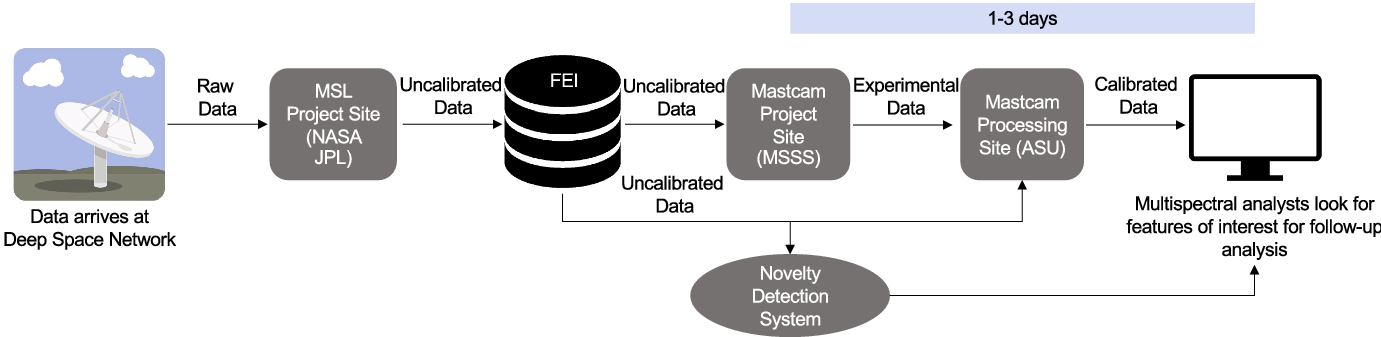
\includegraphics[width=\linewidth]{figs/1/DSN.png}
\caption[Mastcam Image Processing Pipeline]{\textbf{Illustration of the Mastcam image processing pipeline \protect\cite{kerner2020comparison}}}
\label{chap1/fig:timeline}
\end{figure*}

Planetary science is another domain where novelty detection proves useful. 
Due to the rapid turn-around required for tactical planning for landed Mars missions, efficient data analysis methods need to be employed to analyze data from scientific instruments \cite{bell2019tactical}.
With high volumes of downlinked data, tactical operations planning teams have to quickly perform ground analysis to meet the ten hour turn-around time for MSL operations to uplink commands \cite{samuels2013preparation}. 
The timeline is even shorter for the upcoming Mars 2020 mission which has a desired five hour turn-around time \cite{wilson2017nasa}.
During tactical planning, the MSL Curiosity rover sends compressed observations through one of three Mars orbiters to the Deep Space Network (DSN) on Earth so that operations team members can use these observations to make plans for the next sol \cite{kerner_multispec}.
Rapid analysis is required for tactical planning as discoveries made outside of the time frame are subject to increased mission resource cost as the rover may need to reverse course to re-visit the target \cite{kerner2020comparison}.
This need for rapid analysis makes systems that can quickly extract information and identify regions of interest in scientific data vital to efficient tactical planning. 

This work primarily focuses on the Mastcam imaging system on the MSL Curiosity rover.
Mastcam consists of a pair of multispectral Charge Coupled Device (CCD) imagers on MSL that are each capable of using an eight-position filter wheel to take red, green, and blue (RGB) images as well as multispectral images in nine bands from 400 to 1100 nm (visible to near-infrared) \cite{bell_mastcam}.
A set of image products from Mastcam is called a sequence.
Seven of the eight landed missions on Mars have employed camera systems capable of multispectral imaging \cite{bell2019tactical}.
Future missions, such as Mars 2020 and Psyche, will also be carrying similar multispectral cameras \cite{bell2016mastcam} \cite{bell_psyche}.
Given that multispectral cameras are so prevalent in planetary exploration, the ability to rapidly detect novel features in multispectral images is beneficial across many missions.

The goal of this work is to operationalize previous work developed for novelty detection for Mastcam.
\cite{kerner2020comparison} quantitatively compared different novelty detection methods for analysis of multispectral images on Mars.
With a typical data set, machine learning models including Reed-Xiaoli (RX) detectors, Principal Component Analysis (PCA), Generative Adversarial Networks (GANs), and Convolutional Autoencoders (CAE) were used to produce a measure of how atypical each image or multispectral pixel is in a new sequence. 
Using pixelwise analysis allows these methods to highlight difficult to identify novel regions within an image that may otherwise go undetected by operations staff.
These methods\footnote{https://github.com/JPLMLIA/mastcam-noveltydet} and the data set\footnote{https://zenodo.org/record/3732485} used to evaluate them were made publicly available at publication. 
Multiple models were evaluated to show that certain models perform better for certain novelties than others -- e.g., PCA was better suited for detecting spectral (compositional) novelties than for morphological (shape) novelties. 
Their work provides an in-depth qualitative evaluation between these methods which was used to guide decisions about which methods to use. 
While their work demonstrated the capabilities of the algorithms, it did not evaluate the methods based on their effectiveness in the tactical planning pipeline.
In order to be most useful to operations, these methods need to be automatically run on new data and integrated into tactical analysis workflows to accelerate tactical planning \cite{donahoe2020new}.
New advances in this work include further development of the algorithms and the creation of an implementation strategy for operations. 
Additionally, we analyzed the outputs from the system to determine the usefulness of these methods in comparison to existing tactical planning procedures. 

\section{Related Work}
Novelty detection is a form of anomaly detection that focuses on detecting novel examples in a data set \cite{domingues2019comparative}. 
Given what is known to be typical in a data set, these algorithms find novel examples that may be unknown to the user.
Unlike a classifier, novelty detection systems detect whether an input is similar to examples in the typical training set or if the input is novel \cite{markou2003novelty}.
Novelty detection can be seen as a one-class classification task where a model is trained to describe a data set of typical examples \cite{pimentel2014review}. 
For novelty detection, the training data represent a set of examples that an end user would identify as typical examples. 
When the model is used to infer the novelty of new data, the system calculates how different the new examples are compared to the training set. 
As abnormal examples are not well represented in the training set, novelty detection systems are not able to model abnormalities and thus highlight them as novel. 
This allows novelty detection systems to highlight abnormal data by evaluating how well (or how poorly) it can model the examples. 
These methods can be applied to various domains such as fraud detection based on card activity \cite{oosterlinck2020one}, human verification for websites from mouse and keyboard usage \cite{kim2018keystroke}, fault detection for aerospace systems by analyzing ambient vibrations \cite{worden1997structural} and brain tumor identification using MRI images \cite{wang2020brain}.

This work is based on previous work that developed novelty detection for multispectral images on Mars \cite{kerner2020comparison}.
Figure \ref{chap1/fig:timeline} shows the current pipeline for multispectral image processing for operational analysis and where we propose to augment the pipeline with novelty detection systems. 
Calibrated data are often not available during the tight tactical analysis schedule, so uncalibrated data will be used for novelty analysis. 
Current methods for quick analysis involve generating quick look products, such as decorrelation stretches and filter ratios, which help to identify spectral changes in the sequence \cite{gillespie1986color}.
For example, comparing the relative reflectance spectra of two different drill tailings can inform analysts of the similarities and differences in mineral composition \cite{wellington2017visible}.
These quick look products are generated using calibrated data making them unavailable during the tactical analysis time frame.  

Kerner et al.~demonstrated four types of novelty detection systems for multispectral novelty detection: CAEs, GANs, PCA, and RX detectors \cite{kerner2020comparison}. 
All of these methods, except RX, are reconstruction based methods that attempt to ``compress'' and ``reconstruct'' an input to recreate the original image. 
When trained on typical examples, these methods are able to reconstruct normal examples well but are unable to represent novel examples.
The novelty detection system is able to identify novel regions based on the reconstruction error, which is the difference between the input and recreated image.
For Mastcam multispectral sequences, these images have six bands instead of the traditional one (grayscale) or three (RGB). 
It is important to note that Kerner et al.~evaluated these methods to identify novel geology in multispectral sequences, not create a visualization for tactical analysis that maximizes their ability spot hard-to-find features. 
Our goal is to create novelty detection products that could be integrated into actual tactical operations pipelines and evaluate their effectiveness for triaging analyst time in tactical operations.

\section{Data Set}
%%%%%%%%%%%%%%%%%%%%%%%%%%%%%%%%%%%%%%
\begin{figure*}
\centering
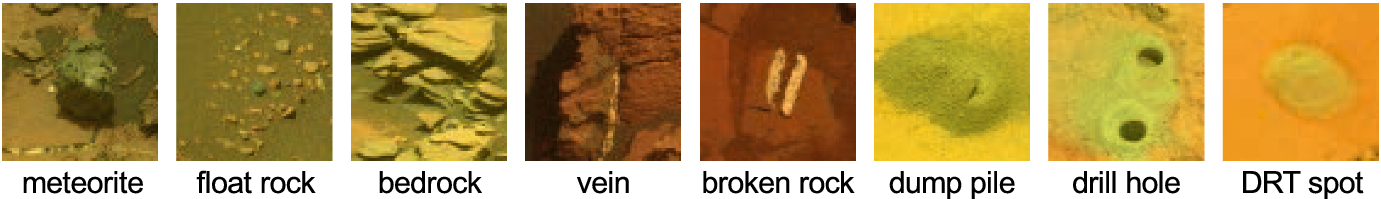
\includegraphics[width=\linewidth]{figs/1/categories.png}
\caption[Novel Geology Categories for Mastcam Multispectral Images]{\textbf{Examples from the eight categories of novel geology in the Mastcam multispectral image data set \protect\cite{kerner_data}} }
\label{chap1/fig:NovelCategories}
\end{figure*}

In this work, we created a data set of all multispectral Mastcam sequences based on the pre-processing methods outlined in the labeled Mars multispectral novelty detection data set \cite{kerner_data}.
This previous data set provided images with both \textit{typical} and \textit{novel} labels cropped from the M-100 right eye of Mastcam on MSL between sols 1 to 1666.
Each example in the data set is a 64 by 64 tile with 6 bands corresponding to 6 different filters.
The tiles were sub-sampled from larger thumbnail images of around 140 by 100 pixels in size. 
Thumbnails were used rather than full resolution sequences as they are among the first available products during tactical planning. 
Additionally, uncalibrated images were used as these data are the most readily available in the tactical analysis timeline. 
To generate the data set, these thumbnails were loaded as single band images in OpenCV before combining them to produce a single, six band, tile \cite{opencv_library}.

While we did not explicitly use the labeled Mars multispectral novelty detection data set in this work, we utilized the novelty classes to verify the system.
The data set provided a set of novel tiles divided into 8 sub-classes: meteorite, float rock, bedrock, vein, broken rock, dump pile, drill hole, and DRT spot, as shown in Figure \ref{chap1/fig:NovelCategories}. 
Multispectral analysts from the Mastcam operations team identified novel geology in images using bounding boxes based on operations experience and past publications of high interest targets (e.g., \cite{wellington2017visible}).
Sub-sampled tiles that intersected with these bounding boxes were included in the novel data set.
%Multispectral analysts were tasked with drawing bounding boxes around novel features in thumbnail sequences based on their knowledge of high interest targets supported by literature.
%After cropping the thumbnails into tiles, a set of novel tiles was created from tiles containing these bounding boxes.

% The typical tile set was created by selecting images and image regions not containing a bounding box. 
% The tiles were split at the source thumbnail level into training, validation, and test sets using an 80\%/10\%/10\% split (resulting in 9302 training, 1386 validation, and 856 test tiles) while the novel tiles were used exclusively in the test set. 
% Tiles were split based on their source thumbnail to ensure tiles from the same base sequence were not included in multiple data sets, which would increase the correlation between these datasets which should be as independent as possible.

The goal of this work is to triage tactical analysis time by prioritizing interesting images and highlighting features that are otherwise difficult to identify in multispectral sequences.
While our system should be able to identify novelties such as large veins and broken rocks, which are relatively easy for analysts to identify in RGB or single-band images, highlighting these examples will not reduce tactical analysis time as much as other features that are difficult or impossible to see without detailed analysis of multispectral sequences. 
%they can be easily seen without a novelty detection system.
%Many of the examples in the original training set contain novelties that a tactical operations staff member could easily spot. 
%These examples are visible in the RGB images and do not require a novelty detection system to draw attention to them.
The Kerner et al. \cite{kerner2020comparison} data set did not account for these operational priorities when evaluating novelty detection performance. 
In order to fully evaluate the benefit of our novelty detection system in tactical operations, we created a new data set using the same pre-processing as the Kerner et al. data set. 
Instead of separating the images into typical and novel data sets, we included all multispectral sequences from the left and right eyes of Mastcam in an unsupervised manner.
The images in this data set were pre-processed in the same way as the original data set but kept as full size thumbnails instead of tiles in order to provide detections at the same resolution as they are viewed by operations staff. 
Starting with every thumbnail taken by Mastcam, the data set was filtered by sequences containing 7 different filters: RGB (no filter) and 6 narrow-band spectral filters.
Additionally, sequences containing the calibration tool were omitted. 
This filtering resulted in about 900 total sequences split between the left and right eye. 
The six narrow-band sequences were used as inputs into the algorithm and the RGB is was used for reference.
%%%%%%%%%%%%%%%%%%%%%%%%%%%%%%%%%%%%%%
\section{Methods}
%%%%%%%%%%%%%%%%%%%%%%%%%%%%%%%%%%%%%%
In this work, we employed a the pixelwise RX method for novelty scoring.
Pixelwise RX is a distribution-based method that calculates the distance between each pixel in a test image and a background distribution, which can be visualized at the image level as a heatmap of novelty scores. 
In comparison with other methods used in Kerner et al. \cite{kerner2020comparison}, pixelwise RX is out-performed when identifying images with certain types of novelties such as float rocks, veins, bedrock, and broken rock, but performs better for other novel categories. 
While this may seem like RX is a poor choice for novelty detection, the novelty scores in Kerner et al. were aggregated to image-level scores and did not compare algorithms on the basis of their ability to highlight novel pixels in an image in a way that is useful for tactical planners. 
Pixelwise RX may not have the highest performance for all types of novelty, but its scores and their associated visualizations are relatively simple and interpretable compared to other methods. 
This is an important characteristic in method selection for analysts using novelty detection methods in a tactical operations setting. Thus, we chose to use pixelwise RX for developing novelty-based tactical planning products. 
%Of the novelty detection methods discussed in previous work, algorithms that are sensitive to spectral novelties are most desirable. 
%Spectral novelties are novelties occurring due to unexpected differences in the spectrum of an object and not from the actual shape of the object.
%Methods to detect structural novelties typically pick out features visible in standard RGB images. 
%As the goal of this system is to identify novelties that are not easily observable in the uncalibrated sequences, finding structural novelties is not necessary. 
%While hard to spot structural novelties do exist, we have chosen to focus on spectral novelties as these tend to be more difficult to spot visually. 

In this study, we chose to focus on spectral novelties that are difficult for analysts to spot because they require analysis across multiple filters to find correlations difficult to identify when looking at each image separately. 
%The method chosen to detect spectral novelties is pixel-wise RX as previous work has shown it is best suited for identifying novelties with spectral differences when compared with CAEs, GANs, and PCA \cite{kerner2020comparison}.
While methods not based on novelty detection exist that help identify spectral novelties, they require calibrated data which are often unavailable during the tactical time frame. 

Unlike the other algorithms considered, RX is not a reconstruction based method for detecting novelties.
Instead, RX computes a background distribution from typical examples and compares this distribution to infer the novelty of pixels in new images \cite{reed1990adaptive}.
For novelty detection in Mastcam sequences, the background is computed using the spectrum from each pixel in all sequences in order to generalize the entirety of the data set. 
For a multispectral image with $n$ filters, the background distribution is defined by the $n \times 1$ mean spectrum vector, $\boldsymbol{\mu}$, and an $n \times n$ covariance matrix, $\boldsymbol{\Sigma}$, of all pixels in the training set \cite{guo2016anomaly}.
This provides a mean for each multispectral band and a covariance matrix for the band pairings. 
To infer the novelty in a new image, $\boldsymbol{X}$, an RX score is calculated for each $n \times 1$ pixel vector, $\boldsymbol{x}_i \in \boldsymbol{X}$, using the Mahalanobis distance between the background and the filter response values as shown in Equation \ref{chap1/eq:RX_eq}.
\begin{equation}
    \label{chap1/eq:RX_eq}
    \text{RX}(\boldsymbol{x}_i) = (\boldsymbol{x}_i - \boldsymbol{\mu})^T \boldsymbol{\Sigma}^{-1} (\boldsymbol{x}_i - \boldsymbol{\mu})
\end{equation}
This score will be referred to as the pixel novelty score as it is a measure of how novel a pixel is relative to the background distribution. 
As this method is pixel based, the dimension size of the sequence does not matter so inferences can be run on sequences of any resolution.
This is particularly useful for Mastcam as the height of each sequence of images varies. 

After computing the RX background distribution using typical sequences, Equation \ref{chap1/eq:RX_eq} can be applied to new sequences to identify novel features.
Each sequence can be analyzed individually or relative to other sequences based on their pixel novelty scores. 
To reduce the effect of brightness in the novelty scoring, separate models were created using a data set where the RGB image of the sequence is loaded as a gray scale image and used to divide the other six images in the input. 
Individual sequence analysis is accomplished by visualizing the pixel novelty scores as a heat map. 
Analysts can quickly review these heat maps to identify the most novel regions within a sequence relative to all prior sequences. 
To compare the novelty of different sequences, statistics can be calculated for each sequence and sorted.
This can help prioritize which multispectral sequence to review first. 
%%%%%%%%%%%%%%%%%%%%%%%%%%%%%%%%%%%%%%
\section{Results}
%%%%%%%%%%%%%%%%%%%%%%%%%%%%%%%%%%%%%%
%Using the training set created from all the sequences, a background distribution was created for the typical Mastcam multispectral pixel. 
%This background distribution was used to generate pixel novelty scores for each sequence in this same data set.
To assess the system's performance for the novel features in the Kerner et al. data set \cite{kerner_data}, we located the full-size thumbnails of a selection of the novel tiles from each category and verified that the novelties highlighted in the new images were self consistent with previous results in the tiles. 
The novelty detection system using pixelwise RX performs well for highlighting easy-to-spot novelties in the data set. 
Figure \ref{chap1/fig:easyNovel} shows examples of some of the easy to catch novelties that the system is able to detect. 
We claim that these examples are relatively easy for analysts to identify because the novelties they highlight can be found through careful analysis of a single RGB image.
In the first example, a broken rock is shown near the center of the image.
The novelty heat map highlights the broken rock well as well other broken rocks in the area as shown by the yellow regions.
The second example shows veins which are highlighted well in its corresponding heat map. 
By just looking at the RGB thumbnail, an untrained analyst could likely spot something novel in the image. 
Finally, the last image shows a dump pile.
This example is clearly visible in the RGB, but would also be easy to identify because the dump pile was created by the rover, so operations staff will undoubtedly be aware of its presence in the sequence. 
While these examples are novel and interesting, they are not the type of novelty that a tactical operations staff member is likely to miss, though highlighting these examples may help to pick them out of a large set of downlinked images. 

%Highlighting these examples may help to pick them out of a large set of downlinked images but the analysis is unnecessary for individual analysis.
\begin{figure}
\centering
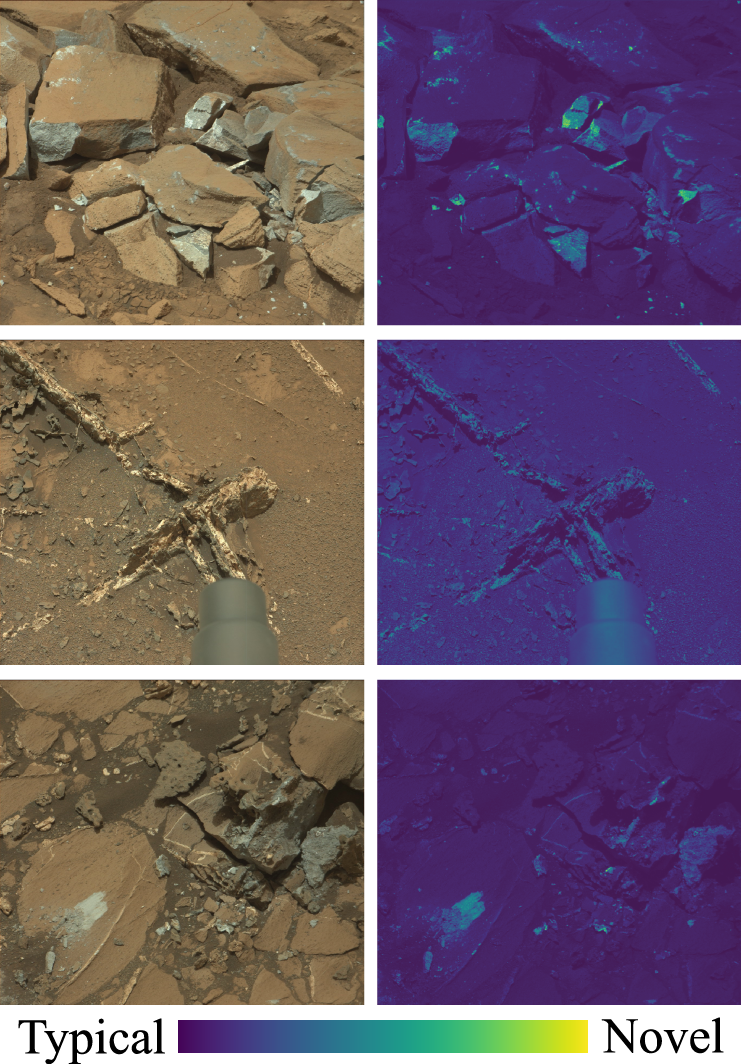
\includegraphics[width=3.25in]{figs/1/easy.png}\\
\caption{Examples of pixel novelty scores using RX for easy to spot novelties. The left column shows the RGB image from the sequence and the right column shows the output from RX with a color bar ranging from typical to novel. From top to bottom: \mbox{Broken Rock (mcam05168)}, \mbox{Veins (mcam04817)}, \mbox{Dump Pile (mcam04892)}}
\label{chap1/fig:easyNovel}
\end{figure}

To assist tactical operations planning, the novelty detection system is most useful when it is able to highlight features of interest that are not otherwise easily identifiable. 
Figure \ref{chap1/fig:mcam12276} shows an example of such a sequence.
In this sequence, there is a ring of novel material around one of the rocks near the top of the thumbnail. 
This ring is almost unidentifiable in the RGB image and faint in filters L5 and L6. 
This ring is suspected by science team members to be due to a thin layer of brighter regolith deposited around the edge of the rock and not part of the rock composition.
By taking every filter into account, RX is able to identify the spectral anomaly around this rock and provide guidance for follow up analysis.

\begin{figure*}
\centering
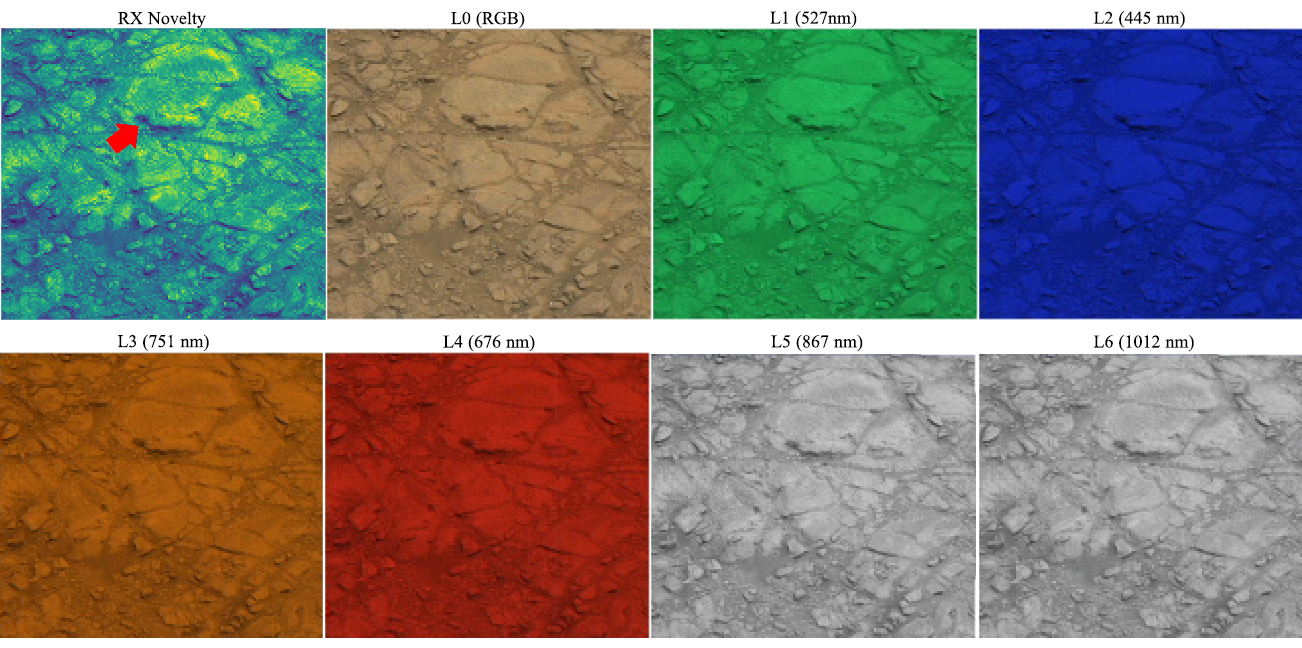
\includegraphics[width=\linewidth]{figs/1/mcam_novel.png}
\caption{\textbf{An example of difficult to notice novel features from mcam12276. In this example, there is a subtle ring of brighter dust on the edge of one of the rocks (shown by the red arrow). This is not noticeable in L0 (RGB) and faint in L5 (867 nm) and L6 (1012nm).}}
\label{chap1/fig:mcam12276}
\end{figure*}

In order to assess which sequences to analyze first, statistics about the pixel novelty scores can be calculated to rank multispectral sequences. 
Sorting by the mean pixel novelty score in each sequence orders the sequences based on mean novelty across the image.
%While the most novel sequences will rise to the top of the stack, ordering by mean pixel novelty score provides unexpected results. 
However, sorting by the mean score of all pixels in the sequence does not effectively prioritize images with obvious or localized novel features because the mean score can suppress high scores is small, localized features that are the only novel feature in the image. 
%Sequences with a high average novelty score typically consist of images without any obvious novelties as the whole image has a high average score. 
In contrast, images with high mean scores that have uniformly high scores across the entire image will not show contrast in the heat map visualization and will be difficult to interpret using this visualization. 
%This type of sorting is not fitting for tactical operations analysis as the heat map provides little useful information. 
To prioritize high novelty scores corresponding to localized features, we used the maximum pixel novelty score instead to sort novel sequences as it is better at prioritizing images with high novelty features. 
%Maximum pixel novelty score highlights sequences with clear outliers making them clearer candidates for follow up analysis. 
Examples of the top and bottom ten images sorted by maximum RX score are shown in Figure \ref{chap1/fig:sorted}. 
The top-scoring sequences show images of high variability when compared with the low-scoring images. 
The highest scoring pixel in these sequences are typically rover parts which, while being spectrally novel, are not necessarily useful for operations.
Additionally, sequences containing shadows that move over time tend to have higher scores, as the shadow fans across the different channels and creates a rainbow.
The low-scoring sequences mostly consist of sky and sand images which are relatively low interest from a tactical perspective. 
When comparing multiple images, we normalized the pixel novelty scores across the data set in order to display relative novelty. 
The scores are visualized without normalization when an analyst selects an individual sequence to analyze. 

\begin{figure*}
\centering
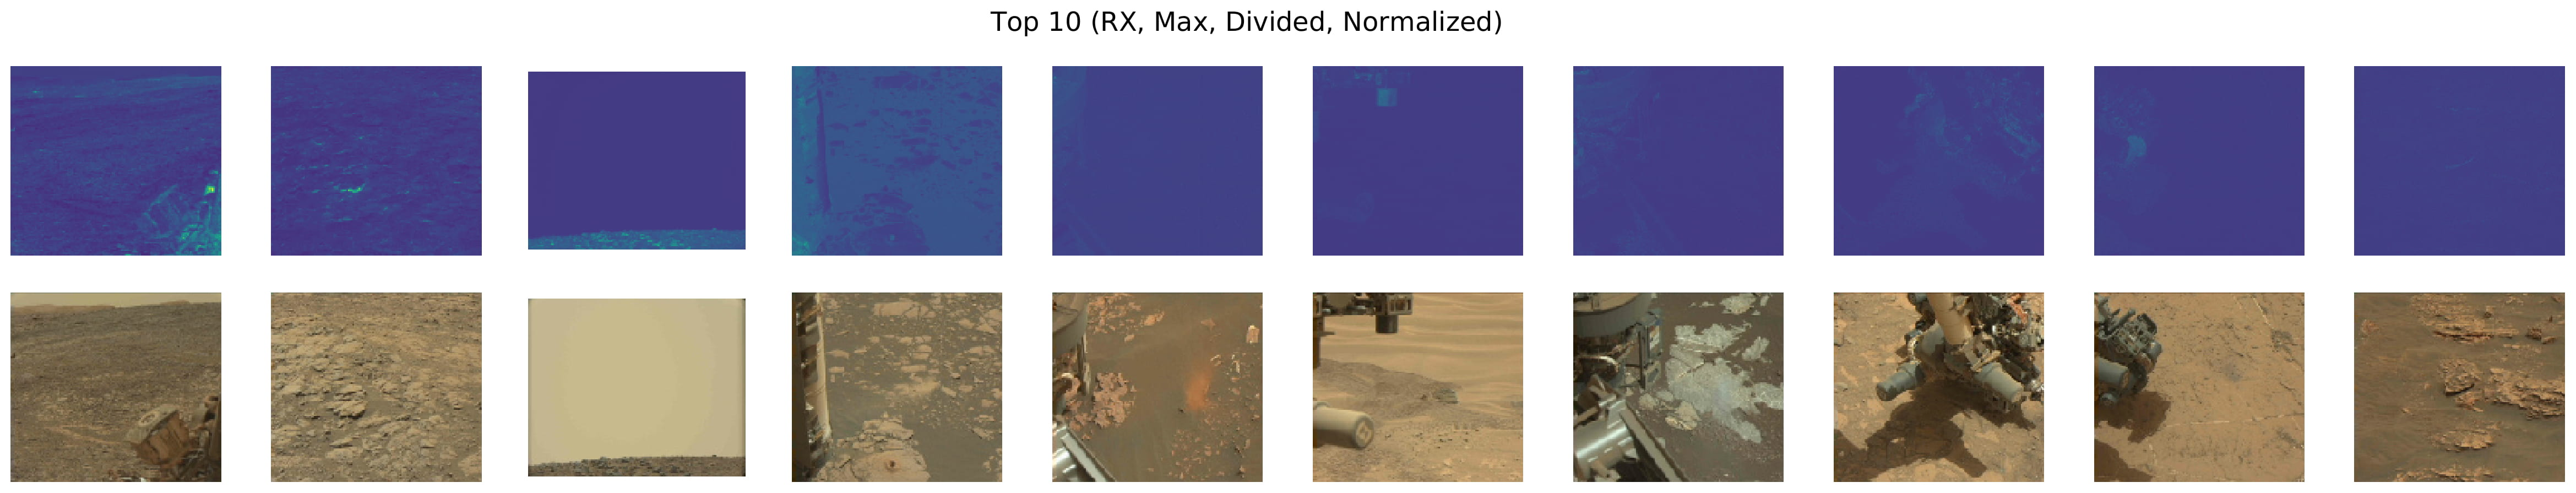
\includegraphics[width=\linewidth]{figs/1/top10.jpg}
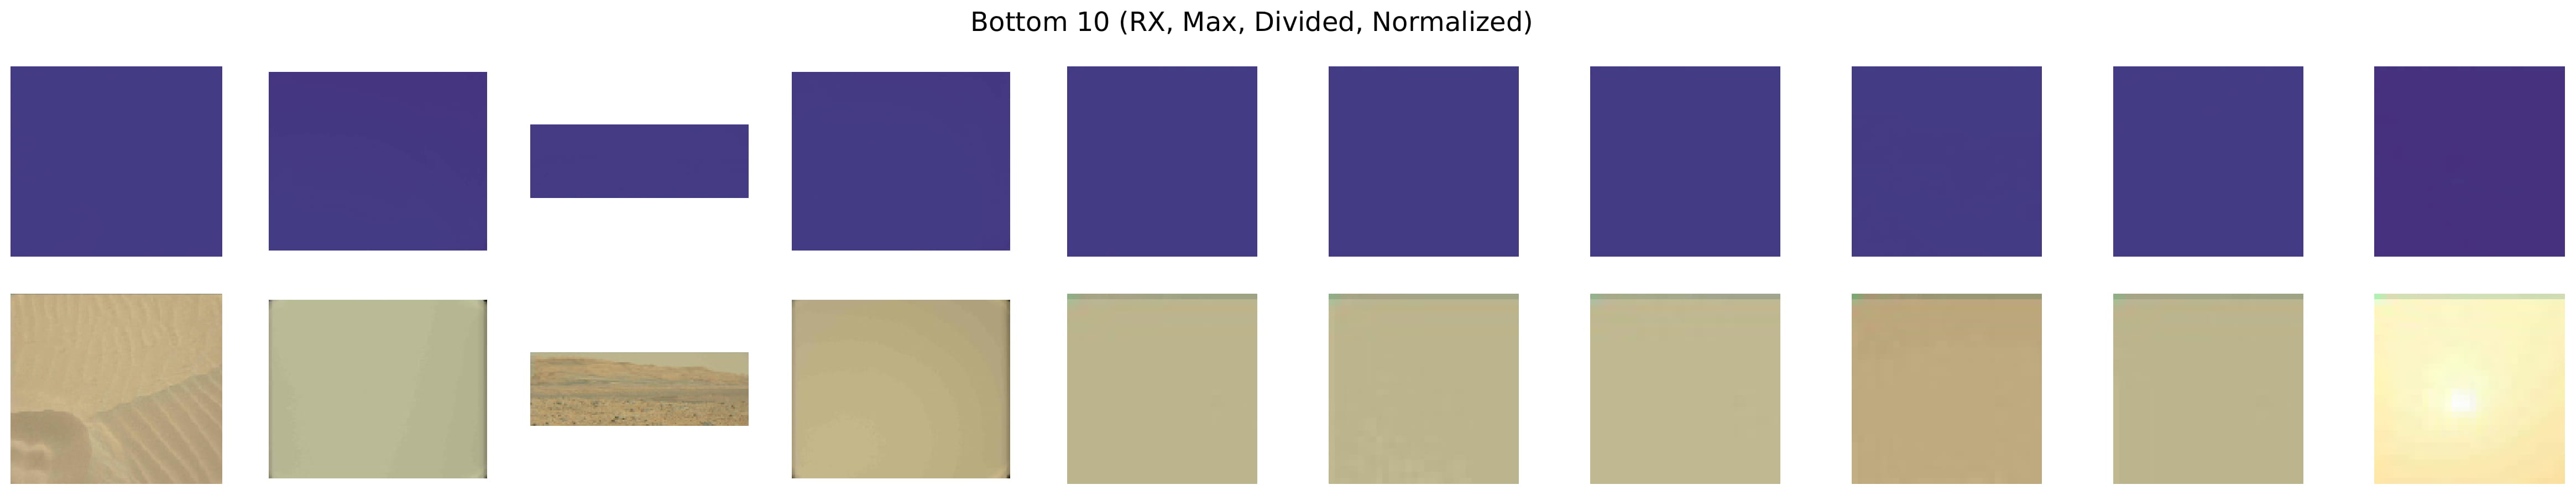
\includegraphics[width=\linewidth]{figs/1/bottom10.jpg}
\caption{\textbf{The most and least novel sequences in the Mastcam left eye data set. Sequences are sorted by maximum novelty value obtained from a brightness corrected background distribution. The pixel novelty scores  are normalized across the entire data set.}}
\label{chap1/fig:sorted}
\end{figure*}

%%%%%%%%%%%%%%%%%%%%%%%%%%%%%%%%%%%%%%
\section{Conclusions}
%%%%%%%%%%%%%%%%%%%%%%%%%%%%%%%%%%%%%%
While initial results from reviewing the novelty detection output seem promising, it is difficult to evaluate the effectiveness of the system at assisting in operations without a longer term study in which many sequences would be analyzed for previously undiscovered features.
This is necessary as generating a test set of undiscovered novelties is not feasible.
%tell the percentage of new novelties present. 
%As this study is looking for hard to detect novelties, generating a labeled test set for the undiscovered is not feasible.
The purpose of this study is to assist tactical planning so the key value is in the system's ability to highlight unique sequences and novel features within those sequences. 
The brightly colored heat map of novel regions for each sequence appears to provide a fast way of identifying spots for follow up analysis. 
The next steps for this work are to gather more feedback from the tactical planning team to determine the productivity increase while using novelty detection products.
To quantitatively evaluate this, operations staff members can be given the task of analyzing Mastcam sequence with and without the novelty-based products.
Analysis time can be recorded to identify if staff members are able to identify novel features quicker when the novelty detection system is used for triaging.
Instances where the system highlights something that the staff member does not find novel can also help to understand the limitations of the method and improve future method development.
This feedback will help to validate the usability of the novelty detection system and fine tune the features of the system, such as dividing by the brightness, global normalization, and limiting the training set to recent data. 
Additionally, the novelty detection products may improve masking rover parts and finding ways to reduce the rainbowing effect from shadows.
Another approach may be to not use a background distribution based on the entire Mastcam multispectral history and instead calculating new models for each image to find the most novel feature on a local scale.

Future work is also needed to improve ways of ordering the sequences based on their novelty scores.
While sorting sequences by the maximum pixel RX score provides more useful outputs than sorting by the mean pixel RX score, there may be better ways of prioritizing sequences (e.g., sorting by the variance of scores in the image). %heat map may help to identify sequences with spectral novelties.
To validate that the ranking's priorities align with the triage an operations staff member may perform, an experiment can also be created to have both humans and the novelty detection system generate rankings.
The rankings can be compared using Spearman's rank correlation coefficient to compare their overlap.
Such an experiment could also help to find better ways of sorting the sequences.
Finding better ways to prioritize novel sequences is also beneficial for on-board autonomy applications \cite{wagstaffnovelty}.

MSLWEB, an Arizona State University-based Mastcam tracking application, is the perfect platform for integrating novelty detection products into tactical planning workflows. 
Currently, MSLWEB supports the automatic generation of simple quick look products such as decorrelation stretches and filter ratios. 
Augmenting this system to support novelty detection would involve adding an inference endpoint to the pipeline and automatically passing new sequences through it. 
As this system is currently in use by operations staff, a strong justification is necessary to perform this integration. 
At the time, the novelty detection system has shown promising examples of novelty highlighting and sorting. 
Further analysis is needed to demonstrate how these examples would fit into the tactical planning pipeline and the time saving benefits it might provide.
\chapter[ASTHROS Payload Readout System Design]{ASTHROS Payload Readout System Design}
ASTHROS, the Astrophysics Stratospheric Telescope for High Spectral Resolution Observations at Submillimeter-wavelengths, is a balloon-borne observatory designed to study the universe in the submillimeter wavelength range.
The readout system is responsible for controlling the detectors, reading out the data, and storing the data on a solid state drive.
The readout system is designed to be modular and scalable, allowing for easy integration of new detectors and readout systems.
Each module is designed to be self-contained, focusing on a single device in the readout system so that changes to the hardware can be made without affecting the rest of the system.

\section{Raspberry Pi Compute Module 4}
From a fresh install of Raspberry Pi OS, we need to install the necessary packages to run the readout system.
The first step is to enable Secure Shell (SSH) so that we can remotely access the Raspberry Pi.
This can be done in the Raspberry Pi Configuration tool by enabling SSH in the Interfaces tab.
While we're in the interfaces tool, we can also enable SPI and Remote GPIO. 
These are necessary to interface with the PMCC.

Next, we need to configure the networking interfaces. 
\texttt{eth0} is the wired interface to the rest of the readout network. 
We need a static IP for the CM4 to ensure that other devices on the network can easily find it.
In the network settings at the top right of the screen, we can select "Edit Connections" under Advanced Options. 
From there, you will see "Wired connection 1" which is the default name for the wired interface.
Select the interface and navigate to the IPv4 Settings tab.
Chance the method from "Automatic (DHCP)" to "Manual" and add the IP address, Netmask, and Gateway.
For ASTHROS, we have the IP addresses of all CM4s set to \texttt{192.168.1.13X} where \texttt{X} is uniquely assigned to each CM4.
The Netmask is set to \texttt{23} so we can access all devices on the \texttt{192.168.1.X} readout network as well as the \texttt{192.168.0.X} gondola network.
Finally, the Gateway is set to \texttt{192.168.1.1} when attached to the gondola and \texttt{192.168.1.101} when attached to the readout network.
This is because, when connected to a test bench, we utilize the NAS as our router to access other devices on the network.
When connected in flight configuration, we disable the NAS's router functionality and use the gondola's router instead.

Next, we need to configure the SPI interface's buffer size and enable SPI on boot.
This is done by appending the following to the end of the \texttt{/boot/cmdline.txt} file:
\begin{verbatim}
    spidev.bufsiz=65536
\end{verbatim}
This sets the SPI buffer size to 64KB which is the maximum size for the PMCC.
For loading on boot, we need to add the SPI device to the \texttt{/etc/modules} file.
This is done by adding the following line to the file:
\begin{verbatim}
    spi_bcm2835
\end{verbatim}

Each of the CM4s will control up to four PMCCs, so we need to enable unique SPI busses for each PMCC.
This is done on the \texttt{/boot/config.txt} file by adding the following lines:
\begin{verbatim}
    dtoverlay=spi0-1cs
    dtoverlay=spi3-1cs
    dtoverlay=spi4-1cs
    dtoverlay=spi5-1cs
\end{verbatim}
This enables the SPI0, SPI3, SPI4, and SPI5 busses on the CM4.
While we could, in theory, only use two SPI busses and use the chip select lines to control two PMCCs on each bus, we decided to use a single chip select line for each PMCC to simplify the wiring harness and ensure our bandwidth is not saturated.

At this point, it is a good idea to reboot the CM4 to ensure that all changes have taken effect.
To verify the SPI busses are enabled, we check the \texttt{/dev} directory for the SPI devices which should be \texttt{/dev/spidevX.0} where \texttt{X} is the SPI bus number.
After rebooting and verifying the SPI has been setup, we recommend connecting the CM4 to the internet through a wireless hotspot so we can install the necessary packages.
The first package we need to install is the pigpio library.
This is a library that allows us to control the GPIO pins on the CM4.
To install the pigpio library, we need to run the following commands:
\begin{verbatim}
    sudo apt-get update
    sudo apt-get install pigpio
\end{verbatim}
After installing the pigpio library, we need to enable the pigpio daemon to run on boot.
This is done by running the following command:
\begin{verbatim}
    sudo systemctl enable pigpiod
\end{verbatim}

Finally, we need to install the actual Python packages that we will use to control the PMCC.
First we need to clone the PyMCC repository from GitHub.
This is done by running the following command:
\begin{verbatim}
    git clone https://github.com/asthros/pymcc.git
\end{verbatim}
Because this is a private repository, you will need to enter your GitHub username and personal access token.
You will need to generate a personal access token on GitHub and use that as your password when prompted.
After cloning the repository, we need to install the Python packages.
This is done by running the following command:
\begin{verbatim}
    pip3 install -r pymcc/requirements.txt
\end{verbatim}
This will install all the necessary packages to run the PyMCC module.

Finally, we need to edit the hosts file on the CM4 to ensure that we can access the other devices on the readout network by name.
This is done by updating the \texttt{/etc/hosts} file with the IP addresses and hostnames in Appendix \ref{chap2/appendix:hosts}.

\section{PMCC}
For ASTHROS, we utilize an array of 4GHz spectrometers called the PMCC ASIC P19800B ASIC RF Spectrometer, henceforth referred to as the PMCC.
These PMCCs are interfaced with via SPI for control, diagnostics, and readout \cite{PMCCP19800B}.
To communicate with the PMCCs, we utilize Raspberry Pi Compute Module 4s (CM4s) with custom harnesses.
The CM4 was chosen because it can be configured to operate at the 1.8V logic level necessary for PMCC by moving a diode on the CM4 IO board \cite{cm4io}.
Additionally, the CM4 has 4 SPI buses, allowing us to control up to 4 PMCCs per device \cite{cm4}.
The PMCCs are also connected to a GPIO pin on the CM4 to allow us to send a reset signal to the PMCCs.
The custom harness used to connect the PMCCs to the CM4 mounts onto the CM4 IO board's GPIO pins and converts the 40 ribbon cable to four sets of connections for the PMCC's SPI and reset pins.
Additionally, the CM4 has an SSD mounted to the side of it's IO board enclosure for raw spectra storage and easier local debugging when the device is not connected to the rest of the readout network.
Finally, two CM4s and eight PMCCs are mounted in a custom enclosure that is designed to be mounted on the back of the ASTHROS primary mirror.

PyMCC is the Python module developed to interface with the PMCCs and communicate with the rest of the readout system.
Originally, the PMCCs were controlled by a C program that was designed to provide a simple CLI for manually controlling the PMCCs.
As we needed to control multiple PMCCs and have them communicate with the rest of the readout system, we decided to rewrite the control software and drivers in Python.
The core of PyMCC is a Python driver for the PMCCs that provides an interface for controlling the PMCCs and reading out the data.
Built on top of the driver are Python programs that allow for manual control of the PMCCs, as well as a server that allows for control of the PMCCs over the RabbitMQ network.

\subsection{\texttt{spi\_utils}}
At the lowest level of the PyMCC driver is the \texttt{spi\_utils} module.
This module provides an interface for communicating with the PMCCs over SPI using the \texttt{spidev} Python library.
The \texttt{spidev} library provides an interface to the Linux kernel's SPI device driver \cite{spidev}.
Additionally, the PMCC has 16-bit registers that require us to send and receive 16-bit words instead of the typical 8-bit bytes that \texttt{spidev} expect. 
This was the primary reason for the development of the \texttt{spi\_utils} module as it handles the conversion between 16-bit words and 8-bit bytes and provides an easier interface for configuring the PMCCs registers without having to worry about the low-level details of the SPI communication.

The \texttt{spi\_utils} module provides a \texttt{PMCC\_SPI} class that is used to communicate with the PMCCs.
The \texttt{PMCC\_SPI} class is initialized with the bus, device, SPI mode, bits per word, and clock speed for the PMCC with which we are communicating.
The bus and device are specific to the PMCC we are communicating with and are based on the wiring harness used to connect the PMCC to the CM4.
The SPI mode, bits per word, and clock speed are all set to the values specified in the PMCC manual.

To simplify addresses, the \texttt{PMCC\_SPI} object has a \texttt{make\_addr()} method that takes the address of the register we want to write to and the read/write bit.
Valid addresses for the PMCC are 0-511, and the read/write bit is 0 for a write and 1 for a read.
When sending a command to the PMCC, the first word of the command is the address of the regster we want to write to shifted left by 1 bit to make room for the read/write bit.
\begin{equation}
    \text{tx[16]} = \text{addr[9]} << 1 + \text{rw[1]}
\end{equation}
Because \texttt{spidev} uses 8-bit communication, we need to split the 16-bit word into two 8-bit bytes.
\begin{equation}
    \label{chap2/eq:split_word}
    \text{byte[8][2]} = [\text{word[16]} >> 8,\ \text{word[16]}\ \text{\&}\ \text{0xFF}]
\end{equation}
The helper method returns these two bytes as an array that can be used in other methods to convert an address and command into a format that can be sent over SPI.

For reading and writing to the PMCC, the \texttt{PMCC\_SPI} object has an \texttt{xfer()} method that takes the address of the register, a read or write flag, and optional data to write and length of data to read.
By default, the length of data to read is 1, and the data to write is None.
The \texttt{xfer()} method first obtains the TX bytes from the \texttt{make\_addr()} method.
For both read and write commands, we utilize the \texttt{spidev} library's \texttt{xfer3()} function as it allows us to send and receive data of arbitrary length in a single SPI transaction \cite{spidev}.
\texttt{spidev}'s \texttt{xfer2()} and \texttt{xfer()} will fail at list values longer than the maximum SPI buffer size.
On the other hand, \texttt{xfer3()} will automatically split the data into multiple SPI transactions if the data is longer than the maximum SPI buffer size.
This is vital for burst reads on the PMCC as our data can be much longer than the maximum SPI buffer size.
For writes, the \texttt{xfer()} method sends the TX bytes and the data to write to the PMCC.
The data is split into two 8-bit bytes using Equation \ref{chap2/eq:split_word}.
During this transaction, the PMCC does not send any data back, so the \texttt{xfer3()} function returns an array of zeros.
If our transaction is unsuccessful, instead of returning zeroes, we will receive an empty array that we can check for.
For single register reads, the \texttt{xfer()} method sends the TX bytes followed by a dummy word to the PMCC.
While we are sending the dummy word over the MOSI line, the PMCC is sending the data we requested over the MISO line that is returned by the \texttt{xfer3()} function along with the original TX bytes.
After checking that we have received data from the PMCC, we return the data as an array of 16-bit words.
This is done by utilizing NumPy to cast the output as a \texttt{np.uint8} array and then returning a view of that array with big-endian 16-bit unsigned integer data type.
For reads that are longer than a single register, we send the TX bytes followed by a dummy word for each word we want to read and follow the same process as a single register read.

For simple reads, \texttt{PMCC\_SPI} has a \texttt{read()} method that takes the address of the register we want to read from and optionally the number of words we want to read.
By default, this method reads a single word from the PMCC.
The \texttt{read()} method calls the \texttt{xfer()} method with the read flag set to 1 and the number of words to read.
If we are only reading a single word, we return the first word and only word in the array of words returned by the \texttt{xfer()} method. 
Otherwise, for burst reads, we return the entire array of words.

Often times, we want to read a specific value over and over until that value is True.
Many status bits on the PMCC operate in this way to indicate when a specific operation has completed. 
To accomplish this, the \texttt{PMCC\_SPI} object has a \texttt{poll()} method that takes the address of the register we want to read from, the bit within the register we want to check, the amount of time to wait between reads, and the maximum number of reads.
The \texttt{poll()} method then issues a \texttt{read()} of that register and checks if the bit is set by shifting the read value to the right by the bit number and checking if the least significant bit is set.
If the value is not set, we wait for the specified amount of time and read the register again.
This process is repeated until the value is set or the maximum number of reads is reached.
We then return if the value was set or not instead of raising an exception if the value is not set.
The implementation of raising exceptions is left to the user of the \texttt{poll()} method depending on the use case.

For simple writes, \texttt{PMCC\_SPI} has a \texttt{write()} method that takes the address of the register we want to write to and the data we want to write.
The \texttt{write()} method calls the \texttt{xfer()} method with the read flag set to 0.
From there, the \texttt{xfer()} method sends the data to the PMCC and returns None as the PMCC does not send any data back.
If there is an issue with the transaction, the \texttt{xfer()} method will raise an exception indicating that it received null from the transfer to the specific address. 

The documentation for the PMCC specifies specific bits and ranges of bits within a register address to set different configurations on the device.
We often only want to change a specific value at an address and not the entire register.
To accomplish this, the \texttt{PMCC\_SPI} object has a \texttt{mask\_data()} method that takes the most significant bit (MSB), the least significant bit (LSB), the value we want to write, and the original buffer we are overwriting.
This closely matches the way the PMCC documents the use of each register with either a single bit or an inclusive range of bits. 
First we check if the MSB and LSB are valid values, and if they are not, we raise an exception.
Valid values for addressing the 16-bit registers are 0 to 15 for the LSB and LSB to 15 for the MSB.
Next, we check if the value provided will fit within the length specific by the MSB and LSB.
We then use the MSB and LSB to calculate the maximum value that will fit in the mask. 
We use this maximum value to determine if the provided value is too large, in order to raise an exception if it is.
Finally, we create a mask using the maximum value and shifting it to the left by the LSB.
We then take the original buffer and do a bitwise AND with the inverse of the mask to clear the bits between the LSB and the MSB. 
Finally, we shift our data to the left by the LSB and do a bitwise OR with the original buffer to set the bits between the LSB and MSB to the new value.
This process is shown in Equation \ref{chap2/eq:mask_data}.
\begin{align}
    \label{chap2/eq:mask_data}
    \text{maxValue} &= (1 << (\text{MSB} - \text{LSB} + 1)) - 1 & 0 \leq \text{LSB} \leq \text{MSB} \leq 15\\
    \text{mask} &= \text{maxValue} << \text{LSB} \\
    \text{buffer} &= (\text{buffer}\ \&\ \sim\text{mask})\ |\ (\text{data} << \text{LSB}) & 0 \leq \text{data} \leq \text{maxValue}
\end{align}

To further simplify the process of setting specific bits in a register, the \texttt{PMCC\_SPI} object has a \texttt{read\_write()} that first reads from the address we want to write to, modifies the data we want to change, and then writes the modified data back to the PMCC.
The \texttt{read\_write()} method takes the address of the register we want to read from and one of the following formats for the data we want to write:
\begin{itemize}
    \item A tuple of MSB, LSB, and value to write to the register 
    \begin{itemize}
        \item e.g. \texttt{(15, 8, 0xAA)} would set the register to \texttt{0b1010 1010 XXXX XXXX}
    \end{itemize}
    \item A tuple of a single bit and value to write to the registers
    \begin{itemize}
        \item e.g. \texttt{(2, 0x1)} would set the register to \texttt{0bXXXX XXXX XXXX X1XX}
    \end{itemize}
    \item An array containing combinations of the above two formats
    \begin{itemize}
        \item e.g. \texttt{[(15, 8, 0xAA), (2, 0x1)]} would set the register to \texttt{0b1010 1010 XXXX X1XX}
    \end{itemize}
\end{itemize}
The \texttt{read\_write()} method first reads the data from the PMCC using the \texttt{read()} method and stores it in a buffer.
Then we check if the changes provided are a tuple or an array of tuples.
If it's a tuple, we just wrap it in an array in order to iterate over it.
For each change in the array, we unpack the tuple and call the \texttt{mask\_data()} method to modify the data we read from the PMCC, updating the buffer each time.
If we are only changing a single bit, MSB and LSB are set to the same value.
To complete the transaction, we write the modified buffer back to the PMCC using the \texttt{write()} method.


Finally, we provide a \texttt{close()} method that simply calls the \texttt{close()} method on the \texttt{spidev} object to close the SPI connection.

\subsection{\texttt{config}}
There are a number of device specific configurations that need to be set for each PMCC in order to operate correctly.
To simplify the process of writing code to configure the PMCCs, we utilize the YAML configuration file format to store the configuration for each PMCC \cite{yaml}.
This YAML file has information about the RMQ configuration as well as spectrometer configuration. 
For now, we will focus on the spectrometer configuration and discuss the RMQ configuration in Section \ref{chap2/section:rmqtools}.
The spectrometer config section, \texttt{spec}, is split into two main sections for the PMCCs, global variables used for every spectrometer, and spectrometer specific variables.
For each experiment, we would like to have a single configuration file that can be used on every CM4 to configure multiple PMCCs. 
To accomplish this, each CM4 is given a unique name that we use to differentiate between each device. 
Each PMCC connected to a CM4 is then indexed, so we can individually address each one by specifying the CM4 name and the PMCC index.

The format for the global configurations is shown in Table \ref{chap2/table:pmcc_config}.
These configurations are used to set values we don't expect to individually change for each PMCC.
While we may create different configurations for different experiments, such as integration time and magnitude or power mode, we will likely make these changes to all PMCCs at once and not individually.

\begin{table}[h!]
    \centering
    \begin{tabularx}{\textwidth}{l|l|X}
        \textbf{Key} & \textbf{Type} & \textbf{Description} \\ \hline    
        \texttt{spec\_file} & string & Path to the spectrometer hardware file \\
        \texttt{int\_time} & int & Integration time in milliseconds \\
        \texttt{clock\_freq} & int & Reference clock frequency in MHz \\
        \texttt{resolution} & int & 16 or 32 for 16-bit or 32-bit readout resolution \\
        \texttt{shift} & int & 0 or 4 for 0 or 4 bit shift \\
        \texttt{magnitude} & bool & True for magnitude mode, False for power mode \\
        \texttt{window\_bypass} & bool & True to enable rectangular window bypass \\
        \texttt{window\_bit\_growth} & bool & True to enable window div 2 bypass \\
        \texttt{butterfly\_shift} & bool & True to enable butterfly shift for improved noise measurements \\
        \texttt{wiring} & array & See Table \ref{chap2/table:wiring} for wiring configuration \\
        \texttt{groups} & dict & Dictionary of CM4 names and an array of PMCC chip IDs  \\
    \end{tabularx}
    \label{chap2/table:pmcc_config}
    \caption{Global Variables in the PMCC Configuration File}
\end{table}

After the global configurations, an array of four spectrometer wiring configurations is provided. 
In full operation, we will have four PMCCs connected to each CM4, so we need a way of specifying the wiring for each PMCC's SPI bus and GPIO reset pin.
Because the harness is identical for each CM4, we can specify the wiring for each PMCC along the harness, and it will be the same for every CM4. 
The only exception to this is the lone 100GHz PMCC connected to its own CM4. 
The wiring for this PMCC is simply the first index in the wiring array will still work with the rest of the system.
Each item in the wiring configuration is as follows in Table \ref{chap2/table:wiring}.

\begin{table}[h!]
    \centering
    \begin{tabularx}{\textwidth}{l|l|X}
        \textbf{Key} & \textbf{Type} & \textbf{Description} \\ \hline    
        \texttt{dev} & string & Path to device address (e.g. \texttt{/dev/spidev0.0}) \\
        \texttt{gpio} & int & GPIO pin number for the reset signal\\
        \texttt{speed} & int & SPI device speed in Hz, typically 5000000 unless changes for stability reasons and debugging\\
    \end{tabularx}
    \label{chap2/table:wiring}
    \caption{Wiring Configuration in the PMCC Configuration File}
\end{table}

Finally, we have the group configuration dictionary. 
Each PMCC comes with a chip ID specified by the manufacturer used to set pre-calibrated values, such as the ADC time skew.
The configuration dictionary consists of a CM4 name as the key and an array of PMCC chip IDs as the value.
This allows us to specify which PMCCs are connected to each CM4 and configure them accordingly.
For the 100GHz PMCC and CM4, the array will only contain a single chip ID.

When loading in the configuration file, we create a \texttt{PMCC\_Config} object that all configuration information necessary for the CM4. 
We initialize this object with the \texttt{spec} part of the YAML file, the group name of the CM4, and an array of PMCC indexes to configure (e.g. \texttt{[1, 2, 3, 4]} for all spectrometers).
The \texttt{PMCC\_Config} object then creates properties for each of the global configurations that can be accessed by the \texttt{PMCC\_SPI} object.
We set the resolution mode of the PMCCs using the \texttt{resolution} and \texttt{shift} properties and a lookup table for the proper register values as shown in Table \ref{chap2/table:resolution}.
We could, theoretically, set higher values for LSB shift but for the purposes of ASTHROS, we only need 0 and 4 bit shifts.

\begin{table}
    \centering
    \setlength{\extrarowheight}{2pt}
    \begin{tabular}{cc|c|c|}
      & \multicolumn{1}{c}{} & \multicolumn{2}{c}{Resolution}\\
      & \multicolumn{1}{c}{} & \multicolumn{1}{c}{\texttt{16-Bit}}  & \multicolumn{1}{c}{\texttt{32-Bit}} \\\cline{3-4}
      \multirow{2}*{LSB Shift}  & $0$ & \texttt{0x080} & \texttt{0x0C0} \\\cline{3-4}
      & $4$ & \texttt{0x180} & \texttt{0x1C0} \\\cline{3-4}
    \end{tabular}
    \caption{Resolution Mode Configuration for PMCC}
    \label{chap2/table:resolution}
\end{table}

After the global variables are loaded, we create a dictionary of device configurations for individual PMCCs. 
This dictionary is indexed by the CM4 group name concatenated with the PMCC index.
Each value in the dictionary is a \texttt{PMCC\_Device\_Config} object that is initialized with the chip ID, the wiring configuration at the PMCC index, and the \texttt{spec\_file} for configuration.
The wiring information is paired with the chip ID to create a \texttt{PMCC\_Device\_Config} object that can later be used to configure the PMCC. 
The provided \texttt{dev} path for the SPI configuration is split and stored into the bus and device number for the \texttt{PMCC\_SPI} object to use.
Finally, the pre-calibrated values are loaded from the \texttt{spec\_file} by searching for the chip ID in the file and storing the associated values in the \texttt{PMCC\_Device\_Config} object.
If the chip is not found in the file, we raise an exception that the configuration provided was not valid. 
The final product is a \texttt{PMCC\_Config} object that contains all the necessary information to configure both the CM4 and any number of PMCCs connected to it. 

\subsection{\texttt{consts}}
The \texttt{consts} module is simply a collection of constants used throughout the PyMCC module.
Many of these are register addresses so that we can easily reference them in the code without having to go back and forth between the PMCC manual and the code.
Additionally, we have some large arrays that are used in configuration that we don't want to hard code into the code.
For example, \texttt{WINDOW\_COEFFS} is a vector of 513 values used to configure the symmetrical 1024 point FFT on the DSP. 
In addition to addresses and coefficients, we keep an array of default values for the PMCC registers so that we can easily identify issues with the device after reset. 

\subsection{\texttt{driver}}
The \texttt{driver} module is the highest level of the PyMCC module and is responsible for providing all functionality for the PMCCs. 
Each PMCC is controlled by a \texttt{PMCC\_Driver} object that is initialized with a \texttt{PMCC\_Config} object and the index of the spectrometer in the config that we want to control.
After initializing the object, the user must call the \texttt{initialize\_interface()} method to setup a \texttt{PMCC\_SPI} object to communicate with the PMCC.
Following SPI setup, the user must call the \texttt{initalize\_gpio()} method to setup the GPIO pin for the reset signal.
Both of these methods check the wiring configuration in the \texttt{PMCC\_Config} object to ensure that the correct wiring is provided.
With both of these methods called, the \texttt{PMCC\_Driver} object is ready to start the PMCC configuration. 

The first thing done before any configuration is toggling the reset signal on the PMCC.
This is done by calling the \texttt{reset()} method with a boolean value to set the reset signal high followed by low.
\texttt{reset()} is often called multiple times in the configuration process to ensure that the PMCC is in a known state before configuring it.

\begin{quote}
    \textbf{Note:} The PMCC documentation specifies individual bit fields for each register. 
    When referring to a specific register in the documentation, we will use the format \texttt{reg\_name} with lowercase letters. 
    These will be identical to the register names in the documentation. 
    During the development of PyMCC, we often had to refer to SPI addresses that contain multiple PMCC registers. 
    When referring to these addresses, we will use the format \texttt{REG\_NAME} with all uppercase letters.
    These are not documented in the PMCC manual but are used to reference addresses defined in the \texttt{consts} module.
\end{quote}

After resetting the PMCC, we need to calibrate the Phase Lock Loop (PLL) on the PMCC using \texttt{initialize\_pll()}.
The PLL is used to synthesize all required clocks for the PMCC with the use of an external reference clock. 
Initializing the PLL is done in three steps, resetting the PLL with \texttt{reset\_pll()}, calibrating the PLL with \texttt{calibrate\_pll()}, and finally loading the ADC with the PLL values using \texttt{load\_adc()}.
\texttt{reset\_pll()} resets the PLL and sets the ADC gain, offset, and time skew configurations. 
This is done by the following sequence of commands:

\begin{enumerate}
    \item 
        Write to the \texttt{CHIP\_CONF} to reset the DSP.
    \item 
        Read and write the \texttt{PLL\_LOCK\_CONF} to set the \texttt{lock\_desired\_count} to 3, \texttt{lock\_tune\_off} to 2, and \texttt{lock\_tune\_on} to 4. 
        These set the lock detector control that will later be used to determine if we have locked the PLL.
    \item 
        Read and write the \texttt{PLL\_FVCO\_CAL\_CONF} to set the \texttt{fvco\_cal\_settletime} to 4. 
        This is used by the PLL's Voltage Controlled Oscillator (VCO) to determine the settling time for the VCO.
        By setting this to 4, we are setting our settle time to $2^{4} = 16$ times the reference frequency.
    \item 
        Read and write the \texttt{ADC\_GAIN\_ACCUM} and set the \texttt{adc\_gain\_cal\_accum} to 3 which sets the on-chip gain calibration accumulator length to 8192. 
    \item 
        Read and write the \texttt{ADC\_GAIN\_CONF} and set the \texttt{adc\_gain\_cal\_settle} to 3 which adjusts the delay during the gain calibration to 63 clock cycles. 
    \item 
        Read and write the \texttt{ADC\_OFFS\_CONF} and set the \texttt{adc\_offs\_cal\_accum} to 3 and the \texttt{adc\_offs\_plr} to 1. 
        This sets the on-chip offset calibration accumulator length to 8192 and the polarity of the offset calibration to fine (comparator) adjustment mode. 
    \item 
        Read and write the \texttt{ADC\_TIME\_SKEW\_COEF} to set the \texttt{time\_skew\_select} to 0xF. 
        This enables the use of manual time skew codes for the ADC.
    \item 
        Finally, write to the \texttt{DEMUX\_DEL\_ADJ\_A} to \texttt{DEMUX\_DEL\_ADJ\_D} to adjust the delay in the input interleaver clock for the four ADC groups. 
        This value is set to 11 for all four registers, setting the delay to $18.8*11 = 206.8$ ps. 
        Currently, this step is hard coded to 206.8 ps but, in the future, we may want to adjust this value based on the chip ID as these values are pre-calibrated for each chip.
\end{enumerate}

After resetting the PLL, we calibrate the PLL using \texttt{calibrate\_pll()}.
This takes many of the values we set in \texttt{reset\_pll()} to execute the calibration process. 
The calibration process is as follows:

\begin{enumerate}
    \item 
        Check if the clock frequency set in the configuration is a multiple of 2000. 
        Clocks must be a factor of 2GHz to ensure that the PLL can lock to the reference clock.
    \item 
        Read and write to the \texttt{PLL\_CONF} and set the \texttt{pll\_freq\_adjust} and the \texttt{pll\_ndiv}. 
        The \texttt{pll\_freq\_adjust} is used to set the sampling rate of the ADC. 
        We set this value to 2 which indicates a 4GHz clock for the ADC. 
        The \texttt{pll\_ndiv} is used to set the divider ratio for the PLL feedback. 
        This value is calculated using $N_{div} = 2000 \text{MHz} / F_{freq}$ and set in the \texttt{pll\_ndiv} register. 
        For our 100 MHz reference clock, we set the \texttt{pll\_ndiv} to 20.
    \item 
        Now we begin the calibration process by reading and writing to the \texttt{PLL\_FVCO\_CAL\_CONF} to set the \texttt{fvc\_cal\_start} to 1 and resetting the \texttt{fvco\_cal\_settletime} to 4. 
        This starts the calibration process and sets the settling time to 16 times the reference frequency.
    \item 
        Finally, we poll the \texttt{fvco\_cal\_cal\_done} bit until the band selection is completed. 
        If the calibration is not completed after a default of 10 retries, we raise an exception indicating that the PLL calibration failed.
\end{enumerate}

After the PLL is calibrated, we load the ADC with the PLL values using \texttt{load\_adc()}.
Many of the commands sent during this set are writes instead of reads and writes.
This is because we actually want to override the registers are not setting to 0.
The process for loading the ADC is as follows:
\begin{enumerate}
    \item 
        Write to the \texttt{VGA\_CURRENT\_CONF} to set the \texttt{vga\_current\_out\_adjust} and \texttt{vga\_offset\_rng}.
        The \texttt{vga\_current\_out\_adjust} is used to adjust the reference current at the VGA output buffer from 2.1 to 6.3 mA in steps of .6 mA.
        We set this to $2.1 + 6 * .6 = 5.7$ mA by setting the value to 6.
        The \texttt{vga\_offset\_rng} is used to adjust the offset compensation reference current from 250 to 600 uA in steps of 50 uA.
        We set this value to $250 + 7 * 50 = 600$ uA by setting the value to 7.
    \item 
        Write to the \texttt{VGA\_GAIN\_CONF} to set the \texttt{vga\_peak\_cntrl} and \texttt{vga\_gain\_adjust}.
        The \texttt{vga\_peak\_cntrl} is used to reduce the inductive AC peak of the VGA by increasing the capacitance.
        We set this value to a code of 5.
        The \texttt{vga\_gain\_adjust} is used to adjust the VGA gain from 0 to 10.4 dB in steps of approximately .53 dB.
        We set this value to $8 * .53 = 4.24$ dB by setting the value to 8.
    \item 
        Write to the \texttt{VGA\_CONFIG} to enable the common-mode compensation (\texttt{vga\_cm\_comp}), the VGA offset compensation (\texttt{vga\_offset}), and the VGA enable (\texttt{vga\_en}).
        These values are all defaulted to enabled, but it is good practice to set them to ensure that the VGA is properly configured.
    \item 
        Write the four \texttt{adc\_time\_skew\_adjust1} to \texttt{adc\_time\_skew\_adjust4} registers to set the time skew for the ADC.
        These values are pre-calibrated for each chip and are set in the \texttt{PMCC\_Device\_Config} object.
    \item 
        Write to the \texttt{ADC\_TIME\_SKEW\_CONF} to set the \texttt{time\_skew\_mode}, \texttt{time\_skew\_select} and \texttt{time\_skew\_polarity}.
        The \texttt{time\_skew\_mode} is set to 1 to enable calibration for a configured time instead of continuous calibration.
        The \texttt{time\_skew\_select} is set to 0b1111 to enable each of the four time skew adjustments.
        The \texttt{time\_skew\_polarity} is set to 1 to enable inverse polarity of the time skew code adjustment direction.
    \item 
        Write a 0 to \texttt{adc\_rst\_n} to register a reset to the ADC.
    \item 
        Write a 0 to \texttt{adc\_sub\_clk\_gen\_rst\_n} to reset the clock generators for all four ADC groups.
    \item 
        Sleep for 100 ms to allow the ADC to reset.
    \item 
        Write a 1 to \texttt{adc\_rst\_n} to enable the ADC.
    \item 
        Write a 1 to \texttt{adc\_sub\_clk\_gen\_rst\_n} to enable the clock generators for all four ADC groups.
\end{enumerate}

After those three steps, the PLL is calibrated and the ADC is ready for configuration.
To verify this, the \texttt{PMCC\_Driver} object has a \texttt{check\_connection()} method that checks if we can read from the PMCC.
We first read the \texttt{CHIP\_ID} register to ensure that we can communicate with the PMCC.
Despite having the same name as the chip ID we use to differentiate between PMCCs, the \texttt{CHIP\_ID} register is a fixed value that is set by the manufacturer and will always be 0x6 for the second generation 4GHz PMCCs.
Reading the \texttt{CHIP\_ID} register is a good way to verify that SPI connection is working.
We then read the \texttt{PLL\_LOCK\_LOL} register to determine if we have a Loss of Lock (LOL) on the PLL.
If the PLL is locked, the \texttt{PLL\_LOCK\_LOL} register will be 0.
If we make it past both of these checks, we return True to indicate that the PMCC is connected and the PLL is locked.

The usual next step in the configuration process is to calibrate the gain and offset of the ADC. 
This is done by calling the \texttt{calibrate\_adc()} method.
This method is a wrapper for the \texttt{calibrate\_adc\_offset()} and \texttt{calibrate\_adc\_gain()} methods and runs both of them twice.
The calibrations run in interactive mode so running them twice allows the PMCC to iterate on the calibration values and get a more accurate result.
To run the offset calibration, we set the following values within the \texttt{ADC\_OFFS\_CONF} register:

\begin{itemize}
    \item \texttt{adc\_offs\_cal\_en} to 1 to enable the offset calibration
    \item \texttt{adc\_offs\_cal\_mode} to 1, setting the operation mode to a zero offset calibration.
    \item \texttt{adc\_offs\_cal\_interactive} to 1 to start a new calibration using the previous adjustment codes. 
\end{itemize}

After setting these values, we poll the \texttt{adc\_offs\_cal\_ack} bit until the calibration is complete.
For the gain calibration, we simply have to set the \texttt{adc\_gain\_cal\_en} to 1 to enable the gain calibration.
We then poll the \texttt{adc\_gain\_cal\_ack} bit until the calibration is complete. 
After both calibrations are run twice, we are done calibrating the ADC. 

In the instance we already know the values we want to set for the gain and offset, we provide a \texttt{calibrate\_adc\_preset()} method that takes arrays of the 23 gain and 23 offset values to set the calibration values.
These values are loaded into the 23 \texttt{ADC\_REF\_ADJUST\_XX} and 23 \texttt{ADC\_OFFS\_ADJUST\_COMP\_XX} registers respectively.
The \texttt{adc\_gain\_cal\_mode} and \texttt{adc\_offs\_cal\_mode} registers also need to bet set to 0x1 and 0x2 to enable the use of the preset values.

After calibrating the ADC, we are able to configure the DSP. 
This is highly subjective to the experiment being run but, for ASTHROS, we have a specific configuration that we use that works for the integration time and resolution we are using. 
In future version of the code, we will likely pull out some of the hard coded values and make them configurable in the YAML file.
The configuration process is as follows:
\begin{enumerate}
    \item Reset the DSP by writing a 1 to the \texttt{CHIP\_CONF} register's \texttt{dsp\_reset}.
    \item Load the window coefficients into the DSP by writing the 513 values in the \texttt{WINDOW\_COEFFS} array to the \texttt{WINDOW\_REGISTER} register one at a time followed by a pulse to the \texttt{dsp\_coeff\_dest\_wind} bit to shift store the value and shift the register.
    \item 
        Write to the \texttt{dsp\_skip\_fft\_stage} register to 0 to use all four stages of the FFT. 
        This results in 512 frequency bins per sub-band. 
    \item 
        Write to the \texttt{DSP\_READOUT\_CONF} with the mode from the configuration file as shown in Table \ref{chap2/table:resolution}. 
        This sets the resolution and shift for the readout.
    \item 
        Write to the \texttt{CHIP\_CONF} register to set the \texttt{dsp\_enable} bit to 1 to enable the DSP and \texttt{dsp\_acc\_mode} to 1 to enable continuous FFT operation. 
    \item 
        Read and write to the \texttt{FFT\_CONFIG} to set the \texttt{dsp\_magn\_bypass}, \texttt{dsp\_wind\_bypass}, \texttt{dsp\_div\_red\_wind}. 
        These values are set in the configuration file and are used to enable the magnitude or power mode, the windowing function, and window bit growth. 
    \item 
        Calculate the number of integrations to run based on the integration time. 
        We do this by diving our desired integration time by the length of time it takes to run a single accumulation on the DSP. 
        For the ADC running at 8 GS/s (Gigasamples per second) reading 16384 time domain bins, this number is 2.048 us.
        The number of accumulations we collect per integration is a 24-bit value split across two registers. 
        The 16 most significant bits are stored in the \texttt{dsp\_acc\_num\_msb} register and the 8 least significant bits are stored in the \texttt{dsp\_acc\_num\_lsb} register.
    \item 
        If we are in power accumulation mode, we need to set the data shift for the DSP. 
        The maximum output resolution is <40 bits so we need to shift the data to the right depending on the integration time.
        We calculate this by taking the binary logarithm of the number of accumulations per integration and subtracting 8.
        We get eight because there is a maximum output resolution of 40 bits and the most we can shift the value is 32.
        By subtracting 8 from the binary logarithm, we get the number of bits we need to shift the data to the right that would maximize the output resolution without overflowing the readout.
        This value is then stored in the \texttt{dsp\_data\_shift} register.
    \item 
        If we are using a butterfly shift, we set the data divide by 2 blocks to the following values:
        \begin{itemize}
            \item \texttt{dsp\_bfly\_shift\_pfb} to \texttt{0b10101} to alternate between enabled and disabled IFFT processor stages. 
            \item \texttt{dsp\_bfly\_shift\_fft} to \texttt{0b1010101010} to alternate between enabled and disabled FFT processor stages.
        \end{itemize}
        The combination of these essentially skips every other stage of the IFFT and FFT processor, increasing performance for band-limited noise measurements.
        It accomplishes this by skipping the stages that would divide the data by 2 to reduce the risk of overflow. 
    \item 
        Write to the \texttt{VGA\_CURRENT\_CONF} to set the \texttt{vga\_current\_out\_adjust} and \texttt{vga\_offset\_rng}.
        We set these values to the same values as we did in the ADC calibration.
    \item 
        Finally, we perform a \texttt{check\_connection()} to ensure everything is in order and return the status.
\end{enumerate}

At this point, the PLL has been locked, the ADC has been calibrated and the DSP has been configured. 
The most common next step is to start the DSP and begin acquiring data. 
This is done in two parts, pulsing the accumulation bit and then reading the data. 
Pulsing the accumulation bit is done in the \texttt{pulse\_acquisition()} method by writing a 1 to the \texttt{dsp\_start\_acc} register.
This starts the DSP's operation and begins accumulating data.
After starting accumulation, we immediately perform a single \texttt{retrieve\_data()} to clear any garbage data that may be present in the DSP's output buffer.

The \texttt{retrieve\_data()} method follows the following process to read a spectra from the DSP:
\begin{enumerate}
    \item 
        Read the \texttt{dsp\_data\_ready} register to determine if the DSP has finished accumulating data.
        We poll this register at a rate of 500 Hz for a maximum of 2000 retries. 
        Both of these values are adjustable agruments to this method but are set to 500 Hz and 2000 retries by default.
        If we don't recieve data after the maximum number of retries, we raise an exception indicating that the DSP did not finish accumulating data.
        Otherwise, we continue to the next step.
    \item 
        Write a pulse to the \texttt{dsp\_start\_readout} register to start the readout process. 
    \item  
        Take a timestamp to record the time the readout started.
    \item 
        Start the readout process by performing a burst read of the \texttt{DSP\_READOUT\_ADDRESS} at \texttt{0x4000}. 
        If we are performing a 32-bit readout, we read the address 8193 times to get the first half of our data. 
        Otherwise, for a 16-bit readout, we read the address 8192 times.
    \item 
        If we are performing a 32-bit readout, we read the second half of the data by reading the \texttt{DSP\_READOUT\_ADDRESS} at \texttt{0x8000} 8191 times.
        This strange number of reads is due to a bug that causes issues if reading two 8192 blocks of data.
        Without following this specific sequence, we will be missing one value in the second half of the data, shifting the entire readout. 
    \item 
        Regardless of the resolution, we write a pulse to the \texttt{dsp\_reset\_ready} register to begin the next accumulation.
        This discards any data that may be present in the readout buffer so that new data can be stored. 
    \item 
        Finally, we return the data and the timestamp to the user. 
        If the resolution is 32-bit, we concatenate the two arrays and use NumPy to return a view of the data as an array of 32-bit unsigned integers.
        Otherwise, for 16-bit readouts, we use NumPy to return a view of the data as an array of 16-bit unsigned integers.
\end{enumerate}

Another common operation after setup is to read raw data from the ADC. 
This can be useful to ensure that the ADC is working correctly by measuring the mean and swing of the digitized signal. 
The \texttt{retrieve\_adc()} method does just this using the following procedure. 
\begin{enumerate}
    \item Write a 0 to the \texttt{dsp\_reset} register and a 1 to the \texttt{dsp\_enable} to enable the DSP.
    \item Write a 0 to the \texttt{dsp\_proto\_en} to disable prototype mode on the ADC.
    \item Write a 0 to the \texttt{DSP\_DEBUG\_MODES} to clear any other debug modes that may be enabled.
    \item Write a 1 to the \texttt{debug\_wr\_from\_adc} register at the \texttt{DSP\_DEBUG\_MODES} address to begin writing ADC samples into the debug buffer. 
    \item Begin polling the \texttt{debug\_wr\_from\_adc\_done} register to determine when the ADC samples have been written to the debug buffer. If we reach the maximum number of retries, we raise an exception that the ADC data was not ready after the maximum number of retries.
    \item Write a 0 to the \texttt{DSP\_DEBUG\_MODES} to disable writing the ADC samples to the debug buffer.
    \item Write a 1 to the \texttt{debug\_wr\_by\_spi} register at the \texttt{DSP\_DEBUG\_MODES} address to begin moving the debug buffer to the SPI readout buffer.
    \item Finally, we perform single reads of the \texttt{ADC\_READOUT\_ADDR} at \texttt{0x2000} until we have read all 16384 samples in sets of 8 words across the 2048 lines in the ADC. 
    To convert these values into the actual readout from the 20 ADC cores, we have to do quite a bit of bit manipulation. 
    This is because each of the 20 core's readout is a 6-bit value split across the 8 words in the line. 
    Accomplishing this is done by the following steps:
    \begin{enumerate}
        \item Start with an array of 8 16-bit words that contain the 20 6-bit for cores A to T. \\
        {\raggedright 
        \texttt{RRRRSSSSSSTTTTTT OOPPPPPPQQQQQQRR MMMMMMNNNNNNOOOO JJJJKKKKKKLLLLLL GGHHHHHHIIIIIIJJ EEEEEEFFFFFFGGGG BBBBCCCCCCDDDDDD XXXXXXXXAAAAAABB}
        \par}
        \item Take the array of 8 words and reverse the order. The first word from the readout contains the least significant bits of the line. \\ 
        {\raggedright
        \texttt{XXXXXXXXAAAAAABB BBBBCCCCCCDDDDDD EEEEEEFFFFFFGGGG GGHHHHHHIIIIIIJJ JJJJKKKKKKLLLLLL MMMMMMNNNNNNOOOO OOPPPPPPQQQQQQRR RRRRSSSSSSTTTTTT}
        \par}
        \item Convert the array of 8 16-bit words into an array of 16 8-bit bytes. \\
        {\raggedright
        \texttt{XXXXXXXX AAAAAABB BBBBCCCC CCDDDDDD EEEEEEFF FFFFGGGG GGHHHHHH IIIIIIJJ JJJJKKKK KKLLLLLL MMMMMMNN NNNNOOOO OOPPPPPP QQQQQQRR RRRRSSSS SSTTTTTT}  
        \par}
        \item Unpack the 8-bit bytes into their binary bits using NumPy's \texttt{unpackbits()} method. \\
        {\raggedright
        \texttt{
            XXXXXXXXAAAAAABBBBBBCCCCCCDDDDDDEEEEEEFFFFFFGGGGGGHHHHHH-
            IIIIIIJJJJJJKKKKKKLLLLLLMMMMMMNNNNNNOOOOOOPPPPPPQQQQQQRR-
            RRRRSSSSSSTTTTTT
            }
        \par}
        \item Throw away the first 8 bits of the output as these are used for padding the data.\\
        {\raggedright
        \texttt{
            AAAAAABBBBBBCCCCCCDDDDDDEEEEEEFFFFFFGGGGGGHHHHHHIIIIIIJJJJJJ-
            KKKKKKLLLLLLMMMMMMNNNNNNOOOOOOPPPPPPQQQQQQRRRRRRSSSSSSTTTTTT}
        \par}
        \item Reshape the array of bits into an array of 20, 6-bit values. \\
        {\raggedright
        \texttt{AAAAAA BBBBBB CCCCCC DDDDDD EEEEEE FFFFFF GGGGGG HHHHHH IIIIII JJJJJJ KKKKKK LLLLLL MMMMMM NNNNNN OOOOOO PPPPPP QQQQQQ RRRRRR SSSSSS TTTTTT}
        \par}
        \item Pack the 6-bit values back into 8-bit bytes using NumPy's \texttt{packbits()} method. This method adds zero padding to the end of the array if the length is not 8. \\
        {\raggedright
        \texttt{AAAAAAXX BBBBBBXX CCCCCCXX DDDDDDXX EEEEEEXX FFFFFFXX GGGGGGXX HHHHHHXX IIIIIIXX JJJJJJXX KKKKKKXX LLLLLLXX MMMMMMXX NNNNNNXX OOOOOOXX PPPPPPXX QQQQQQXX RRRRRRXX SSSSSSXX TTTTTTXX}        
        \par}
        \item Right shift the 8-bit bytes by 2 to remove the padding added by the previous step.\\
        {\raggedright
        \texttt{AAAAAA BBBBBB CCCCCC DDDDDD EEEEEE FFFFFF GGGGGG HHHHHH IIIIII JJJJJJ KKKKKK LLLLLL MMMMMM NNNNNN OOOOOO PPPPPP QQQQQQ RRRRRR SSSSSS TTTTTT}
        \par}
    \end{enumerate} 
    \item Perform this process for all 2048 lines in the ADC readout.
    \item Compute the mean and standard deviation of the ADC lines. 
    \item Compute the swing of the ADC using the mean and standard deviation. 
    \begin{equation}
        \text{Swing} = \sigma * 2\sqrt{2}
    \end{equation}
    \item Return the buffer of ADC readouts, the mean, the standard deviation, and the swing.
\end{enumerate}

% The next method in the \texttt{PMCC\_Driver} object is the \texttt{prbs_test()} method.
% The PRBS is the Pseudo-Random Binary Sequence that can be injected into readout data to test the system.
% % We use this method to test the LVDS readout which we never use so I don't know why we have this method???


Finally, we provide two methods to read and write to all of the PMCC registers. 
These methods are \texttt{fetch\_registers()} and \texttt{write\_registers()}.
There are 512 different SPI addresses that can be read and written to on the PMCC.
This method allows us to dump the current state of the PMCC or set the PMCC to a known state.
These are mostly used for debugging and are not used in the normal operation of the PMCC.

\subsection{\texttt{data\_utils}}
\texttt{data\_utils} provides a few handy classes to handle storing data from the PMCC. 
The simplest of these is the \texttt{PMCC\_Register\_Writer} which, as the name suggests, is able to write the PMCC registers to a file. 
This is useful for debugging and for storing the state of the PMCC for later use.
This class is initialized as an object with a path to the directory where the data will be stored.
Using this object, we can call the \texttt{write\_registers()} method with an array of register values to write the data to a CSV. 
The data in the CSV will include the register address, the integer value, the hex value, and the default hex value for each register. 
The file is saved with a timestamp in the filename, so we can identify when the file was written. 
The \texttt{PMCC\_Register\_Writer} object also has a \texttt{read\_registers()} method that reads the data from the CSV and returns an array of register values that could be used to set the PMCC to the state it was at when the snapshot was taken. 
Finally, there is a simple \texttt{get\_files()} method that returns all the files in the directory where the data is stored.

We also provide a \texttt{PMCC\_ADC\_Writer} class that is used to write the raw data from an ADC test. 
This class is initialized with a path to the directory where the data will be stored.
The \texttt{write\_adc()} method is called with the data from the \texttt{retrieve\_adc()} method from \texttt{PMCC\_Driver} and writes the data to a CSV.
This results in 2048 lines of data with the 20 values for each core in each line.
The file is saved with a timestamp in the filename, so we can identify when the test was done. 

Finally, we have our spectra writers. 
We need to support writing in both HDF5 and CSV formats.
HDF5 will be used during the flight to store the data in a more efficient format, whereas CSV is used for debugging and testing.
For writing to HDF5, we provide the \texttt{PMCC\_H5\_Spectra\_Writer} class.
This class takes in a path to the directory where the data will be stored, a reference to the spectrometer's driver, the maximum number of writes before the file is closed, and the data type of the spectra. 
In initialization, we create the directory if it does not exist. 
We also start a counter at 0 to keep track of the total number of spectra written by the writer. 

Before writing the data, we need to create the HDF5 file using the \texttt{new\_file()} method.
If a file is already linked to the writer, we closed that file and open a new one.
Next, we create a new file with \texttt{spec\_<prefix>\_<timestamp>.h5} as the filename.
\texttt{prefix} is an optional paramater that can be used to identify the file and \texttt{timestamp} is the current time.
The file is created with two datasets. 
The first dataset is called \texttt{stamps} and is used to store the timestamps of the spectra.
The second dataset is called \texttt{data} and is used to store the spectra.
Both datasets are created using the \texttt{gzip} compression filter with a compression level of 4.
This is done to reduce the size of the file and speed up the writing process. 
The shape of these datasets is determined by the \texttt{max\_writes} parameter and the length of the spectra.
The \texttt{stamps} dataset is a 1D array of 64-bit doubles with a length of \texttt{max\_writes}.
The \texttt{data} dataset is a 2D array with a shape of \texttt{max\_writes} by the length of the spectra and a data type matching the specified data type during initialization.
A header is added to the \texttt{data} dataset and contains the attributes shown in Table \ref{chap2/table:h5_header}.
After creating the file, we start a counter at 0 to keep track of the number of spectra in the file. 

\begin{table}[h!]
    \centering
    \begin{tabularx}{\textwidth}{l|X}
        \textbf{Attribute} & \textbf{Description} \\ \hline    
        \texttt{id} & Name of the the spectrometer (\texttt{<CM4\_name><PMCC\_index>}) \\
        \texttt{chip} & PMCC Chip ID from manufacturer \\
        \texttt{int\_time} & Integration time (ms) \\
        \texttt{resolution} & 32 or 16-bit data resolution \\
        \texttt{shift} &  0 or 4 for 0 or 4 bit shift \\
        \texttt{magnitude} & True if magnitude mode is enabled, False if power mode is enabled \\
        \texttt{window\_bypass} & True if window bypass is enabled \\
        \texttt{window\_bit\_growth} & True if window bit growth is enabled \\
        \texttt{butterfly\_shift}  & True if butterfly shift is enabled\\
    \end{tabularx}
    \caption{Attributes of the \texttt{data} dataset in the HDF5 file}
    \label{chap2/table:h5_header}
\end{table}

When writing data to the file, we use the \texttt{write\_spectra()} method.
This method takes in a timestamp and the spectra to write to the file.
If the file does not exist, or we have reached a maximum number of writes, we rerun the \texttt{new\_file()} method to create a new file.
We then write the timestamp and spectra to the \texttt{stamps} and \texttt{data} datasets at the current index.
After writing the data, we increment the count of spectra in the current file and the total count of spectra written by the writer.

The \texttt{PMCC\_CSV\_Spectra\_Writer} class is used to write the data to a CSV file.
It is almost identical to the \texttt{PMCC\_H5\_Spectra\_Writer} class but writes the data to a CSV file instead of an HDF5 file.
The \texttt{PMCC\_CSV\_Spectra\_Writer} also implements \texttt{write\_spectra()} and \texttt{new\_file()} methods so that they it be used interchangeably with the \texttt{PMCC\_H5\_Writer} class.
For \texttt{new\_file()}, the file is created with the name \texttt{spec\_<prefix>\_<timestamp>.csv} and no header is written to the file.
Just like the \texttt{PMCC\_H5\_Spectra\_Writer}, the \texttt{PMCC\_CSV\_Spectra\_Writer} will close the previous file if one exists and start a new counter for the number of spectra in a file when a new file is created.
The \texttt{write\_spectra()} method concatenates the timestamp and the spectra and writes them to the file as a single line.
This method also increments the count of the number of spectra in the file, the total number of spectra written by the writer, and will create a new file if one doesn't exist or we reach the maximum number of spectra in a file.

Finally, we provide a wrapper class called \texttt{PMCC\_Spectra\_Writers} that takes in an array of \texttt{PMCC\_H5\_Spectra\_Writer} and \texttt{PMCC\_CSV\_Spectra\_Writer} objects.
This class is used to write data to multiple files at once. 
This is useful for writing data to both HDF5 and CSV files at the same time as well as data to multiple locations, such as locally on the CM4 and remotely on the NAS. 
\texttt{new\_file()} and \texttt{write\_spectra()} simply call the same methods on all of the writers in the array.
This wrapper also keeps track of the total number of spectra written which is useful for housekeeping and telemetry.                      %   \include rather than \input for chapters
\chapter[On-Board Science Data Quality Analysis using Anomaly Detection for ASTHROS]{On-Board Science Data Quality Analysis using Anomaly Detection for ASTHROS}
\section{Abstract}
ASTHROS (Astrophysics Stratospheric Telescope for High Spectral Resolution Observations at Submillimeter-wavelengths) is a high-altitude balloon mission utilizing an array of sixteen spectrometers to create high spatial resolution 3D maps of ionized nitrogen gas in galactic and extragalactic star-forming regions.
During data collection, we utilize on-the-fly mapping, where the instrument continuously collects spectra while scanning over a target area.
After a sweep across the target, we take a calibration spectra to correct our science data.
These calibration spectra provide a baseline for how the instrument is operating at a given moment.
As we collect new calibration spectra, we can compare the current calibration with a series of past calibrations to determine if our system is producing anomalous spectra.
Some examples of anomalous spectra are changes in RFI spike frequency, location, or amplitudes, changes in the overall readout level, and changes in the shape of the spectra.
We compare statistical and data-driven methods for detecting these anomalies and evaluate their performance to determine the best fit for the ASTHROS readout system. For data-driven methods, we compare the latent space representation of our calibration spectra with past calibrations using models like Variational AutoEncoders (VAE) and Principal Component Analysis (PCA).
By comparing with a rolling window of past calibrations, we allow our system to change gradually while identifying sudden irregularities.
When spectra are labeled as anomalous, they are prioritized for review so that the ground operations team can analyze and address the issue.
On-board analysis is enabled by the readout system architecture which utilizes the RabbitMQ (RMQ) messaging networking.
RMQ allows us to modularly build our readout system and create additional functionality, such as on-board analysis, without making modifications to the operation pipeline. 


\section{Introduction}
ASTHROS (Astrophysics Stratospheric Telescope for High Spectral Resolution Observations at Submillimeter-wavelengths) is a high-altitude ballooning mission utilizing an array of sixteen spectrometers to create high spatial resolution 3D maps of ionized nitrogen gas in galactic and extragalactic star-forming regions \citep{siles2020asthros}. 
On-the-fly (OTF) mapping will be employed during data collection where each spectrometer will continuously produce ON and OFF spectra as we scan across our target as show in in Figure \ref{chap3/fig:scan} \citep{mangum2007fly}. 

\begin{figure}[h]
    \centering
    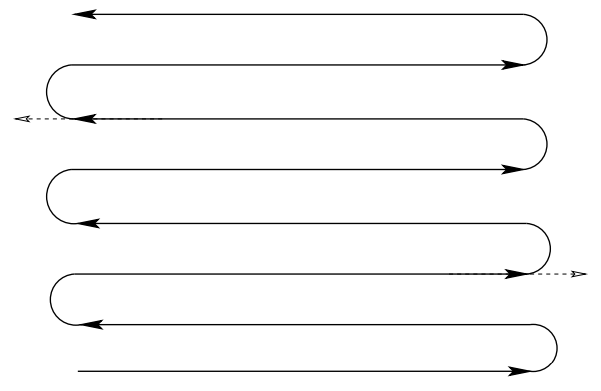
\includegraphics[width=0.5\linewidth]{figs/3/scan.png}
    \caption{An example scanning pattern for OTF mapping. ASTHROS will continuously produce ON spectra while scanning across the target and OFF spectra when observing a calibration source from \cite{mangum2007fly}.}
    \label{chap3/fig:scan}
\end{figure}

Once data collection has started, our spectrometer array will continuously produce and timestamp spectra and save the raw time stream to itself and a separate storage device. 
The clocks of all the computers on board ASTHROS will be synchronized using a local NTP server such that the timestamps can be harmonized with pointing data from the gondola to label ON and OFF spectra \citep{mills1991internet}.
After a sweep across the target, we will find spectra taken during the OFF segments and use them to evaluate our system's performance.
By generating an anomaly score for these calibrations, we can determine if our system is behaving differently than expected when compared to a series of past calibrations.

Currently, the methods for evaluating system performance are done on the ground by checking spectra manually as they come down.
This is an error-prone process as it is difficult to manually check each calibration spectrum for anomalies.
By implementing on-board anomaly detection, we can automate this process and prioritize analysis of anomalous spectra for review by the ground operations team.
This will allow us to quickly identify and address any issues with the system during flight to catch errors while we're still able to correct them instead of waiting until the end of the mission to find out that our data is unusable.
Even if the anomaly detection system is not perfect, any form of quantifiable measure of science data quality will be an improvement over the current manual process.


This paper will focus on the on-board analysis of our calibration spectra to detect anomalies in the system.
Section \ref{chap3/sec:system} will go over the system architecture for ASTHROS and how we can utilize RabbitMQ (RMQ) to enable on-board analysis.
After that, Section \ref{chap3/sec:methods} will discuss the methods we used to detect anomalies in our calibration spectra.
Then, in Section \ref{chap3/sec:data}, we will discuss the data we used to evaluate our methods and how we collected the data.
Section \ref{chap3/sec:results} will present the results of our analysis and conclude which method is the best fit for the ASTHROS readout system.
Finally, Section \ref{chap3/sec:future} will discuss future work for implementation on ASTHROS. 

\section{System Architecture}
\label{chap3/sec:system}
The ASTHROS readout system is composed of three main computers that respectively handle commanding the instrument, storing science data, and analyzing our telemetry and science data. 
Our goal with this readout system is to be able to collect and analyze data in real time so that any changes in detector behavior can be quickly identified and addressed during flight. 
To achieve this, we utilize RabbitMQ (RMQ) to create a modular system that can be easily expanded to include additional functionality by creating a standard protocol for Remote Procedure Calls (RPC) and Publish/Subscribe (Pub/Sub) messaging \citep{dobbelaere2017kafkaversusrabbitmq}.
RMQ is a lightweight messaging broker based communications to seamlessly create a network of computers that are able to share status and commands between multiple concurrent systems \citep{thompson2024architecture}.

\begin{figure}
    \centering
    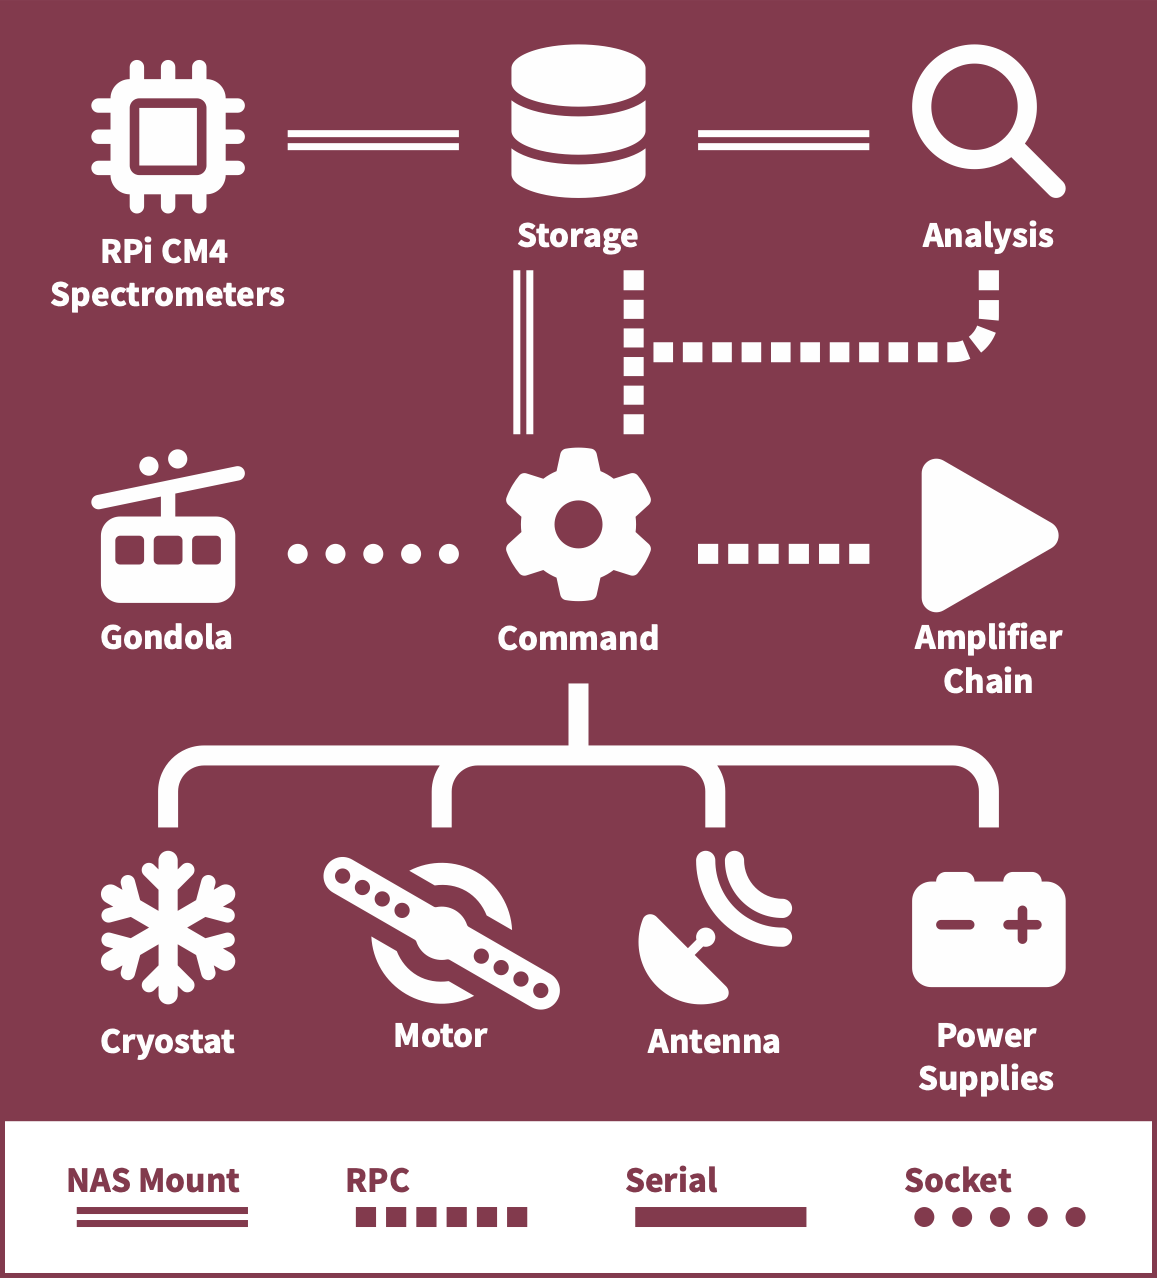
\includegraphics[width=0.5\linewidth]{figs/3/system.png}
    \caption{A high level overview of the ASTHROS Readout Network System Architecture showing the Command, Storage, and Analysis computers. The Command computer is responsible for sending commands to other processes and receiving status updates from the various publishers on the RMQ network. The Storage computer is responsible for storing all science data and telemetry data collected during the flight. The Analysis computer is responsible for analyzing the science data collected during the flight. The overview also shows some of the various subsystems and how they're connected in the network.}
    \label{chap3/fig:system}
\end{figure}

The core of ASTHROS's readout are three systems: the Command, Storage, and Analysis computers as shown in Figure \ref{chap3/fig:system} \citep{horton2024readout}.
The Command computer is responsible for sending commands to other processes and receiving status updates from the various publishers on the RMQ network. 
This computer also manages telemetry through a connection to the gondola. 
Key system devices, such as the power supplies and the antenna, are connected directly to this computer via serial connections to allow for real-time monitoring and control.
Despite being physically on the same computer, control of each of these subsystems is handled by separate processes that communicate with the Central process through RMQ.
This allows any of these processes to be moved to a different computer or replaced with a new process without changing the overall system architecture.
As most of the systems are located on the Command computer, we host the RMQ broker on this computer to minimize latency and reduce the number of network hops between the Command computer and the other systems.

The Storage computer is responsible for storing all science data and telemetry data collected during the flight.
This computer is a custom-built rugged Network Attached Storage (NAS) that is able to store all the data collected during the flight.
This NAS houses 4 Solid State Drives in a RAID 10 configuration \citep{chen1994raid}.
Other computers on the network, such as the Command computer and the Analysis computer, are able to mount the storage computer as a network drive to read and write data.
Additionally, this storage computer has two managed network switches that allow for networking to every system on ASTHROS.
Our spectrometers, controlled by Raspberry Pi CM4s, are connected to this computer via Ethernet and are able to store their data locally on their own Solid State Drives and send a copy to the storage computer.
We do this for redundancy in case the storage computer fails during flight.

Finally, we have the Analysis computer which is responsible for analyzing the science data collected during the flight. 
This computer has the critical task of analyzing the calibration spectra to determine if the system is behaving as expected by measuring data quality. 
The methods described in this paper are run on this computer and are able to communicate with the Command computer to prioritize analysis of anomalous spectra via telemetry.
Like other computers on the network, the Analysis computer is able to mount the storage computer as a network drive to read and write data.
Using RMQ, the analysis computer is able to listen to the status exchange for pointing updates from the gondola.
If the pointing data indicates that the telescope is observing a calibration source, the Analysis computer will pull the most recent calibration spectra from the storage computer and compare it to a series of past calibrations to determine if the system is behaving as expected.
In addition to it's primary function of analyzing science data, the Analysis computer is also able to run additional processes to prepare data for the science team. 
It does this by time harmonizing the science data with the pointing data from the gondola to label each spectra with the correct pointing information so that it may be used for mapping. 

Apart from the main three computers, the ASTHROS readout system also consists of a set of Raspberry Pi Compute Module 4s (CM4s) that control the spectrometers and a set of Arduino Nano Every microcontrollers that control the amplifier chains. 
Both of these are configured to communicate over the RMQ network for Command and Control and produce status updates over the Status Exchange. 
The CM4s are responsible for controlling the spectrometers and collecting the raw time stream data from the spectrometers \citep{mohammed2024digital}.
The Arduinos are responsible for controlling the amplifier chains to adjust attenuation values for our variable attenuators \citep{Ricardo}.

\section{Methods}
\label{chap3/sec:methods}
Anomaly detection, also known as outlier detection, is a way of finding out-of-distribution data points in a dataset \citep{kerner2022domain}.
This works by comparing a data point to typical examples from the dataset and determining if the data point is significantly different from the rest of the data.
Because of the nature of anomalies, we can't use traditional supervised learning methods to detect them as we don't have labeled examples of what an anomaly looks like \citep{horton2021integrating}.
In other words, we don't fully know what we don't know and, instead of training our system on known issues, we need to train our system to recognize when something is different from what it has seen before.
To do this, we need to use unsupervised learning methods that learn the underlying structure of our data and determine if a new data point is significantly different from the rest of the data.
Figure \ref{chap3/fig:examples} shows examples of the types of anomalies we have seen in past missions. 
Typically, these anomalies present themselves as changes in RFI spikes, the shape of the readout spectra, or the overall readout bias level.

\begin{figure}[h]
    \centering
    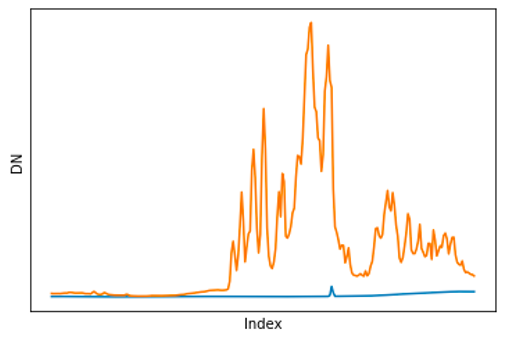
\includegraphics[width=0.3\linewidth]{figs/3/Anom1.png}
    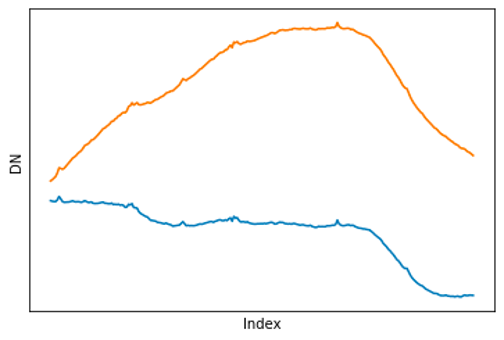
\includegraphics[width=0.3\linewidth]{figs/3/anom2.png}
    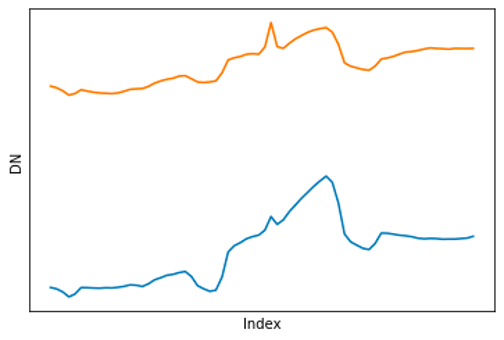
\includegraphics[width=0.3\linewidth]{figs/3/anom3.png}
    \caption{Examples of anomalous spectra from past missions. From left to right, we see changes in RFI spike shape and location, changes in the shape of the spectrum, and changes in the readout bias level.}
    \label{chap3/fig:examples}
\end{figure}

For this implementation, we focus on two methods for determining if a calibration spectrum is anomalous: Variational AutoEncoders (VAE) and Principal Component Analysis (PCA).
Both have their strengths and weaknesses and we will compare their performance on the ASTHROS calibration spectra to determine which is the best fit for our system.

\subsection{Variational AutoEncoders}
VAEs are a class of AutoEncoders that learn the mean and variance of the latent space of the data \citep{kingma2013auto}.
This is done by training the model to encode the input data into a lower dimensional space and then decode it back to the original input.
We selected VAEs for this task because they are able to learn the underlying structure of the data and generate new examples of the data by sampling from the latent space.
This is useful for anomaly detection as we can compare a new spectrum to the reconstructed spectrum to determine if it is significantly different from the rest of the data.
When a new spectrum is input into the VAE, the encoded and then decoded spectrum will be different from the original spectrum if the new spectrum is anomalous.

The architecture for our VAE is a simple feedforward neural network with multiple layers.
Our encoder consists of an input layer, a hidden layer, and two output layers for the mean and variance of the latent space.
The input layer has $8192$ nodes, one for each channel in our calibration spectra.
The hidden layer has $256$ nodes which feeds into our output layer which has $64$ nodes of mean and variance.
We re-parameterize the mean and variance to sample from the latent space and feed this into the decoder which has the same architecture hidden layer and input layers as the encoder but in reverse.
The output layer of the decoder has $8192$ nodes to reconstruct the original spectrum.

To train the VAE, we have to normalize our spectra to values between $0$ and $1$.
We then split our data into a training and testing set and train the VAE on the training set.
We then use the VAE to encode the testing set to it's latent space representation and decode it to produce a reconstructed version.

To generate an anomaly score from this method, we take a test spectrum, transform it using the VAE to it's latent space representation, and then decode the spectrum to produce a reconstructed version.
This reconstruction is imperfect as the VAE model is fit to our typical spectra.
We compare the reconstruction to our original spectrum to calculate error from the difference between the two specra.
This score can be used as a time series of anomaly scores to determine if a new spectrum is significantly different from the rest of the data. 
For flight, we will have to retrain the VAE on a subset of the data to account for changes in the system over time making more challenging for implementation.

\subsection{Principal Component Analysis}
PCA is a method that reduces the dimensionality of a dataset by finding the directions of maximum variance in the data \citep{wold1987principal}.
This is done by finding the eigenvectors, called principal components, of the covariance matrix of the data and projecting the data onto these eigenvectors.
The first principal component is the direction of maximum variance in the data, the second principal component is the direction of maximum variance orthogonal to the first principal component, and so on.
Because our calibration spectra are high dimensional with $8192$ channels, we use PCA to reduce the dimensionality of our data to a lower dimensional space where we more easily compare the spectra.

To use PCA for anomaly detection, we first fit the PCA model to a series of past calibration spectra.
This can be done in two ways, fitting the PCA model to a subset of the spectra in an entire dataset and using a rolling window of past spectra to create unique fits for each additional spectrum. 
The first method can be used to determine if PCA is a good method for fitting to the dataset by seeing how many principal components are necessary to cover the variance of a typical spectrum. 
The second method can then be used in a real time setting to determine how a new spectrum compares to the recent history of previous spectra. 

To generate an anomaly score from this method, we take a test spectrum, transform it using the fit PCA model to it's latent space representation, and then inverse transform the spectrum to produce a reconstructed version. 
This reconstruction is imperfect as the PCA model is fit to our typical spectra.
We compare the reconstruction to our original spectrum to calculate the mean squared error from the difference between the two spectra. 
We use this value as our anomaly score as it provides a measure of how different a given spectrum is from previous spectra. 

\begin{figure}[b]
    \centering
    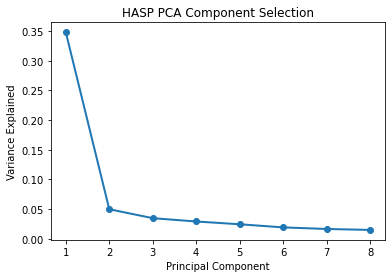
\includegraphics[width=0.49\linewidth]{figs/3/HASP_Elbow.png}
    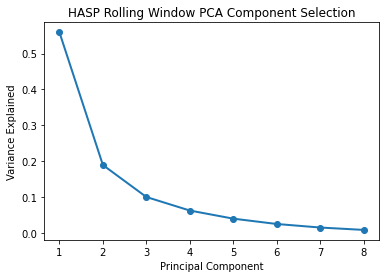
\includegraphics[width=0.49\linewidth]{figs/3/elbow.png}
    \caption{Elbow plots for the HASP dataset. Left shows the amount of variance each component accounts for in the entire dataset and the right shows the average variance amount when using a rolling window of 10 spectra.}
    \label{chap3/fig:elbows}
\end{figure}

\section{Data}
\label{chap3/sec:data}
The data for these tests are taken from two separate data collection instances. 
The first was a High-Altitude Student Platform (HASP) flight \citep{guzik2008development} that tested one of our Pacific MicroCHIP Corp (PMCC) Spectrometers  \citep{mohammed2024digital}.
A team of students at Arizona State University test flew a spare PMCC spectrometer to measure the deuterium to hydrogen ratio in the atmosphere \citep{HADHR}.
Unfortunately, the spectrometer was not calibrated properly so many of the spectra were unusable for science. 
Additionally, due to the HASP payload's suite of student projects, we had many instances of changing RFI due to other instruments on board. 
Ironically, with all these problems, this dataset is an ideal candidate for testing the anomaly detection system as we are able to use it to evaluate good and bad spectra. 
This dataset consists of about 7,000 spectra of varied levels of noise. 

The second dataset was taken from one of our 100GHz integration tests with a flight calibrated spectrometer. 
This data is extremely stable and provides us an ideal baseline for what we expect to see during flight.
Despite being an extremely clean dataset of over 20,000 spectra, there are instances of RFI in the data that can be used to demonstrate the real time data quality assessment of the spectra. 

\begin{figure}
    \centering
    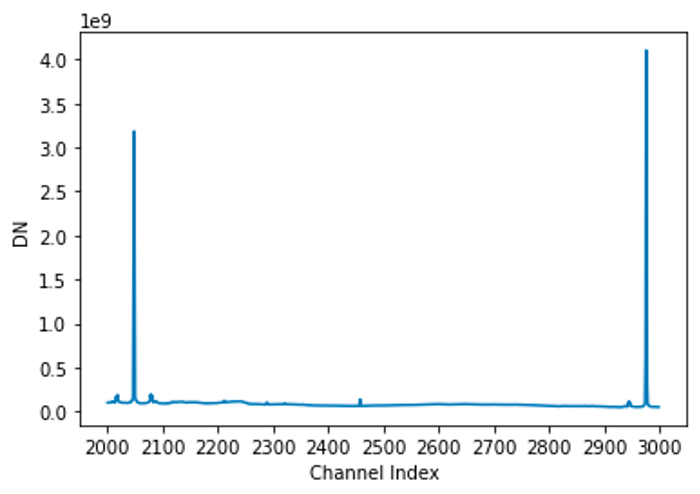
\includegraphics[width=0.49\linewidth]{figs/3/hasp1.png}
    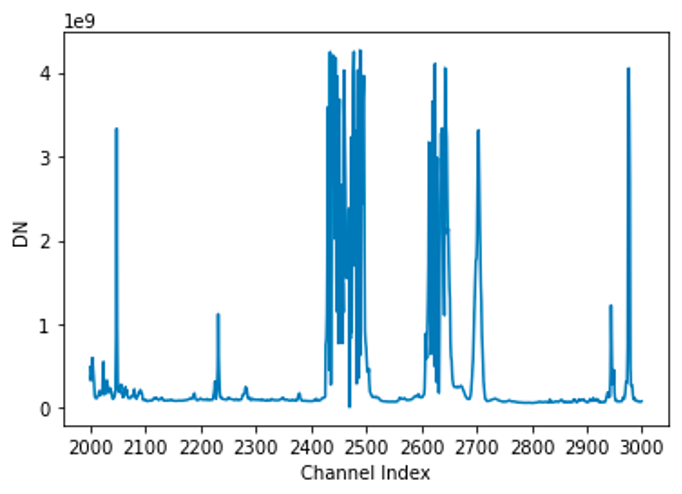
\includegraphics[width=0.49\linewidth]{figs/3/hasp2.png}
    \caption{Examples of spectra with the lowest (left) and highest (right) anomaly scores from the HASP dataset when using the PCA method to fit the entire HASP dataset.}
    \label{chap3/fig:hasp}
\end{figure}

One limitation of this dataset is that there aren't examples of changes in the baseline shape or bias readout level. 
These changes are rare and typically caused by physical changes in the instrument's hardware. 
In order to account for these, we would need to inject simulated anomalies in the data.
This is outside the scope of this work but will be discussed in Section \ref{chap3/sec:future}.

\section{Results and Conclusions}
\label{chap3/sec:results}
\begin{figure}[b]
    \centering
    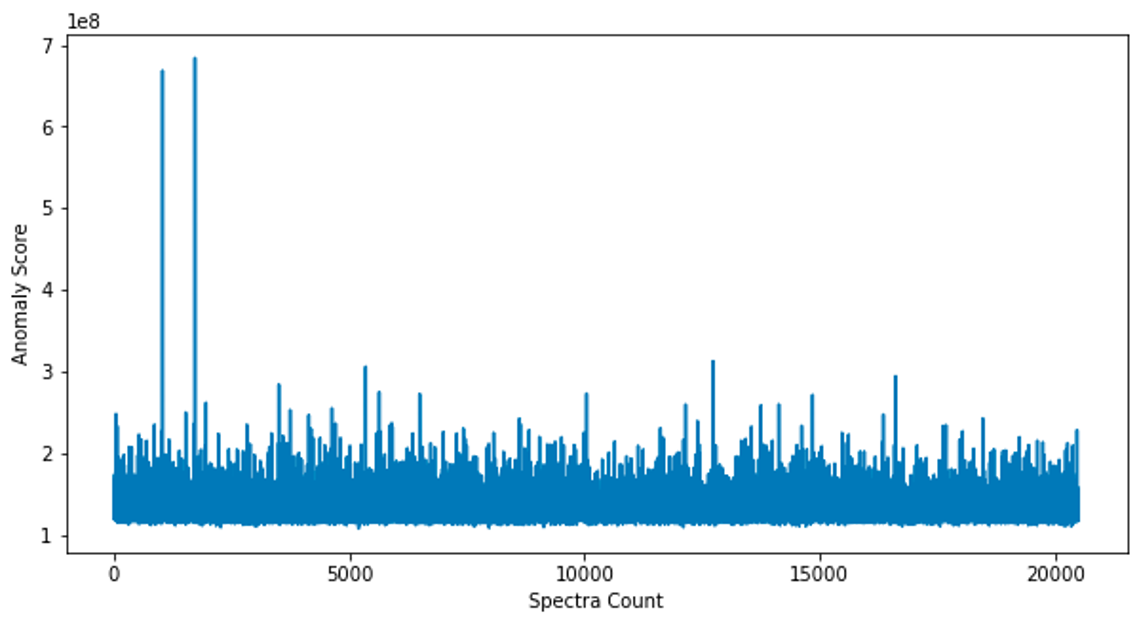
\includegraphics[width=0.5\linewidth]{figs/3/asthros_timeseries.png}
    \caption{A time series of anomaly scores using the PCA method for the 100GHz integration test data. Two large spikes are visible in the data indicating large changes between a spectrum and the previous spectra in the rolling window.}
    \label{chap3/fig:timeseries}
\end{figure}

Both datasets are unlabeled, which makes measuring accuracy difficult so we have to use more qualitative methods to compare the two.
The end use case of this is to provide a trackable metric that the operations team can use to monitor data quality.
While accuracy is certainly important, any method that is able to enhance the manual monitoring process is sufficient. 
As such, we compare the methods based on their ability to be implemented into the ASTHROS System Architecture and how well the anomaly score metric tracks with manual monitoring of the time series of spectra over time. 
Additionally, we can compare the least and most anomalous spectra form the system to what sorts of anomalies produce high anomaly scores. 

With both datasets, the large number of features in the $8192$ channels, made it difficult for the VAE to learn the latent space for the spectra. 
Even after we managed to get it to behave properly, it became apparent that this method wouldn't adapt well for a rolling window of previous spectra. 
We would have to retrain the system on the fly to ensure that it adapted to gradual changes in instrument behavior.
With more refining and tests with domain adaptation, we may be able to revisit this method but, due to the overhead of having to retrain and the overall complexity of the system, we opted to focus on more adaptable methods. 


PCA was an ideal method for this use case. 
We began with the HASP dataset to see how the method would be able to rank spectra from least to most anomalous.
We first fit all of the $7000$ spectra with PCA to determine the number of components that would be optimal for comparison.
Most of the variances was captured with the first two principal components but, we opted to use five components as the variance increases when we're only looking at a portion of the dataset as shown in Figure \ref{chap3/fig:elbows}.
Using these number of components, we calculate the anomaly score for all of the spectra in the dataset to review the least and most anomalous spectra. 
See Figure \ref{chap3/fig:hasp} for the least and most anomalous spectra in the dataset. 
We've zoomed into a range of indices that were heavily affected by RFI, likely from another instrument. 
As expected, the least anomalous spectra look relatively clean and the most anomalous spectra are all very noisy. 

\begin{figure}[t]
    \centering
    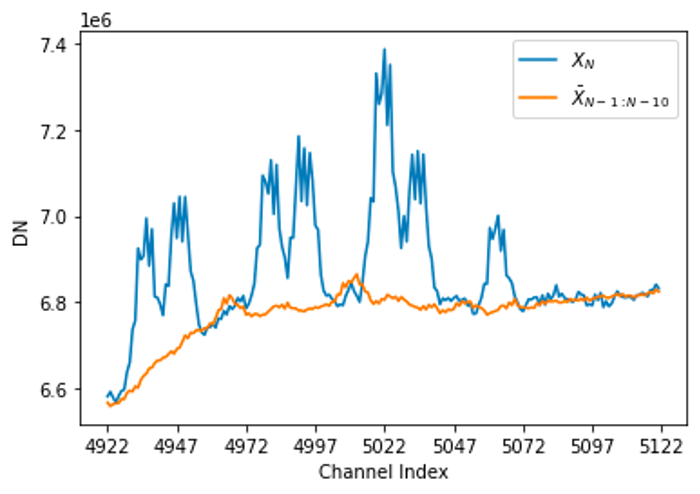
\includegraphics[width=0.49\linewidth]{figs/3/pca1.png}
    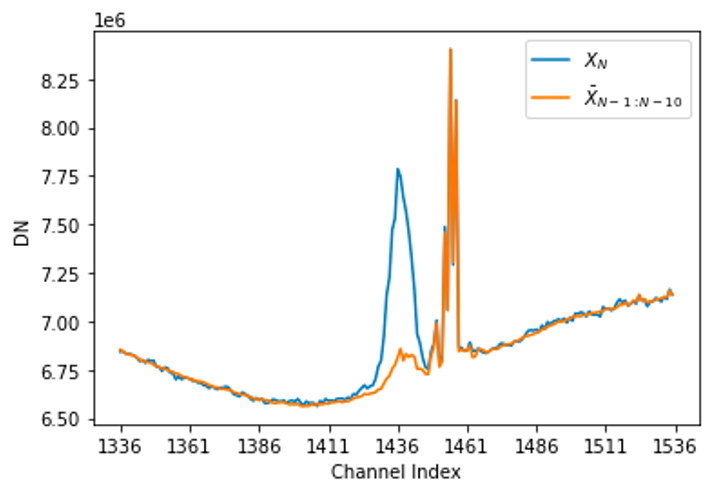
\includegraphics[width=0.49\linewidth]{figs/3/pca2.png}
    \caption{Examples from the 100GHz integration test data showing the spectra at the time of the two spikes in Figure \ref{chap3/fig:timeseries}. The blue line shows the spectra that has the high anomaly score and the orange line shows the average spectrum from the past 10 spectra. These spectra were highlighted due to the PCA method's inability to recreate the features shown in the new spectra when trained on the rolling window of previous spectra.}
    \label{chap3/fig:100ghz}
\end{figure}

On the cleaner 100GHz dataset, the method truly shined.
Using the same rolling window of 10 spectra and 5 principal components, we were able to produce a time series of anomaly scores for all 20,000 spectra as shown in Figure \ref{chap3/fig:timeseries}.
These values on their own don't provide much information but, when compared with other values across the dataset, we are able to pick out instances where our anomaly scores spiked. 
In the time series, there are two major spikes in the time series and a handful of smaller spikes throughout the test. 
We looked into these larger spikes in anomaly score and, they corresponded with spectrum that had changes in their RFI spikes.
Figure \ref{chap3/fig:100ghz} shows the affected channels of these anomalous spectra by overlapping them with the average of the previous 10 spectra. 
As shown in both examples, the new spectra has an increase in RFI that is different from the most recent spectra. 
On the other hand, the least anomalous spectra all closely match their predecessors. 
Of the tested methods, PCA has shown the most promise for implementation into the ASTHROS Readout System. 

\section{Future Work}
\label{chap3/sec:future}
The PCA method tested in this paper is currently being implemented onto the ASTHROS Readout Systems to test it in operations during ASTHROS's flight in 2024. 
The method will run on the analysis computer and integrate with the rest of the ASTHROS network to provide real-time data quality status messages over the RMQ status exchange.
During integration testing, the PCA method will be tested to ensure that it can handle the data rates and data sizes that will be produced during the flight. 

While the VAE method was less suitable for our use case, with more fine-tuning and optimization for the rolling window of past spectra, it could be a viable method for detecting anomalies in the future.
There are other methods, such as a Gaussian Mixture Model (GMM) or a Hidden Markov Model (HMM), that could be tested in the future to see if they are more suitable for our use case as well.

A limitation of our datasets are the lack of changes in shape of the spectrum or changes in bias level. 
In the future, we will make a simulator to inject these anomalies into our datasets to further test these methods. 
Additionally, with the flight of ASTHROS, we will have real calibration data to test everything on and reassess how we can improve our methods after using them for operations.
\chapter[Electron Density Mapping in Carina Nebula]{Electron Density Mapping in Carina Nebula}
\label{ch:carina}

To map electron density in Carina we begin with the following equation from \cite{pineda2018}.
\begin{equation}
    R^{[NII]}_{RRL} = 2.68 \times 10 ^ {-9} \nu_{RRL} T_e^{3/2} \frac{f(^3\text{P}_1)}{n_e} G^{-1}_{NLTE}(n_e,T_c)X_N
    \label{eq:ratio}
\end{equation}
In this equation we have the following variables:
\begin{itemize}
    \item $R^{[NII]}_{RRL}$: The ratio of the intensity of NII to the intensity of the Hydrogen Radio Recombination Line (RRL).
    \item $\nu_{RRL}$: The frequency of the RRL in Hz.
    \item $T_e$: The electron temperature in Kelvin.
    \item $f(^3\text{P}_1)$: The fractional population of the $^3\text{P}_1$ level of ionized nitrogen. 
    \item $n_e$: The electron density in cm$^{-3}$.
    \item $G_{NLTE}(n_e,T_c)$: The deviation from local thermodynamical equilibrium (LTE) for the hydrogen RRL emission.
    \item $X_N$: The abundance of nitrogen with respect to hydrogen.
\end{itemize}

Both $T_e$ and $X_N$ can be estimated using the distance to the Galactic center $R_{gal}$ in kiloparsecs (kpc). 
\begin{align}
    T_e &= (4446 \pm 301) + (467 \pm 34) R_{gal} \\
    12 + log(X_N) &= (8.21 \pm 0.09) - (0.059 \pm 0.009) R_{gal}
\end{align}

To solve for $n_e$ we can isolate the terms that rely on $n_e$ in Equation (5.1).
\begin{equation}
    \frac{f(^3\text{P}_1)}{n_e G_{NLTE}(n_e,T_c)} = \frac{R^{[NII]}_{RRL}}{2.68 \times 10 ^ {-9} \nu_{RRL} T_e^{3/2} X_N}
\end{equation}

The left side of Equation 5.3 has all the terms that depend on $n_e$ and the right side are calculated constants and the ratio of the intensities of the [NII] and RRL lines.
In \cite{pineda2018}, the authors provide a relationship between $n_e$ and the terms on the left side of the equation for various continuum brightness temperatures ($T_c$ or $T_b$).
In order to use this curve, I used the data provided in the paper to calculate the right side of the equation and fit the calculated values along with the reported $n_e$ values to a sigmoid.

\begin{figure}[h]
    \centering
    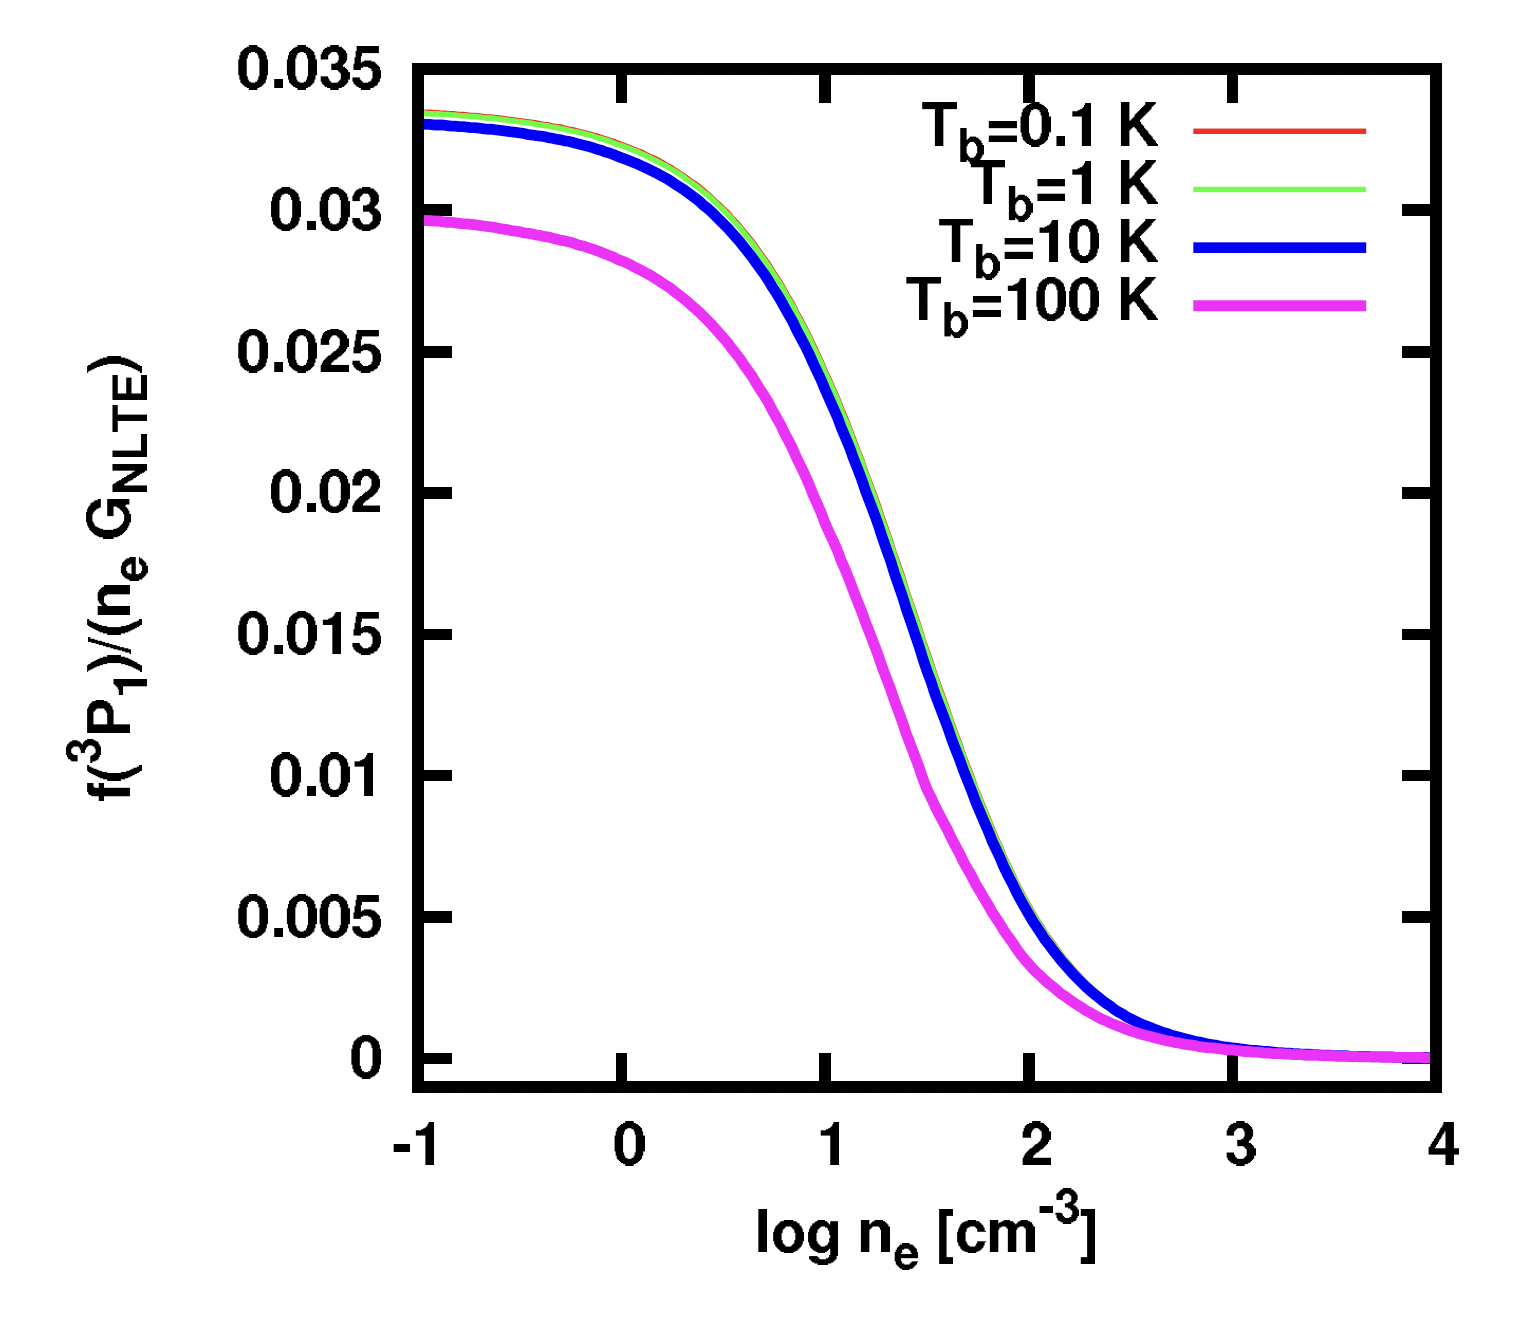
\includegraphics[width=0.4\textwidth]{figs/4/curve.png}
    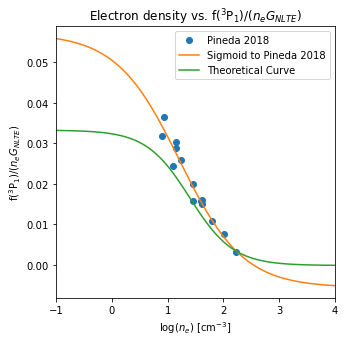
\includegraphics[width=0.4\textwidth]{figs/4/calculated_curve.png}
    \caption{The dependence of the [NII] 205 $\mu$m ratio on delectron density for a set of continuum brightness temperatures \cite{pineda2018}.}
    \label{fig:ne_vs_tc}
\end{figure}

With this sigmoid, we can now calculate the electron density for the Carina Nebula assuming our continuum brightness is between 0.1 and 10 K.
To prepare both spectral cubes we spectrally and spatially reproject the [NII] 205 $\mu$m and the Hydrogen RRL data to the same grid.
We then convolve the [NII] 205 $\mu$m data with the beam of the RRL data. 
Finally, we calculate the integrated intensities of both lines for the following locations.

\begin{table}[h!]
    \centering
    \begin{tabular}{|c|c|c|}
        \hline
        Location & $v_{min}$ km/s & $v_{max}$ km/s \\
        \hline
        Keyhole Nebula & -40 & -20 \\
        Carina Extended & -20 & 20 \\
        \hline
    \end{tabular}
    \caption{The spectral slabs of Carina Nebula used to calculate the electron density.}
    \label{tab:carina}
\end{table}

The resultant electron density map is shown in Figure \ref{fig:ne_map_keyhole} and \ref{fig:ne_map_carina}.

\begin{figure}[h]
    \centering
    
\includegraphics[width=\textwidth]{figs/4/ne_map_keyhole.png}
    \caption{The electron density map of the Keyhole Nebula.}
    \label{fig:ne_map_keyhole}
\end{figure}

\begin{figure}[h]
    \centering
    
\includegraphics[width=\textwidth]{figs/4/ne_map_carina.png}
    \caption{The electron density map of Carina Extended.}
    \label{fig:ne_map_carina}
\end{figure}


\chapter[Anomaly Detection for the Roman Space Telescope Wide Field Instrument’s Science Data Processing Pipeline]{Anomaly Detection for the Roman Space Telescope Wide Field Instrument’s Science Data Processing Pipeline}

\section{Abstract}
The Roman Space Telescope (RST) Wide Field Instrument (WFI) will be utilizing a preliminary Science Data Processing (SDP) pipeline during its Integration and Test, and to some extent during Operations, to track basic statistics and identify known features such as cosmic rays, snowballs as well as possible anomalies in raw detector data. 
In our detectors, these anomalies appear as jumps in the ramp of a readout and are classified as cosmic rays if they appear as a streak or snowballs if they're more circular. 
The WFI employs an array of 18 H4RG-10 detectors that collect image samples.
Each set of raw frames within a non-destructive exposure is packaged by the SDP pipeline into image cubes for each detector.
Each cube is a time series of $4096 \times 4096$ accumulating pixel frames.
The preliminary analysis pipeline is used to locate anomalies in these time-series accumulation frames and identify the type of anomaly, either natural phenomena or detector characteristic.
To compare different methods, we've implemented both heuristic-based and data-driven methods to identify anomalies.
For the heuristic-based approach, we identify snowballs and cosmic rays by the size and shape of outlier pixel clusters between consecutive frames.
For data driven methods, we evaluated a Convolutional Neural Network (CNN) model, and more traditional methods like Principal Component Analysis (PCA).
CNN is a supervised learning/classification method. 
Thus, we used a labeled dataset of anomalies to perform segmentation of the image and identify anomalies. 
We used previously identified cosmic rays and snowballs to measure the accuracy and efficiency of the mentioned approaches. 
In evaluating these methods, we aim to pick the best fit for the SDP pipeline's anomaly detection in terms of both performance and runtime. 

\section{Introduction}
The Roman Space Telescope (RST) Wide Field Instrument (WFI) employs an array of 18 H4RG-10 detectors to collect image samples.
Each detector on the WFI utilizes a up-the-ramp readout scheme that produces $4096 \times 4096$ pixel images at each frame along the exposure. 
For a given exposure, each frame gives us information on the amount of light collected over time and allows us to identify both the location and time of anomalies within a ramp.
During an exposure, natural or detector-related events may occur that affect groups (or sets) of pixels across the detector. 
Because we're collecting time-series information, we can see the exact frame that the event occurs and observe how the event affects subsequent frames. 
There are many different sources that might cause errors in our detectors' data, such as read noise patterns, thermal noise, compression errors, and software errors, but in this paper, we are particularly interested in external and natural sources of errors \cite{cillis2018snowballs}. 
Both cosmic rays and snowballs are transient events that result in sudden increases in charges and pixels’ Data Number (DN) values, compared to their typical neighboring pixels.
These events are also rare.
Therefore, we can use anomaly detection to identity these outliers.
Figure \ref{chap5/fig:anomalies} shows examples of these two events.

\begin{figure}[h]
    \centering
    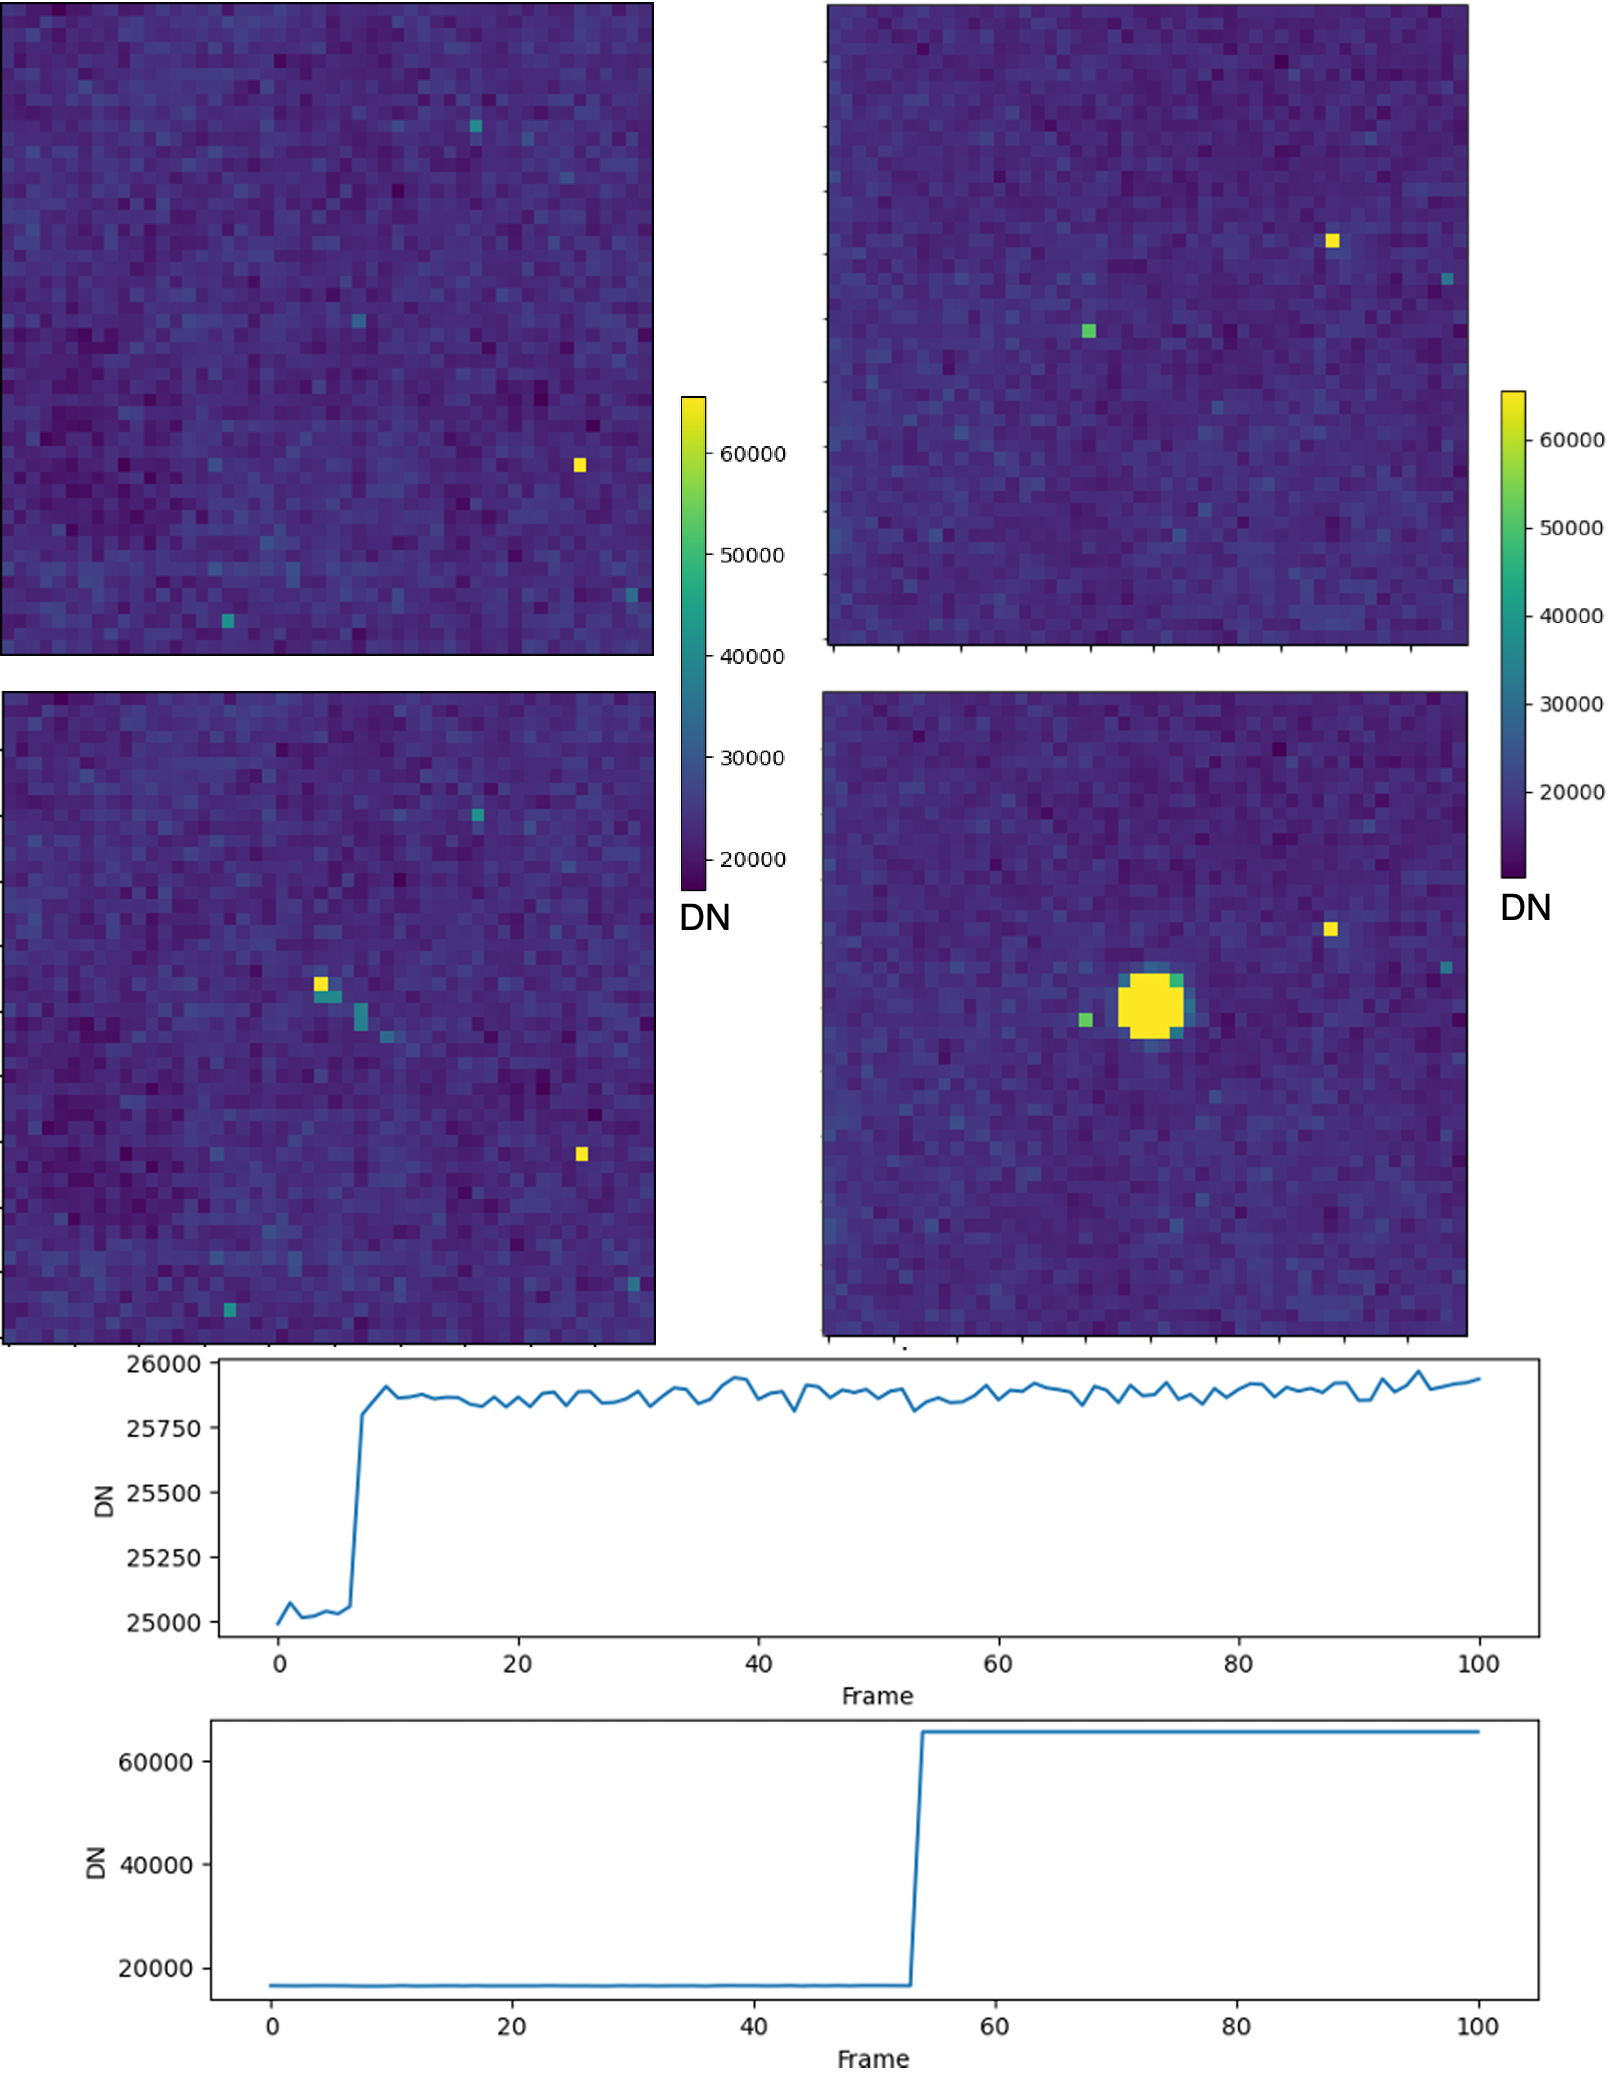
\includegraphics[width=.75\linewidth]{figs/5/Examples_fixed.png}
    \caption{An example of a cosmic ray (left) and snowball (right) in RST's detector data. The top frames show the frame prior to the event and the bottom frames show the area after the event occurred. The bottom graphs show the overall DN value across the entirety of the exposure, showing large jumps at the time of the event for the cosmic ray (top) and snowball (bottom).}
    \label{chap5/fig:anomalies}
\end{figure}

An anomaly is defined as an unexpected occurrence in a sequence based on a data set of typical sequences \cite{horton2021integrating}. 
Given our image is mostly typical pixels, we can use this feature to identify out of distribution pixels that may be caused by snowballs or cosmic rays. 
While snowballs are a relatively newly recognized detector phenomenon, detection and rejection of snowballs are common practices for astronomical images \cite{van2001cosmic}.
These cosmic rays appear as streaks across multiple pixels within an exposure as the incident cosmic ray imparts energy as a point spread function across neighboring pixels \cite{pych2003fast}.

Both snowballs and cosmic rays will appear as jumps in DN value in a ramp but the shape of the affected neighboring pixels helps us differentiate between the two.
Snowballs will be circular in shape and affect 8 or more pixels \cite{cillis2018snowballs}.
On the other hand, Cosmic Rays will be any grouping larger than 2 pixels that shows a linear streak. 

The goal of our anomaly detection is to highlight these features as part of the RST WFI SDP's pipeline. 
As such, SDP's processing time should keep up with data generation time so that we can identify issues within the detectors as we collect new data. 
This poses a challenge due to the massive data size of the data products from the array of 18 detectors. 
To address this challenge, raw data is automatically processed into interpretable products as part of the SDP pipeline. 
As this anomaly detection system will be part of the SDP pipeline as an additional data product, the runtime of any method must be taken into account along with the method's accuracy. 

The rest of this paper is organized as follows.
First we go over the methods for identifying and classifying snowballs and cosmic rays in Section \ref{chap5/sec:methods}.
Then, in Section \ref{chap5/sec:data} we explain the dataset chosen and how labels for the dataset were generated.
After that, we discuss the results of the different methods and draw conclusions about which methods to implement in the SDP pipeline in Section \ref{chap5/sec:results}.
Finally, we go over future works in Section \ref{chap5/sec:future}.

\section{Methods}
\label{chap5/sec:methods}
To identify the anomalies in our data, we split our problem into two distinct tasks: 1) locating and grouping pixels that have irregular ramps and 2) classifying those pixels as cosmic rays, snowballs, or something else entirely.
By splitting our anomaly detection into two tasks, we can use the first step to identify regions of interest and reduce our search area for snowballs and cosmic rays to that of anomalous pixels.
This can drastically reduce the amount of pixels we have to classify as we also identify the frame that the anomaly occurred in, reducing our focus to a smaller window around the event. 
The following are potential candidate methods for accomplishing these two tasks.

\begin{table}[h]
    \centering
    \begin{tabular}{l|l}
        \textbf{Step 1: Locating Anomalies} & \textbf{Step 2: Classifying Anomalies} \\
        Statistical Thresholding & Heuristic Rules\cite{cillis2018snowballs} \\
        Principal Component Analysis (PCA)\cite{wold1987principal} & Convolutional Neural Network (CNN)\cite{gu2018recent}
    \end{tabular}
    \label{chap5/tab:methods}
\end{table}

There are other viable methods for accomplishing these tasks, such as Reed-Xiaoli (RX), Localized Reed-Xiaoli (LRX), and James Webb Space Telescope's (JWST) Bayesian Generalized Least Squares (GLS) for locating anomalies, but the scope of this work will focus on the methods in Table \ref{chap5/tab:methods}.
RX is an unsupervised learning methods that uses a window around a test pixel to compare with the local background \cite{reed1990adaptive}.
LRX is similar to RX but instead uses a double concentric window to compare the test pixel with a guarded local background \cite{molero2013analysis}.
JWST's GLS estimator is also an unsupervised method that calculates the slope, or ramp, of each pixel along the time domain and determines the probability that discontinuities in the ramp occurred due to cosmic rays \cite{robberto2015cr}.
Please note that the JWST data was constructed similarly to the RST's, resulting in non-destructive accumulating frames. 

Before any of the data is used for these methods, they must be loaded and pre-processed.
For more information about this and the dataset selection, see Section \ref{chap5/sec:data}.

\subsection{Locating Anomalies}
\begin{figure}[b]
    \centering
    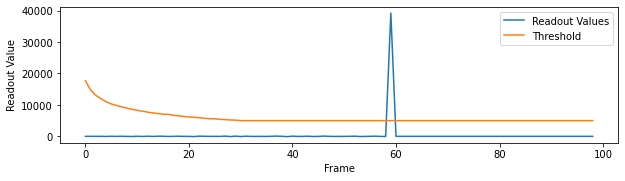
\includegraphics[width=1\linewidth]{figs/5/Threshold.png}
    \caption{The readout values for a flagged pixel. The read out values are the amount of DN gained in a given frame. We compare this value to our calculated threshold and, if surpassed, that specific location and frame is flagged for classification.}
    \label{chap5/fig:threshold}
\end{figure}
To locate the anomalies, we looked for methods that would be able to not only identify where a potential anomaly is located but when the event occurred that caused the anomaly. 
\subsubsection{Statistical Thresholding}
Our initial approach is readout thresholding, where we take two subsequent frames, $x_i$ and $x_{(i-1)}$ where $n$ is the number of frames in an exposure. 
For each readout frame $\Delta x_i$, we calculate the mean $\mu_i$ and standard deviation $\sigma_i$ across its pixels. 
We use these values to calculate the threshold for jumps in the ramp with a minimum threshold value of 5000 DNs.
\begin{equation}
    \Delta x_i > \max(\mu_i + 50 \sigma_i, 5000)
\end{equation}
These values were chosen for dark frames as they allow us to easily identify large jumps traditionally associated with snowballs or cosmic rays. 
From here, we create a pixel mask for each frame of all readout values that exceed this threshold. 
We then preform a series topological transformations to bridge and fill in incomplete holes through dilation, binary hole fill, and erosion procedures using SciPy's ndimage library \cite{2020SciPy-NMeth}.
Finally, we remove any grouping of pixels of two pixels or less to ensure any jumps in the ramp we discover affect multiple pixels and then use scikit-image's measure library to locate the central pixel for each group \cite{scikit-image}.
We are then left  with groupings of pixels that could potentially be either a cosmic ray or snowball.


\subsubsection{Principal Component Analysis (PCA)}
Given the majority of pixels within our image aren not affected by anomalies, we can use a random subset of pixels within an exposure and fit PCA to the ramps of these samples.
If we limit our principal components to two, we can create a fit for the majority of simple ramps. 
Using our PCA fit, we can reduce all of the pixels in our image to our latent space representation and then inverse transform them to compare the original and reconstructed result \cite{wold1987principal}
Examples of this are shown in Figure \ref{chap5/fig:PCA}. 
\begin{figure}
    \centering
    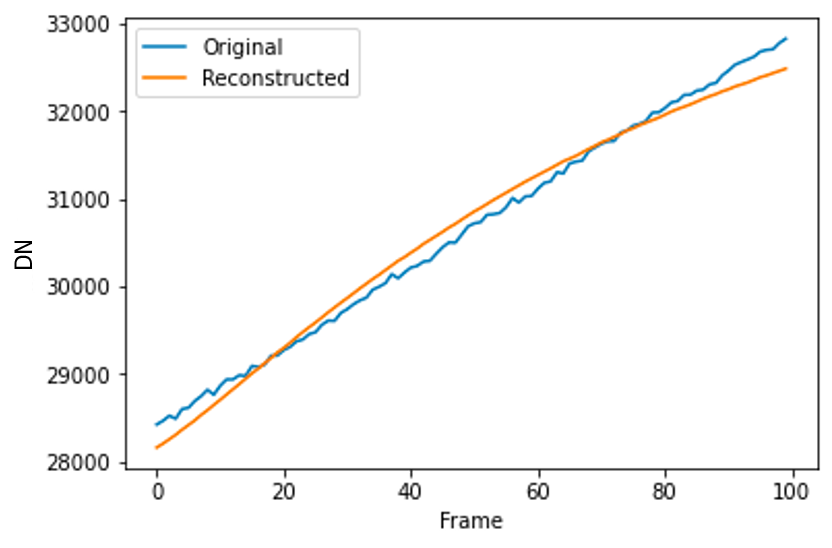
\includegraphics[width=0.49\linewidth]{figs/5/PCA_Good.png}
    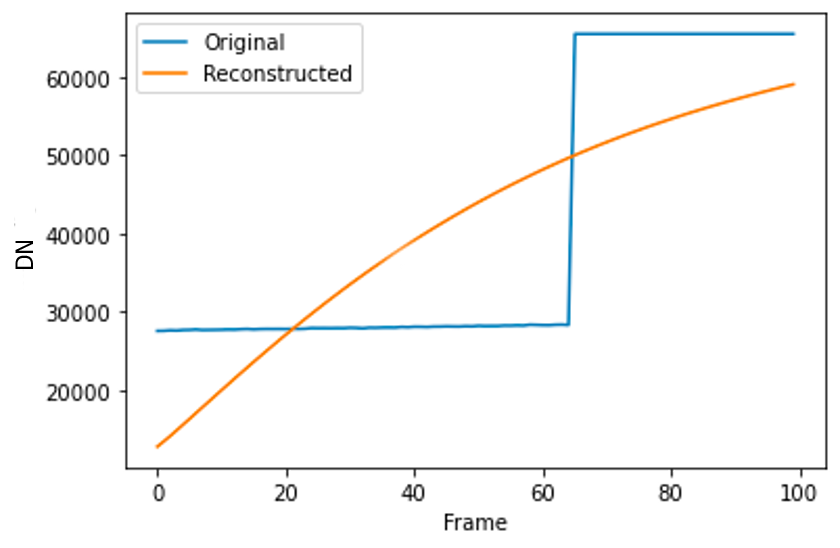
\includegraphics[width=0.49\linewidth]{figs/5/PCA_Bad.png}
    \caption{Examples of reconstruction of ramps using PCA. The DN values for the reconstructed image are calculated by transforming the original values and then inverse transforming our original ramp using only a subset of the principal components (i.e. two) to reproduce the shape. By limiting the number of principal components to two, we can have the reconstructed image fit the shape fairly well for normal ramps and not fit ramps with anomalies.}
    \label{chap5/fig:PCA}
\end{figure}

With the reconstructed values, we are able to calculate the residual ($Image_{Reconstructed} - Image_{Original}$) of the errors and identify where anomalies occur based on spikes in the ramp of the residual. 
To identify these spikes, we can employ a similar method to the Statistical Threshold method to calculate the change in residuals between each frame and find out of distribution values. 
This results in identifying the frames for each pixel that have large jumps in the residual. 
By limiting the number of PCA components to two, our reconstructed ramps will be relatively smooth, causing original ramps that have large jumps in them to have a large change in residual at the frame of the event.

Finally, like the statistical method, we create the pixel mask by highlighting any pixel whose change in residual is above the threshold.
We then identify regions using the same topological transformations and scikit-image's measure library for finding blobs \cite{scikit-image}.

\subsection{Classifying Anomalies}
From the locating anomalies methods, we obtain a frame and pixel mask matrix containing information about potential anomalies with a ramp for each pixel in an exposure. 
We also obtain a table listing groupings of pixels to classify. We call this table the Event Table as it describes the time and location of potential anomalies. 
These groupings are the input into our classification methods as they help limit the search to specific pixels and frames across the exposure. 

\subsubsection{Heuristic Rules}
For heuristic rules, these groupings are labeled and measured by the number of pixels affected and the major and minor axes lengths of the affected area. 
We use these values to determine the type of anomaly.
Snowballs are large circular anomalies that cover 9 or more pixels.
Cosmic rays are oblong anomalies that cover more than 2 pixels. 
We determine the circularity of the anomaly be comparing the minor and major axis using the following criteria.
\begin{align*}
    \text{Circular:}\ &  \text{minor\_axis} \geq \text{major\_axis}/2 \\
    \text{Large:}\ & \text{area} \geq 9
\end{align*}

From this we are able to produce two output products: a new data cube where each frame is a mask identifying pixels affected by anomalies, and an updated Event Table with information about each anomaly. 

\subsubsection{Convolutional Neural Network}
\label{chap5/sec:CNN}
For each listing in the Event Table, we take a 32 square pixel sample region around the central pixel spatially and the three frames around the event frame for a sample of $32 \times 32  \times 3$ pixels. 
This is the input into our CNN which is trained using hand labeled data from the DCL dataset. 
The CNN architecture processes input images through two convolutional layers followed by ReLU activations and max pooling, which flattens the output.
Finally we pass the output through two fully connected layers to produce class scores for None, Cosmic Rays, Snowballs, and Potential Anomalies classes based on the labeled dataset.
We preformed two tests with the CNN by training and testing on our all of the labeled dataset and just the data from the same detector to see how well the method generalizes. 
Both tests were preformed with an 80/20 test/train split with balanced classes. 
The output classes from the CNN are then used to label the pixels in the mask with their associated class and update the Event Table with anomaly labels. 
\subsection{Output Products}
To align with the rest of the products from the SDP pipeline, we package the outputs from the anomaly detection pipeline as Hierarchical Data Format 5 (HDF5) files \cite{The_HDF_Group_Hierarchical_Data_Format}.
HDF5 is a file format that is designed to store large amounts of data and is perfect for the types of products we need to produce for the SDP.
Because of HDF5's efficient read/write procedures, the SDP is able to keep up with the data generation rate while producing analysis products. 
For each exposure, we produce three binary mask arrays for events labeled as Cosmic Rays, Snowballs, and Potential Anomalies for each pixel within a ramp. 
These binary masks are the same shape as the exposure and allow us to quickly identify and flag problem pixel/frame combinations in an exposure. 
We also produce a single image for each anomaly type where each pixel is the frame number of an event. 
This allows us to visualize anomalies and see how they may change throughout an exposure.
Finally, the Event Table is formatted so that each row in the HDF5 array is an anomaly that has central pixel, size, shape (semi-major and semi-minor axis), and classification as columns. 
These products are produced during SDP pipeline and added as part of the automated report. 
\section{Data}
\label{chap5/sec:data}
The H4RG detectors used in the WFI array are able to perform non-destructive reads while producing an exposure resulting in measurements through time, also referred to as up-the-ramp measurements. 
This allows us to take the up-the-ramp measurements taken during an exposure and order them in a series to create frames within the exposure. 
This results in a time series of frames for each integration from a detector's pixel values being reset at the beginning of an exposure to the final accumulated pixel values at the end of an exposure \cite{jwstjdoc} \cite{casertano2022determining}.
For testing the effectiveness of the anomaly detection pipeline, we will be utilizing real exposures taken during the selection phase of the flight detectors for the WFI detector array. 
During the selection phase of flight detectors, over 70 detectors went through numerous experiments with different types of light exposures, both bright and dark.
The dark tests consisted of a two-hour long exposure where detectors accumulated across 100 frames.
These tests are ideal to identify cosmic rays and snowballs due to their long exposure time, resulting in more opportunities for anomalies to appear in the frames. 
For the purposes of testing these methods, this paper focuses on using just these dark exposures. 

The data from these tests are provided in the form of Flexible Image Transport System (FITS) files that consist of 101 frames of $4096 \times 4096$ pixel images \cite{wells1979fits}.
The first frame in an exposure is the reset frame and can be disregarded. 
The FITS data is loaded into a NumPy array of unsigned integers by iterating over the array \cite{harris2020array}.
To correct the read direction of FITS data, the data is processed by subtracting every pixel values from the maximum possible DN value for each pixel, $2^{16} - 1$, across all frames.
This leaves us with a data cube of $100$ frames, each with $4096 \times 4096$ pixels. 

The data provided by the DCL lab contains labeled information about known snowballs during the exposure. 
These snowballs are our preliminary ground truth for identifying the effectiveness of our methods. 
In addition to these snowballs, the outputs for each method are reviewed to identify snowballs and cosmic rays that are not in the original labels
Because the heuristic method is overly sensitive, each anomaly highlighted by the method was hand labeled as potential anomaly, cosmic ray, snowball, or non-anomaly. 
These hand labels are used to measure the accuracy of each method and train methods such as the CNN in Section \ref{chap5/sec:CNN}.

\section{Results and Conclusions}
\label{chap5/sec:results}

As we are able to split our system into two different subsystems, the results here will discuss which of the methods are best for accomplishing each individual task. 
Then we will go more in depth with the best pairing of methods integration into the RST WFI SDP. 
For consistency all of the tests were preformed on a 2021 M1 Macbook Pro Max with 64GB of unified memory.
Much of the development of this work was done on NASA Center for Climate Simulation PRISM GPU cluster. 

\subsection{Locating Anomalies}
The two methods we tested for locating anomalies were statistical thresholding and PCA.
Both methods look for large jumps in a time series but each method is looking for a different type of jump.
The statistical thresholding method is purely looking for jumps in the DN accumulated each frame by identifying large changes in DN compared to the rest of the accumulated DN in the frame. 
The PCA method trains on a subset of pixels across the exposure and is looking for large jumps in the residual error from transforming and inverse transforming each pixel. 
For performance, both methods require calculating the difference between values, a threshold, and then identifying groups of flagged pixels. 
On average, this takes about 2 minutes and 10 seconds for each dark image with 100 frames. 
Because the PCA methods needs to fit, transform, and inverse transform the entire exposure, running it adds on an average of 42 seconds to locating anomalies. 
This makes the Statistical Threshold method faster than PCA in every experiment due to PCA requiring pre-processing. 

\begin{figure}
    \centering
    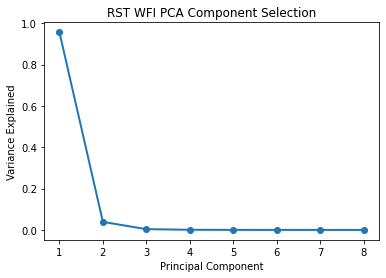
\includegraphics[width=.5\linewidth]{figs/5/elbow.png}
    \caption{Elbow plot for the PCA method on typical ramps. A limit of 2 components was selected to ensure we aren't over fitting to the curve and missing anomalies.}
    \label{chap5/fig:elbow}
\end{figure}

As for performance, both methods are over-sensitive to false positives.
The PCA method found less groupings than the statistical thresholding method but many of the omitted locations are false negatives.
We chose to use two principal components as any higher numbers of components would have fit to jumps in the ramp and caused lower errors.
Two components also gives us an overall shape that matches a typical ramp and explains most of the variance of the exposure's ramps without over fitting to the curve as shown in in Figure \label{chap5/fig:elbow}.
This false negative rate varies from exposure to exposure but ranged from 65 to 80\% missed anomalies. 
Despite being overly sensitive to any jump in the ramp, the statistical thresholding method is preferred here due to it's higher accuracy and lower runtime.
This method had a false negative rate of 10\% across the entire labeled dataset of over 5000 hand labeled events. 
A method that filters most of the image without removing real anomalies is preferable to a method that filters more of the images including anomalies. The second step, Classifying Anomalies, can then label these false positives as None or Potential Anomaly. 
\subsection{Classifying Anomalies}
For classifying anomalies, we have the traditional method using heuristic rules around the shape of the grouping and a CNN trained on samples from the labeled anomalies. 
We utilized the output of the statistical thresholding method as the input into both of the classification methods. 
Neither method were spectacular at accomplishing the task but the heuristic rules method did outperform the CNN by a wide margin. 

We experimented with the CNN by training it on a subset of events in the Events Table that were hand labeled by humans and then testing it on a separate set of events. 
We tested training using a subset of all exposures in the labeled dataset as well as just exposures from a specific detector.
In both cases, we were unable to have the CNN generalize to different exposures. 
Because of the class imbalance and hard to differentiate nature of the dataset, the CNN would misclassify cosmic rays as potential anomalies and almost never correctly identify them as cosmic rays unless the streak was large enough to differentiate. 
The CNN was able to correctly classify snowballs about 50\% of the time, labeling them as potential anomalies in other cases. 
In the future, this method may be better suited than heuristic rules but further refining of the labeled dataset is necessary. 
As it stands, with the overlap between cosmic rays and potential anomalies, there is little room for improvement without further defining how we want to differentiate these classes. 

Heuristic rules outperformed our CNN method in both accuracy and runtime.
The outputs from Event Table in locating anomalies include measurements of the size and shape of the anomaly. 
This makes it very efficient to run through each entry of the table and pre-define a look up table to classify each anomaly. 
The time the heuristic rules pipeline takes to generate a report depends on the number of anomalies in the Event Table but, on average, it is able to classify 100 events from the Event Table a second. 

\subsection{SDP Pipeline Integration}
Of the methods tested, the best combination of methods for the SDP pipeline would be the Statistical Thresholding method for locating anomalies and the Heuristic Rules method for classifying anomalies.
This combination method was able to find every pre-labeled snowball from the original dataset and correctly identify 85 out of 137 (62\%) of hand labeled snowballs. 
The method also over classified cosmic rays by identifying many potential anomalies and non-anomalies as cosmic rays.
This is likely due to the less rigid criteria for identifying cosmic rays compared to snowballs.
Figure \ref{chap5/fig:heuristic_confusion} shows the confusion matrix for the Heuristic Rules method with the located data from the Statistical Thresholding method.
This method is currently being used in the SDP pipeline to identify anomalies in the WFI detector data.
\begin{figure}[h]
    \centering
    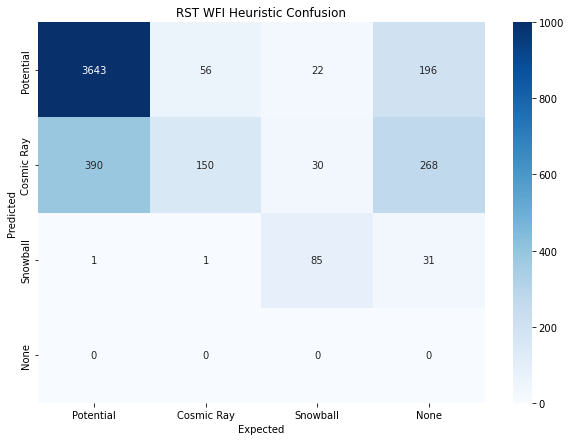
\includegraphics[width=.7\textwidth]{figs/5/heuristic_confusion.png}
    \caption{Confusion Matrix for the Heuristic Rules Method with Located Data from Statistical Thresholding.}
    \label{chap5/fig:heuristic_confusion}
\end{figure}

\section{Future Work}
\label{chap5/sec:future}
This work is a preliminary analysis of the anomaly detection methods for the RST WFI SDP pipeline.
There are many areas for improvement and future work to be done.
First and foremost, more methods will need to be evaluated in order to determine a better alternative to the Heuristic Rules method for classification. 
The CNN method is a good candidate but needs more fine tuning to generalize to different exposures.
In addition to this, more labeled data will be needed to train the CNN and other methods, such as Mask RCNN or transformer-based architectures, particularly on illuminated data.
This labeled data could come from other tests if we were to generalize beyond just the dark exposures.
With a more well defined dataset of labeled data, we will be able to better assess the accuracy of these methods too. 

Another area for improvement may be finding better ways to locate anomalies.
We may revisit PCA to see if we can adjust the parameters (number of components and threshold for error) to see if we can have it not discard real anomalies. 
Additionally, other methods like RX, LRX and GLS, as described at the beginning of Section \ref{chap5/sec:methods}, could be better suited for filtering the initial exposure.

The current implementation of the SDP pipeline uses a bad pixel mask to mask regions of the image that are problematic. 
Because we didn't have a bad pixel mask for the data we were using, we had to analyze the entire image with our anomaly detection methods.
This led to a large number of false positives from known bad pixels that appeared as anomalies in the dataset due to their sharp ramp in DN values at the beginning of the exposure.
In the future, we will need to integrate the bad pixel mask into the anomaly detection pipeline to filter out these false positives and use that to better assess the accuracy of the system. 

Finally, we will need to test the system on more than just dark exposures.
The current system is designed to work with dark exposures but we will need to adjust the system to work with other types of exposures that might have more difficult to detect anomalies.
There may not be a one size fits all solution to this problem but testing different types of exposures will help us determine the best methods for each type of exposure.
%\chapter[ASATHROS Payload Readout System Design]{ASTHROS Payload Readout System Design}
ASTHROS, the Astrophysics Stratospheric Telescope for High Spectral Resolution Observations at Submillimeter-wavelengths, is a balloon-borne observatory designed to study the universe in the submillimeter wavelength range.
The readout system is responsible for controlling the detectors, reading out the data, and storing the data on a solid state drive.
The readout system is designed to be modular and scalable, allowing for easy integration of new detectors and readout systems.
Each module is designed to be self-contained, focusing on a single device in the readout system so that changes to the hardware can be made without affecting the rest of the system.



\section{PMCC}
For ASTHROS, we utilize an array of 4GHz spectrometers called the PMCC ASIC P19800B ASIC RF Spectrometer, henceforth referred to as the PMCC.
These PMCCs are interfaced with via SPI for control, diagnostics, and readout \cite{PMCCP19800B}.
To communicate with the PMCCs, we utilize Raspberry Pi Compute Module 4s (CM4s) with custom harnesses.
The CM4 was chosen because it can be configured to operate at the 1.8V logic level necessary for PMCC by moving a diode on the CM4 IO board \cite{cm4io}.
Additionally, the CM4 has 4 SPI buses, allowing us to control up to 4 PMCCs per device \cite{cm4}.
The PMCCs are also connected to a GPIO pin on the CM4 to allow us to send a reset signal to the PMCCs.
The custom harness used to connect the PMCCs to the CM4 mounts onto the CM4 IO board's GPIO pins and converts the 40 ribbon cable to four sets of connections for the PMCC's SPI and reset pins.
Additionally, the CM4 has an SSD mounted to the side of it's IO board enclosure for raw spectra storage and easier local debugging when the device is not connected to the rest of the readout network.
Finally, two CM4s and eight PMCCs are mounted in a custom enclosure that is designed to be mounted on the back of the ASTHROS primary mirror.

PyMCC is the Python module developed to interface with the PMCCs and communicate with the rest of the readout system.
Originally, the PMCCs were controlled by a C program that was designed to provide a simple CLI for manually controlling the PMCCs.
As we needed to control multiple PMCCs and have them communicate with the rest of the readout system, we decided to rewrite the control software and drivers in Python.
The core of PyMCC is a Python driver for the PMCCs that provides an interface for controlling the PMCCs and reading out the data.
Built on top of the driver are Python programs that allow for manual control of the PMCCs, as well as a server that allows for control of the PMCCs over the RabbitMQ network.

\subsection{SPI Utilities}
At the lowest level of the PyMCC driver is the \texttt{spi\_utils} module.
This module provides an interface for communicating with the PMCCs over SPI using the \texttt{spidev} Python library.
The \texttt{spidev} library provides an interface to the Linux kernel's SPI device driver \cite{spidev}.
Additionally, the PMCC has 16-bit registers that require us to send and receive 16-bit words instead of the typical 8-bit bytes that \texttt{spidev} expect. 
This was the primary reason for the development of the \texttt{spi\_utils} module as it handles the conversion between 16-bit words and 8-bit bytes and provides an easier interface for configuring the PMCCs registers without having to worry about the low-level details of the SPI communication.

The \texttt{spi\_utils} module provides a \texttt{PMCC\_SPI} class that is used to communicate with the PMCCs.
The \texttt{PMCC\_SPI} class is initialized with the bus, device, SPI mode, bits per word, and clock speed for the PMCC with which we are communicating.
The bus and device are specific to the PMCC we are communicating with and are based on the wiring harness used to connect the PMCC to the CM4.
The SPI mode, bits per word, and clock speed are all set to the values specified in the PMCC manual.

To simplify addresses, the \texttt{PMCC\_SPI} object has a \texttt{make\_addr()} method that takes the address of the register we want to write to and the read/write bit.
Valid addresses for the PMCC are 0-511, and the read/write bit is 0 for a write and 1 for a read.
When sending a command to the PMCC, the first word of the command is the address of the regster we want to write to shifted left by 1 bit to make room for the read/write bit.
\begin{equation}
    \text{tx[16]} = \text{addr[9]} << 1 + \text{rw[1]}
\end{equation}
Because \texttt{spidev} uses 8-bit communication, we need to split the 16-bit word into two 8-bit bytes.
\begin{equation}
    \label{eq:split_word}
    \text{byte[8][2]} = [\text{word[16]} >> 8,\ \text{word[16]}\ \text{\&}\ \text{0xFF}]
\end{equation}
The helper method returns these two bytes as an array that can be used in other methods to convert an address and command into a format that can be sent over SPI.

For reading and writing to the PMCC, the \texttt{PMCC\_SPI} object has an \texttt{xfer()} method that takes the address of the register, a read or write flag, and optional data to write and length of data to read.
By default, the length of data to read is 1, and the data to write is None.
The \texttt{xfer()} method first obtains the TX bytes from the \texttt{make\_addr()} method.
For both read and write commands, we utilize the \texttt{spidev} library's \texttt{xfer3()} function as it allows us to send and receive data of arbitrary length in a single SPI transaction \cite{spidev}.
\texttt{spidev}'s \texttt{xfer2()} and \texttt{xfer()} will fail at list values longer than the maximum SPI buffer size.
On the other hand, \texttt{xfer3()} will automatically split the data into multiple SPI transactions if the data is longer than the maximum SPI buffer size.
This is vital for burst reads on the PMCC as our data can be much longer than the maximum SPI buffer size.
For writes, the \texttt{xfer()} method sends the TX bytes and the data to write to the PMCC.
The data is split into two 8-bit bytes using Equation \ref{eq:split_word}.
During this transaction, the PMCC does not send any data back, so the \texttt{xfer3()} function returns an array of zeros.
If our transaction is unsuccessful, instead of returning zeroes, we will receive an empty array that we can check for.
For single register reads, the \texttt{xfer()} method sends the TX bytes followed by a dummy word to the PMCC.
While we are sending the dummy word over the MOSI line, the PMCC is sending the data we requested over the MISO line that is returned by the \texttt{xfer3()} function along with the original TX bytes.
After checking that we have received data from the PMCC, we return the data as an array of 16-bit words.
This is done by utilizing NumPy to cast the output as a \texttt{np.uint8} array and then returning a view of that array with big-endian 16-bit unsigned integer data type.
For reads that are longer than a single register, we send the TX bytes followed by a dummy word for each word we want to read and follow the same process as a single register read.

For simple reads, \texttt{PMCC\_SPI} has a \texttt{read()} method that takes the address of the register we want to read from and optionally the number of words we want to read.
By default, this method reads a single word from the PMCC.
The \texttt{read()} method calls the \texttt{xfer()} method with the read flag set to 1 and the number of words to read.
If we are only reading a single word, we return the first word and only word in the array of words returned by the \texttt{xfer()} method. 
Otherwise, for burst reads, we return the entire array of words.

For simple writes, \texttt{PMCC\_SPI} has a \texttt{write()} method that takes the address of the register we want to write to and the data we want to write.
The \texttt{write()} method calls the \texttt{xfer()} method with the read flag set to 0.
From there, the \texttt{xfer()} method sends the data to the PMCC and returns None as the PMCC does not send any data back.
If there is an issue with the transaction, the \texttt{xfer()} method will raise an exception indicating that it received null from the transfer to the specific address. 

The documentation for the PMCC specifies specific bits and ranges of bits within a register address to set different configurations on the device.
We often only want to change a specific value at an address and not the entire register.
To accomplish this, the \texttt{PMCC\_SPI} object has a \texttt{mask\_data()} method that takes the most significant bit (MSB), the least significant bit (LSB), the value we want to write, and the original buffer we are overwriting.
This closely matches the way the PMCC documents the use of each register with either a single bit or an inclusive range of bits. 
First we check if the MSB and LSB are valid values, and if they are not, we raise an exception.
Valid values for addressing the 16-bit registers are 0 to 15 for the LSB and LSB to 15 for the MSB.
Next, we check if the value provided will fit within the length specific by the MSB and LSB.
The maximum value that can be stored between the two values is $(1 << $ MSB $ - $ LSB $ + 1) - 1$.
If the value is too large, we raise an exception.
Finally, we create a mask using the maximum value and shifting it to the left by the LSB.
We then take the original buffer and do a bitwise AND with the inverse of the mask to clear the bits between the LSB and the MSB. 
Finally, we shift our data to the left by the LSB and do a bitwise OR with the original buffer to set the bits between the LSB and MSB to the new value.
This process is shown in Equation \ref{eq:mask_data}.
\begin{align}
    \label{eq:mask_data}
    \text{maxValue} &= (1 << (\text{MSB} - \text{LSB} + 1)) - 1 & 0 \leq \text{LSB} \leq \text{MSB} \leq 15\\
    \text{mask} &= \text{maxValue} << \text{LSB} \\
    \text{buffer} &= (\text{buffer}\ \&\ \sim\text{mask})\ |\ (\text{data} << \text{LSB}) & 0 \leq \text{data} \leq \text{maxValue}
\end{align}

To further simplify the process of setting specific bits in a register, the \texttt{PMCC\_SPI} object has a \texttt{read\_write()} that first reads from the address we want to write to, modifies the data we want to change, and then writes the modified data back to the PMCC.
The \texttt{read\_write()} method takes the address of the register we want to read from and one of the following formats for the data we want to write:
\begin{itemize}
    \item A tuple of MSB, LSB, and value to write to the register 
    \begin{itemize}
        \item e.g. \texttt{(15, 8, 0xAA)} would set the register to \texttt{0b1010 1010 XXXX XXXX}
    \end{itemize}
    \item A tuple of a single bit and value to write to the registers
    \begin{itemize}
        \item e.g. \texttt{(2, 0x1)} would set the register to \texttt{0bXXXX XXXX XXXX X1XX}
    \end{itemize}
    \item An array containing combinations of the above two formats
    \begin{itemize}
        \item e.g. \texttt{[(15, 8, 0xAA), (2, 0x1)]} would set the register to \texttt{0b1010 1010 XXXX X1XX}
    \end{itemize}
\end{itemize}
The \texttt{read\_write()} method first reads the data from the PMCC using the \texttt{read()} method and stores it in a buffer.
Then we check if the changes provided are a tuple or an array of tuples.
If it's a tuple, we just wrap it in an array in order to iterate over it.
For each change in the array, we unpack the tuple and call the \texttt{mask\_data()} method to modify the data we read from the PMCC, updating the buffer each time.
If we are only changing a single bit, MSB and LSB are set to the same value.
To complete the transaction, we write the modified buffer back to the PMCC using the \texttt{write()} method.

Finally, we provide a \texttt{close()} method that simply calls the \texttt{close()} method on the \texttt{spidev} object to close the SPI connection.

\subsection{Configuration}
There are a number of device specific configurations that need to be set for each PMCC in order to operate correctly.
To simplify the process of writing code to configure the PMCCs, we utilize the YAML configuration file format to store the configuration for each PMCC \cite{yaml}.
The format for the configuration file is shown in the following table:% etc.
                                        % Heading commands (in descending order):
                                        % \chapter
                                        % \section
                                        % \subsection
                                        % \subsubsection
                                        % \paragraph
                                        % \subparagraph
\iftoggle{sample}{%
  \chapter{This is a chapter-level heading}

\lipsum[1]

\section{This is the first section-level heading}

% Test single- and double-spacing around block quotes
Nam dui ligula, fringilla a, euismod sodales, sollicitudin vel, wisi. Morbi auctor
lorem non justo. Nam lacus libero, pretium at, lobortis vitae, ultricies et, tellus. Donec
aliquet, tortor sed accumsan bibendum, erat ligula aliquet magna, vitae ornare odio
metus a mi. Morbi ac orci et nisl hendrerit mollis. Suspendisse ut massa. Cras nec ante.
Pellentesque a nulla. Cum sociis natoque penatibus et magnis dis parturient montes,
nascetur ridiculus mus. Aliquam tincidunt urna. Nulla ullamcorper vestibulum turpis.
Pellentesque cursus luctus mauris.
\begin{quote}
Nulla malesuada porttitor diam. Donec felis erat, congue non, volutpat
at, tincidunt tristique, libero. Vivamus viverra fermentum felis. Donec
nonummy pellentesque ante. Phasellus adipiscing semper elit. Proin
fermentum massa ac quam. Sed diam turpis, molestie vitae, placerat
a, molestie nec, leo. Maecenas lacinia. Nam ipsum ligula, eleifend at,
accumsan nec, suscipit a, ipsum. Morbi blandit ligula feugiat magna.
Nunc eleifend consequat lorem. Sed lacinia nulla vitae enim. Pellentesque
tincidunt purus vel magna. Integer non enim. Praesent euismod nunc eu
purus. Donec bibendum quam in tellus. Nullam cursus pulvinar lectus.
Donec et mi. Nam vulputate metus eu enim. Vestibulum pellentesque
felis eu massa.
\end{quote}
Quisque ullamcorper placerat ipsum. Cras nibh. Morbi vel justo vitae lacus tincidunt
ultrices. Lorem ipsum dolor sit amet, consectetuer adipiscing elit. In hac habitasse
platea dictumst. Integer tempus convallis augue. Etiam facilisis. Nunc elementum
fermentum wisi. Aenean placerat. Ut imperdiet, enim sed gravida sollicitudin, felis
odio placerat quam, ac pulvinar elit purus eget enim. Nunc vitae tortor. Proin tempus
nibh sit amet nisl. Vivamus quis tortor vitae risus porta vehicula.

\subsection{This is the first sub-section-level heading}

% Make sure single- and double-spacing around blocks works with line breaks in the source
Nam dui ligula, fringilla a, euismod sodales, sollicitudin vel, wisi. Morbi auctor
lorem non justo. Nam lacus libero, pretium at, lobortis vitae, ultricies et, tellus. Donec
aliquet, tortor sed accumsan bibendum, erat ligula aliquet magna, vitae ornare odio
metus a mi. Morbi ac orci et nisl hendrerit mollis. Suspendisse ut massa. Cras nec ante.
Pellentesque a nulla. Cum sociis natoque penatibus et magnis dis parturient montes,
nascetur ridiculus mus. Aliquam tincidunt urna. Nulla ullamcorper vestibulum turpis.
Pellentesque cursus luctus mauris.

\begin{quote}
Nulla malesuada porttitor diam. Donec felis erat, congue non, volutpat
at, tincidunt tristique, libero. Vivamus viverra fermentum felis. Donec
nonummy pellentesque ante. Phasellus adipiscing semper elit. Proin
fermentum massa ac quam. Sed diam turpis, molestie vitae, placerat
a, molestie nec, leo. Maecenas lacinia. Nam ipsum ligula, eleifend at,
accumsan nec, suscipit a, ipsum. Morbi blandit ligula feugiat magna.
Nunc eleifend consequat lorem. Sed lacinia nulla vitae enim. Pellentesque
tincidunt purus vel magna. Integer non enim. Praesent euismod nunc eu
purus. Donec bibendum quam in tellus. Nullam cursus pulvinar lectus.
Donec et mi. Nam vulputate metus eu enim. Vestibulum pellentesque
felis eu massa.
\end{quote}

Quisque ullamcorper placerat ipsum. Cras nibh. Morbi vel justo vitae lacus tincidunt
ultrices. Lorem ipsum dolor sit amet, consectetuer adipiscing elit. In hac habitasse
platea dictumst. Integer tempus convallis augue. Etiam facilisis. Nunc elementum
fermentum wisi. Aenean placerat. Ut imperdiet, enim sed gravida sollicitudin, felis
odio placerat quam, ac pulvinar elit purus eget enim. Nunc vitae tortor. Proin tempus
nibh sit amet nisl. Vivamus quis tortor vitae risus porta vehicula.

\subsubsection{This is the first sub-sub-section-level heading}

\lipsum[1]

\paragraph{This is the first paragraph-level heading}

\lipsum[1]

\subparagraph{This is the first sub-paragraph-level heading}

\lipsum[1]

\section{Citation examples}

The contents of this section differ depending on the bibliography settings, specifically whether the `usebiblatex' toggle is set to `true' or `false'.
\iftoggle{usebiblatex}{%
  This sentence shows citation with biblatex \parencite{searchinger_world_2013}.
  This is another sentence showing citation with biblatex \parencite{pathak_rural_2007}.
}{%
  This sentence shows citation with natbib \citep{pathak_rural_2007}.
  This is another sentence showing citation with natbib \citep{searchinger_world_2013}.
}

\section{Footnote examples}

This is a sentence followed by a footnote.\footnote{Mauris ut leo. Cras viverra metus rhoncus sem. Nulla et lectus vestibulum urna fringilla ultrices. Phasellus eu tellus sit amet tortor gravida placerat. Integer sapien est, iaculis in, pretium quis, viverra ac, nunc. Praesent eget sem vel leo ultrices biben- dum. Aenean faucibus. Morbi dolor nulla, malesuada eu, pulvinar at, mollis ac, nulla.}
This is another sentence followed by a footnote.\footnote{Mauris ut leo. Cras viverra metus rhoncus sem. Nulla et lectus vestibulum urna fringilla ultrices. Phasellus eu tellus sit amet tortor gravida placerat. Integer sapien est, iaculis in, pretium quis, viverra ac, nunc. Praesent eget sem vel leo ultrices biben- dum. Aenean faucibus. Morbi dolor nulla, malesuada eu, pulvinar at, mollis ac, nulla.}

\section{Block quote example}

The following is a block quote:

\begin{quote}
\lipsum[1-2]
\end{quote}

\section{Endnote examples}

Endnotes appear in a separate section after chapters and before the reference list.
This is a sentence followed by a endnote.\pagenote{Mauris ut leo. Cras viverra metus rhoncus sem. Nulla et lectus vestibulum urna fringilla ultrices. Phasellus eu tellus sit amet tortor gravida placerat. Integer sapien est, iaculis in, pretium quis, viverra ac, nunc. Praesent eget sem vel leo ultrices biben- dum. Aenean faucibus. Morbi dolor nulla, malesuada eu, pulvinar at, mollis ac, nulla.}
This is another sentence followed by a endnote.\pagenote{Mauris ut leo. Cras viverra metus rhoncus sem. Nulla et lectus vestibulum urna fringilla ultrices. Phasellus eu tellus sit amet tortor gravida placerat. Integer sapien est, iaculis in, pretium quis, viverra ac, nunc. Praesent eget sem vel leo ultrices biben- dum. Aenean faucibus. Morbi dolor nulla, malesuada eu, pulvinar at, mollis ac, nulla.}
And here is a really long endnote to show formatting across several pages.\pagenote{\expandafter\lipsum[1-6]}

\section{Table example}

See table \ref{table\arabic{tablecounter}} for an example of a table.
Place macros inside captions using \string\macrocapwrap.
See table \ref{table\arabic{tablecounter}} for a demonstration.

\begin{table}[h] % Table float
\caption{Here is a table caption that is especially long to show what happens when it extends to more than one line in the table of contents}
\label{table\arabic{tablecounter}}
\begin{tabu}{l c c} \\ \hline
Column1 & Column2 & Column3 \\ \hline
Row1 & 2.0 & 3.0 \\
Row2 & 2.0 & 3.0 \\
Row3 & 7.0 & 8.0 \\ \hline
\end{tabu}
\legend{\emph{Source}: Here is a source note that is especially long to show what happens when it extends to more than one line.}
\legend{\emph{Note}: Here is a note that is especially long to show what happens when it extends to more than one line.}
\end{table}
\refstepcounter{tablecounter}

\begin{table}[h] % Table float
\caption{This table caption refers to another caption: see figure \macrocapwrap{\ref{figure1}} }
\label{table\arabic{tablecounter}}
\begin{tabu}{l c c} \\ \hline
Column1 & Column2 & Column3 \\ \hline
Row1 & 2.0 & 3.0 \\
Row2 & 2.0 & 3.0 \\
Row3 & 7.0 & 8.0 \\ \hline
\end{tabu}
\end{table}
\refstepcounter{tablecounter}

\section{Figure example}

See figure \ref{figure\arabic{figurecounter}} for an example of a figure.

\begin{figure}
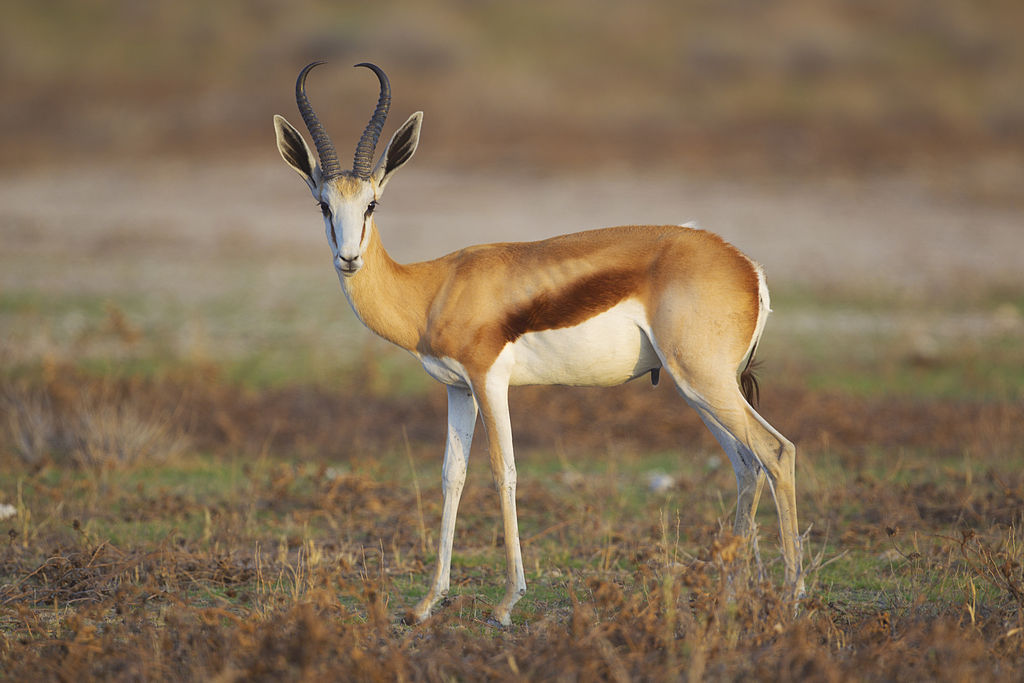
\includegraphics[width=\maxwidth{\textwidth}]{src/sample/antidorcas.jpg}
\caption{Antidorcas marsupialis, male}
\label{figure\arabic{figurecounter}}
\legend{\emph{Source}: \iftoggle{usebiblatex}{\textcite{krishnappa_adult_2012}}{\citet{krishnappa_adult_2012}}}% See: https://upload.wikimedia.org/wikipedia/commons/8/89/Antidorcas_marsupialis%2C_male_%28Etosha%2C_2012%29.jpg
\legend{\emph{Note}: Here is a note that is especially long to show what happens when it extends to more than one line.}
\end{figure}
\refstepcounter{figurecounter}
\clearpage
\section{Math examples}

This section contains some math-heavy text adapted from \iftoggle{usebiblatex}{\textcite{dwilkins1995}}{\citet{dwilkins1995}}.
In non-relativistic wave mechanics, the wave function $\psi(\mathbf{r},t)$ of a particle satisfies the Schrödinger Wave Equation
%
\begin{equation}
 i\hbar\frac{\partial \psi}{\partial t}
  = \frac{-\hbar^2}{2m} \left(
    \frac{\partial^2}{\partial x^2}
    + \frac{\partial^2}{\partial y^2}
    + \frac{\partial^2}{\partial z^2}
  \right) \psi + V \psi.
\end{equation}
%
It is customary to normalize the wave equation by
demanding that
%
\begin{equation}
\int \!\!\! \int \!\!\! \int_{\textbf{R}^3}
      \left| \psi(\mathbf{r},0) \right|^2\,dx\,dy\,dz = 1.
\end{equation}
%
A simple calculation using the Schr\"{o}dinger wave
equation shows that
%
\begin{equation}
\frac{d}{dt} \int \!\!\! \int \!\!\! \int_{\textbf{R}^3}
      \left| \psi(\mathbf{r},t) \right|^2\,dx\,dy\,dz = 0,
\end{equation}
%
and hence
%
\begin{equation}
\int \!\!\! \int \!\!\! \int_{\textbf{R}^3}
      \left| \psi(\mathbf{r},t) \right|^2\,dx\,dy\,dz = 1
\end{equation}
%
for all times~$t$. If we normalize the wave function in this
way then, for any (measurable) subset~$V$ of $\textbf{R}^3$
and time~$t$,
%
\begin{equation}
\int \!\!\! \int \!\!\! \int_V
      \left| \psi(\mathbf{r},t) \right|^2\,dx\,dy\,dz
\end{equation}
%
represents the probability that the particle is to be found
within the region~$V$ at time~$t$.

\begin{table}[h] % Table float
\caption{This caption has math characters that remain lowercase: \relax\macrocapwrap{$\psi(\mathbf{r},t)$} }
\label{table\arabic{tablecounter}}
\begin{tabu}{l c c} \\ \hline
Column1 & Column2 & Column3 \\ \hline
Row1 & 2.0 & 3.0 \\
Row2 & 2.0 & 3.0 \\
Row3 & 7.0 & 8.0 \\ \hline
\end{tabu}
\end{table}
\refstepcounter{tablecounter}
%
}{}
%%%%%%%%%%%%%%%%%%%%%%%%%%%%%%%%%%%%%%%
% Back matter
%%%%%%%%%%%%%%%%%%%%%%%%%%%%%%%%%%%%%%%
\SingleSpacing                          % Back matter should be single spaced
\AfterEndEnvironment{table}{\SingleSpacing} % Reset these environments
\AfterEndEnvironment{figure}{\SingleSpacing}
\AfterEndEnvironment{quote}{\SingleSpacing}
\AfterEndEnvironment{quotation}{\SingleSpacing}

\edef\defaulttolerance{\the\tolerance}
\tolerance 500                          % Increase tolerance to prevent material extending into margins
\hbadness 500

\iftoggle{useendnotes}{%                % If you're using endnotes, output them here
  \setsecnumdepth{none}                 % No section numbering in end notes
  \bookmarksetup{startatroot}           % Make Notes appear at root level of PDF bookmarks
  \phantomsection%                      % Need for hyperref
  \addcontentsline{toc}{chapter}{%      % Add a chapter-level heading for
    \hspace{-\cftchapterindent}%        %  Notes to the ToC
    \notesname%
  }%
  \renewcommand*{\notedivision}{%
    \chapter*{\notesname}%
  }
  \printpagenotes                       % Output the notes
  \setsecnumdepth{all}%                 % Turn section numbering back on after printing
}{}

\bookmarksetup{startatroot}
\chapter*{\bibheading}                  % In the running text, use a chapter-level heading
                                        % for the bibliography section
\phantomsection
\addcontentsline{toc}{chapter}{%        % In the TOC, add a custom chapter-level heading
  \hspace{-\cftchapterindent}%          % that will be flush against the left margin
  \bibheading%
}
%\phantomsection
%\addtocontents{toc}%                    % Add this 'mark' to TOC so subsequent pages use
%  {\protect\markboth{\bibheading}{Page}}%   the bibliography heading (unlikely since
%                                        %   the appendices follow quickly)
\iftoggle{usebiblatex}{%                % Output the bibliography
  \printbibliography[heading=none]      % Using a 'biblatex' package; do not let
                                        %   'biblatex' output a heading
}{%
  \renewcommand\bibsection{}            % Do not let 'natbib' output a heading
  \bibliographystyle{\natbibstyle}      % Using 'natbib' to print bibliography
  \bibliography{\bibfilename}
}

\appendix                               % Indicate start of appendices
                                        % Appendices are considered 'mainmatter' in this
                                        %   documentclass
\tolerance \defaulttolerance            % Set tolerance back to default
\hbadness \defaulttolerance

\addtocontents{toc}{\protect%           % Only include appendix title in table of contents
  \setcounter{tocdepth}{0}}%            %   and omit sub-headings
\renewcommand*{\chapnamefont}%          % Reset font for 'Appendix' in chapter titles
    {\normalfont\MakeTextUppercase}
\makeatletter                           % Clear page after printing appendix title
  \renewcommand{\memendofchapterhook}%
  {%
    \clearpage
    \m@mindentafterchapter
    \@afterheading
  }
\makeatother

\phantomsection                         % Need '\phantomsection' to place hyperref
                                        %   bookmark more accurately
\addcontentsline{toc}{part}{Appendix}   %~Add "Appendix" to TOC here; comment out this
                                        %   line if you're not including appendices

%\phantomsection                        %!This is the one part of the template that I
%\addtocontents{toc}%                   %   could not get to work properly. After you
%  {\protect\markboth{APPENDIX}{Page}}  %   start listing appendices in the TOC,
                                        %   subsequent TOC pages should use "APPENDIX in
                                        %   the header instead of "CHAPTER"; however,
                                        %   this code will make "APPENDIX" appear on the
                                        %   the same page that the *first* appendix
                                        %   appears on. This problem won't affect most
                                        %   people, but if it affects you, uncomment
                                        %   these lines and move them below where
                                        %   the appendices are listed. Keep moving these
                                        %   lines down and checking the output until
                                        %   the TOC headers appear correctly

\chapter{This is a chapter-level heading for an appendix}

\lipsum[1]

\section{This is the first section-level heading in the appendix}

\lipsum[1]

\subsection{This is the first sub-section-level heading in the appendix}

\lipsum[1]

\subsubsection{This is the first sub-sub-section-level heading in the appendix}

\lipsum[1]

\paragraph{This is the first paragraph-level heading in the appendix}

\lipsum[1]

\subparagraph{This is the first sub-paragraph-level heading in the appendix}

\lipsum[1]                        %~Insert your appendices here; I recommend to use
%\input{appendix2}                       %   \input rather than \include for appendices.
%\input{appendix3}% etc.                 %   All heading commands are the same as above,
                                         %   e.g., \chapter, \section, etc.
\iftoggle{sample}{%
  \chapter{This is a chapter-level heading for an appendix}

\lipsum[1]

\section{This is the first section-level heading in the appendix}

\lipsum[1]

\subsection{This is the first sub-section-level heading in the appendix}

\lipsum[1]

\subsubsection{This is the first sub-sub-section-level heading in the appendix}

\lipsum[1]

\paragraph{This is the first paragraph-level heading in the appendix}

\lipsum[1]

\subparagraph{This is the first sub-paragraph-level heading in the appendix}

\lipsum[1] %
}{}

\backmatter                             % Start back matter according to documentclass
\makeatletter                           % Do not clear page after printing title for
  \renewcommand{\memendofchapterhook}%  %   biographical sketch
  {%
    \m@mindentafterchapter
    \@afterheading
  }
\makeatother

%\biographicalsketch{%                  %~Biographical Sketch is optional
%  \input{biography}%                   %<Enter the name of the .tex file containing your
%}%                                     %   biography or omit this line and type in
                                        %   your biography here (1 paragraph)
\end{document}
